%!TeX root = main.tex
%!encoding = UTF-8 Unicode


\section{Verification}

This section verifies the active current shunt in both the frequency and time domain.
Because the shunt is intended to resolve high-frequency commutation currents while preserving the low-frequency switching waveform, the verification must demonstrate not only the expected transfer behavior of the two filter paths, but also the overall usability of the probe in a measurement setup with finite source impedance and strong common-mode disturbance.

Accordingly, the verification is divided into a small-signal characterization using a vector network analyzer (VNA) and a large-signal validation using a passive shunt reference measurement.
The small-signal tests confirm the transfer functions of the low-pass and high-pass channels, while the large-signal tests assess the probe response under realistic switching conditions and verify that the active shunt does not introduce relevant distortion into the measured waveform.

\subsection{Small-Signal}

The VNA measurements of the low-pass and high-pass channels are shown in \fref{fig:VNA_Shunt_LP} and \fref{fig:VNA_Shunt_HP}.
For the low-pass path, the measured transfer includes the complete signal chain from the passive shunt through the compensation amplifier and low-pass filter to the VNA input.
The low-pass channel exhibits a bandwidth of \mi{f}{3dB} = \SI{475}{MHz} before the gain begins to rise.
Compared with the compensation-amplifier transfer function in \fref{fig:VNA_CompAmp}, this gain increase occurs at a higher frequency.
The reason is that the higher gain delays the point at which the secondary parasitic transmission path becomes dominant.
This bandwidth is more than sufficient for the intended SiC discrete-device measurements, where the noise floor typically starts to rise around \SI{100}{MHz}.
	
\begin{figure}[ht]
	\centering
	% This file was created by matlab2tikz.
%
%The latest updates can be retrieved from
%  http://www.mathworks.com/matlabcentral/fileexchange/22022-matlab2tikz-matlab2tikz
%where you can also make suggestions and rate matlab2tikz.
%
\definecolor{mycolor1}{rgb}{0.00000,0.44700,0.74100}%
\definecolor{mycolor2}{rgb}{0.85000,0.32500,0.09800}%
\definecolor{mycolor3}{rgb}{0.92900,0.69400,0.12500}%
\definecolor{mycolor4}{rgb}{0.49400,0.18400,0.55600}%
%
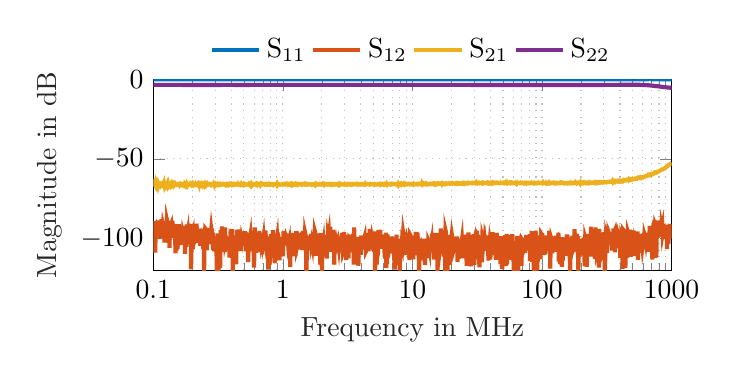
\begin{tikzpicture}

\begin{axis}[%
width=2.591in,
height=0.957in,
at={(0.616in,0.474in)},
scale only axis,
unbounded coords=jump,
xmode=log,
xmin=0.1,
xmax=1000,
xtick={0.1,1,10,100,1000},
xticklabels={{0.1},{1},{10},{100},{1000}},
xminorticks=true,
xlabel style={font=\color{white!15!black}},
xlabel={Frequency in MHz},
ymin=-120,
ymax=0,
ylabel style={font=\color{white!15!black}},
ylabel={Magnitude in dB},
axis background/.style={fill=white},
xmajorgrids,
xminorgrids,
ymajorgrids,
grid style={dotted},
legend style={at={(0.5,1.03)}, anchor=south, legend cell align=left, align=left, fill=none, draw=none},
legend columns = 4
]
\addplot [color=mycolor1, line width=1.5pt]
  table[row sep=crcr]{%
0.1	-0.01816616493\\
0.106349442	-0.01690826572\\
0.112698884	-0.01177073301\\
0.138482796	-0.009570624616\\
0.1725446	-0.01002667798\\
0.198281036	-0.01491078476\\
0.219753858	-0.01122766743\\
0.291109957	-0.01453728435\\
0.344627992	-0.0144176859\\
0.446255517	-0.01466776159\\
0.497605565	-0.01379297952\\
0.546753616	-0.01510196244\\
1.632240533	-0.01508187313\\
11.99531021	-0.02139159331\\
18.85543879	-0.02558769899\\
32.03721498	-0.03286254809\\
39.73397101	-0.03657987226\\
53.70000506	-0.04281928757\\
131.4730623	-0.06950909163\\
282.7730138	-0.1017708403\\
329.0158078	-0.1111759172\\
344.0396394	-0.09936534832\\
350.4784243	-0.1029096142\\
359.0634709	-0.09087256654\\
371.9410408	-0.1019650848\\
380.5260874	-0.09073750277\\
401.988704	-0.1054924715\\
417.0125355	-0.1042022018\\
428.4054685	-0.1084264984\\
431.3651992	-0.1033617309\\
434.32493	-0.1100306159\\
440.2443915	-0.101593645\\
446.163853	-0.1114931586\\
458.0027759	-0.112084918\\
469.8416989	-0.1111202812\\
481.6806219	-0.1132454342\\
487.6000834	-0.1234797659\\
499.4390064	-0.1098537975\\
502.3987372	0.07314965416\\
nan	nan\\
511.2779294	0.007344708969\\
514.2376601	-0.1122263874\\
517.1973909	-0.08214171247\\
520.1571216	0.1105124474\\
nan	nan\\
529.0363139	0.02889304633\\
537.9155061	-0.1208650818\\
573.4322751	-0.1137035457\\
576.8889099	0.2672458068\\
nan	nan\\
589.0986518	0.03818298189\\
601.3083936	-0.1211315156\\
613.5181355	-0.1290170649\\
646.0774471	-0.1243407895\\
654.217275	-0.1171832491\\
658.2871889	0.3247927109\\
nan	nan\\
690.8465005	0.2813638476\\
703.0562424	-0.129694273\\
711.1960703	-0.06261471623\\
715.2659843	-0.1322730956\\
739.685468	-0.1510730607\\
764.1049517	-0.1448210481\\
788.5244354	-0.149208805\\
826.9631436	-0.1606742902\\
894.3341504	-0.1472239124\\
944.8624056	-0.1612820546\\
989.7764101	-0.1487663639\\
1001.004911	-0.1477712303\\
};
\addlegendentry{$\mathrm{S}_\mathrm{11}$}

\addplot [color=mycolor2, line width=1.5pt]
  table[row sep=crcr]{%
0.1	-90.56814014\\
0.100705494	-96.88295613\\
0.101410987	-89.07895684\\
0.102116481	-92.1975316\\
0.102821974	-91.81817866\\
0.103527468	-108.7492756\\
0.104232961	-93.74855862\\
0.104938455	-96.52511842\\
0.105643948	-96.30135231\\
0.107054935	-90.43724334\\
0.107760429	-95.91269435\\
0.108465922	-90.67295735\\
0.109876909	-100.0705598\\
0.110582403	-88.55027834\\
0.112698884	-96.1189421\\
0.113404377	-91.74383941\\
0.114109871	-99.49870695\\
0.115520858	-87.79120717\\
0.116226351	-90.50936768\\
0.116931845	-88.3328983\\
0.117637338	-98.36369265\\
0.119048325	-91.31574339\\
0.119753819	-92.17853912\\
0.120459312	-88.92292899\\
0.121164806	-91.81123625\\
0.1218703	-102.4405326\\
0.12398678	-89.55752108\\
0.124692274	-94.36806555\\
0.125397767	-93.0604946\\
0.126103261	-99.03173997\\
0.126808754	-96.94754445\\
0.127514248	-88.28775528\\
0.128925235	-90.01807606\\
0.129630728	-101.799078\\
0.131041715	-91.73995317\\
0.131747209	-102.6379645\\
0.132452703	-88.92096064\\
0.133158196	-105.7292538\\
0.134569183	-93.69902266\\
0.135274677	-96.43961683\\
0.13598017	-89.03906886\\
0.136685664	-91.32038958\\
0.137509601	-90.75663574\\
0.13945599	-97.29351284\\
0.140429185	-88.68162591\\
0.141402379	-98.50200252\\
0.142375573	-94.49769312\\
0.144321962	-99.40118738\\
0.146268351	-90.89506769\\
0.147241545	-93.52950038\\
0.14821474	-109.2142064\\
0.149187934	-99.44652422\\
0.151134323	-107.4688956\\
0.152107517	-91.10842569\\
0.153080712	-93.76825211\\
0.154053906	-106.5895076\\
0.155027101	-94.25361451\\
0.156000295	-97.44637535\\
0.156973489	-90.91016526\\
0.157946684	-102.1954493\\
0.159893073	-96.96360246\\
0.160866267	-103.9437463\\
0.162812656	-94.91851954\\
0.164759045	-97.64917746\\
0.165732239	-103.6003035\\
0.168651822	-96.19457427\\
0.170598211	-98.04391858\\
0.171571405	-94.04637387\\
0.1725446	-100.9946312\\
0.174490989	-94.87234767\\
0.175464183	-109.5653393\\
0.176437377	-92.17250439\\
0.177410572	-101.8272965\\
0.178383766	-93.17557544\\
0.179356961	-105.128516\\
0.181303349	-91.08722571\\
0.183249738	-97.19080822\\
0.184222933	-96.07220291\\
0.186169321	-103.5422885\\
0.187142516	-97.72503852\\
0.18811571	-101.7483645\\
0.189088905	-90.62783753\\
0.190228728	-98.11155619\\
0.194254882	-90.87532806\\
0.195596933	-119.2363945\\
0.198281036	-98.11458012\\
0.199623087	-98.28011993\\
0.200965139	-97.27804111\\
0.20230719	-106.7054686\\
0.204991293	-97.3539136\\
0.206333344	-99.56957007\\
0.207675395	-92.38492743\\
0.213043601	-100.9380642\\
0.214385652	-100.6018674\\
0.215727704	-90.53388552\\
0.217069755	-96.61927159\\
0.218411806	-94.3173419\\
0.22243796	-102.5012777\\
0.225122063	-95.41696508\\
0.226464115	-102.7431429\\
0.227806166	-94.73613904\\
0.230490269	-104.4733699\\
0.23183232	-93.67556649\\
0.235858474	-102.4307894\\
0.238542577	-96.00652682\\
0.239884628	-103.9823073\\
0.24122668	-97.75074053\\
0.242568731	-106.4061834\\
0.245252834	-94.53319844\\
0.246594885	-125.9872536\\
0.247936937	-95.11894462\\
0.249278988	-107.1224183\\
0.251963091	-93.58772367\\
0.253305142	-93.83153168\\
0.254647193	-95.45837927\\
0.258673347	-107.3126867\\
0.260015399	-97.76960141\\
0.261582765	-101.8154612\\
0.263428214	-93.45047028\\
0.267119113	-103.5028065\\
0.270810012	-95.43297372\\
0.272655462	-102.887244\\
0.274500911	-96.35553487\\
0.276346361	-98.80387366\\
0.28003726	-93.99952971\\
0.281882709	-95.88844321\\
0.283728159	-93.59180995\\
0.285573608	-100.4580955\\
0.287419058	-96.17143861\\
0.289264507	-107.0144256\\
0.292955406	-101.0675425\\
0.294800856	-107.9337457\\
0.296646305	-100.1066814\\
0.298491755	-101.641747\\
0.300337204	-98.74623031\\
0.302182654	-104.8543312\\
0.304028103	-99.05339456\\
0.307719002	-109.7219324\\
0.309564452	-121.7804001\\
0.313255351	-96.67479573\\
0.3151008	-102.7394325\\
0.31694625	-130.1769687\\
0.320637149	-97.64177041\\
0.328018947	-118.5072505\\
0.331709845	-94.6478901\\
0.333555295	-106.0616617\\
0.339091643	-92.40581835\\
0.342782542	-104.967175\\
0.35016434	-96.94048684\\
0.355700689	-108.3856725\\
0.357546138	-92.98296302\\
0.359701417	-100.0942542\\
0.362247126	-98.7064259\\
0.364792835	-99.48620559\\
0.367338544	-106.2055218\\
0.369884252	-99.3023719\\
0.372429961	-101.7783577\\
0.37497567	-99.17569079\\
0.377521379	-104.2411042\\
0.380067088	-99.87871133\\
0.385158505	-104.296773\\
0.387704214	-111.9151803\\
0.392795632	-100.4552064\\
0.395341341	-101.1546618\\
0.402978467	-94.02670996\\
0.405524176	-104.6603056\\
0.408069885	-103.3247741\\
0.410615594	-121.3016594\\
0.413161302	-103.8561422\\
0.415707011	-109.4272418\\
0.41825272	-98.57397695\\
0.423344138	-106.0133229\\
0.428435555	-99.89984324\\
0.430981264	-103.3912689\\
0.433526973	-98.01088196\\
0.436072682	-116.1236918\\
0.441164099	-94.3200908\\
0.443709808	-99.29965529\\
0.446255517	-96.78110731\\
0.451346935	-105.5900237\\
0.453892644	-103.9076726\\
0.458984061	-94.22124142\\
0.466621188	-107.7582742\\
0.471712605	-99.86733052\\
0.474258314	-102.9409465\\
0.479349732	-99.31917373\\
0.484441149	-100.9278441\\
0.486986858	-98.94312937\\
0.489532567	-99.14041244\\
0.492078276	-98.72005423\\
0.494623985	-95.99858932\\
0.497605565	-104.4427675\\
0.50111614	-99.44640328\\
0.504626715	-103.0030652\\
0.50813729	-95.27773646\\
0.511647866	-104.4690589\\
0.515158441	-95.85374201\\
0.522179591	-107.9350318\\
0.525690166	-97.60990704\\
0.529200741	-102.8353866\\
0.532711316	-96.23928503\\
0.539732466	-114.6393015\\
0.546753616	-98.56870904\\
0.550264191	-102.4631852\\
0.560795917	-98.37952697\\
0.567817067	-107.8490521\\
0.574838217	-103.0100341\\
0.581859367	-106.8714284\\
0.585369942	-95.37261074\\
0.588880517	-97.66101408\\
0.592391092	-97.31925449\\
0.599412243	-118.1356477\\
0.606433393	-92.95429957\\
0.616965118	-108.9167858\\
0.620475693	-98.22781809\\
0.623986268	-104.8861125\\
0.627496843	-102.850243\\
0.631007418	-96.06846619\\
0.634517993	-101.6985767\\
0.638028568	-101.2768765\\
0.641539144	-96.46365963\\
0.652070869	-108.5159635\\
0.659092019	-95.17700201\\
0.662602594	-107.0348496\\
0.673134319	-97.00897964\\
0.680155469	-101.5161732\\
0.684255429	-100.0817493\\
0.693940768	-109.7600515\\
0.698783437	-96.90484079\\
0.703626107	-101.0172012\\
0.708468776	-99.37002939\\
0.713311446	-102.9295627\\
0.718154115	-101.0065509\\
0.722996785	-107.5726127\\
0.732682124	-94.84210524\\
0.742367463	-100.6176711\\
0.747210132	-98.71763792\\
0.756895471	-106.662915\\
0.76658081	-100.7898886\\
0.77142348	-119.410664\\
0.776266149	-102.0277923\\
0.781108819	-107.105402\\
0.785951488	-99.72058834\\
0.790794158	-116.6009072\\
0.795636827	-99.35835234\\
0.805322166	-110.6359316\\
0.810164836	-97.10149137\\
0.815007505	-101.5595078\\
0.824692844	-99.13791508\\
0.829535514	-111.9498816\\
0.839220853	-94.67555332\\
0.844063522	-100.5435047\\
0.848906192	-100.5015727\\
0.853748861	-104.9827186\\
0.858591531	-102.1070009\\
0.8634342	-115.2590776\\
0.877962209	-99.7546645\\
0.882804878	-103.7571193\\
0.902175556	-99.03516778\\
0.907018226	-103.0042834\\
0.911860895	-96.06807582\\
0.916703565	-105.2348117\\
0.921546234	-97.3711783\\
0.926388904	-104.7945842\\
0.931231573	-104.0443067\\
0.936074243	-99.04006054\\
0.940916912	-113.5838051\\
0.953266857	-99.96938314\\
0.973301224	-107.9651885\\
0.979979347	-98.90421329\\
1.000013714	-111.0078168\\
1.013369958	-95.24530653\\
1.02004808	-102.1843343\\
1.026726203	-95.46046445\\
1.033404325	-101.3400746\\
1.040082447	-97.34320806\\
1.04676057	-102.1668012\\
1.060116814	-99.00266486\\
1.066794937	-99.70182082\\
1.073473059	-103.6518439\\
1.080151181	-96.67064195\\
1.086829304	-104.2649786\\
1.093507426	-101.2920884\\
1.100185548	-104.3573016\\
1.120219915	-101.3997585\\
1.126898037	-105.4682464\\
1.13357616	-96.80893129\\
1.140254282	-117.7892034\\
1.146932404	-96.75616418\\
1.153610527	-104.9796716\\
1.160288649	-99.03046897\\
1.173644894	-111.0239729\\
1.180323016	-100.834764\\
1.187001138	-104.0158785\\
1.19367926	-102.5107078\\
1.200357383	-96.37118614\\
1.213713627	-101.9271092\\
1.22039175	-98.19952102\\
1.227069872	-107.0444695\\
1.233747994	-100.261753\\
1.253782361	-111.1088514\\
1.267138606	-95.28673389\\
1.273816728	-96.7944818\\
1.28049485	-95.66706904\\
1.287172973	-105.3399827\\
1.293851095	-104.581597\\
1.301650396	-97.89288158\\
1.310833455	-106.1220519\\
1.320016515	-98.87270661\\
1.338382633	-104.7792776\\
1.347565693	-100.0308235\\
1.356748752	-102.3455292\\
1.365931811	-98.01152873\\
1.375114871	-98.12120797\\
1.38429793	-99.63047565\\
1.393480989	-107.0879598\\
1.411847108	-96.07594913\\
1.421030167	-98.11301999\\
1.430213227	-95.12464247\\
1.448579346	-103.8809408\\
1.457762405	-100.9596231\\
1.466945464	-101.3239998\\
1.476128524	-104.2875282\\
1.485311583	-96.40166838\\
1.494494642	-97.4146711\\
1.512860761	-109.7909069\\
1.52204382	-129.988048\\
1.53122688	-98.99125741\\
1.549592999	-106.5986054\\
1.558776058	-98.09860042\\
1.567959117	-102.6698187\\
1.577142177	-101.6461807\\
1.586325236	-101.8775435\\
1.595508295	-107.4096705\\
1.613874414	-99.58112694\\
1.641423592	-105.9951884\\
1.650606652	-97.04304203\\
1.659789711	-102.0718586\\
1.66897277	-101.0371944\\
1.687338889	-103.5170687\\
1.696521948	-100.1605037\\
1.705705008	-103.1609537\\
1.714888067	-96.47240996\\
1.733254186	-110.9287005\\
1.751620305	-98.23429005\\
1.760803364	-108.6507617\\
1.769986423	-95.47511692\\
1.779169483	-96.14068671\\
1.78989427	-102.0280033\\
1.802561859	-96.82376844\\
1.815229447	-106.3928257\\
1.827897036	-103.8091524\\
1.840564625	-103.8750251\\
1.865899803	-110.6437926\\
1.878567391	-97.86157248\\
1.916570158	-102.6862545\\
1.929237746	-100.8086192\\
1.941905335	-116.1838968\\
1.954572924	-96.45921063\\
2.005243279	-120.3605316\\
2.017910868	-100.5966846\\
2.030578457	-105.0429688\\
2.055913634	-102.1834404\\
2.081248812	-109.234148\\
2.0939164	-98.48557316\\
2.144586756	-103.280029\\
2.169921933	-99.41589143\\
2.182589522	-112.543903\\
2.207924699	-97.68361921\\
2.220592288	-108.02314\\
2.233259877	-98.16026105\\
2.245927466	-99.09950795\\
2.271262643	-96.43093057\\
2.30926541	-106.0274676\\
2.321932998	-92.52325491\\
2.334600587	-103.9445953\\
2.347268176	-99.23588569\\
2.359935765	-108.2546251\\
2.372603353	-97.61838567\\
2.397938531	-106.2536618\\
2.423273708	-100.7978159\\
2.435941297	-102.4964457\\
2.461276475	-94.48744063\\
2.476112985	-97.23917909\\
2.493581802	-116.1855415\\
2.511050619	-97.9981374\\
2.545988253	-106.4041754\\
2.598394704	-102.5259646\\
2.615863521	-104.2300445\\
2.633332338	-97.44267949\\
2.668269972	-108.5900921\\
2.685738789	-104.1118537\\
2.703207606	-105.826885\\
2.720676423	-103.4786719\\
2.73814524	-104.5963689\\
2.755614057	-104.3526892\\
2.790551691	-99.04251809\\
2.825489325	-106.9919229\\
2.860426959	-102.845944\\
2.877895776	-96.35135316\\
2.91283341	-108.5570425\\
2.930302227	-107.9271813\\
2.965239861	-95.86047381\\
3.017646312	-104.7479304\\
3.035115129	-98.17483899\\
3.087521579	-113.4208627\\
3.122459213	-103.3506184\\
3.13992803	-107.93347\\
3.157396847	-97.83066932\\
3.174865664	-110.5656193\\
3.192334481	-108.4109307\\
3.209803298	-112.3637158\\
3.227272115	-103.6661485\\
3.244740932	-106.8191796\\
3.262209749	-99.21771398\\
3.279678566	-99.40733086\\
3.297147383	-105.6905533\\
3.3146162	-97.55476746\\
3.332085017	-102.8352344\\
3.349553834	-100.0255232\\
3.367022651	-105.2374507\\
3.384491468	-105.0447384\\
3.404893095	-100.4521677\\
3.428914395	-108.408841\\
3.476956996	-97.10126839\\
3.500978297	-100.1245677\\
3.524999597	-116.2252111\\
3.549020898	-92.97552383\\
3.597063499	-114.4102031\\
3.6210848	-104.001956\\
3.6451061	-104.3720709\\
3.669127401	-98.96379137\\
3.693148702	-103.6858664\\
3.717170002	-98.97514439\\
3.741191303	-101.2375431\\
3.765212603	-113.3585423\\
3.789233904	-102.944717\\
3.813255204	-116.9128489\\
3.837276505	-114.4895321\\
3.861297806	-102.2637635\\
3.885319106	-109.8836921\\
3.909340407	-100.7184014\\
3.933361707	-103.5154335\\
3.957383008	-99.29868857\\
3.981404309	-110.0047071\\
4.005425609	-108.7532157\\
4.02944691	-97.99820435\\
4.05346821	-102.9173045\\
4.077489511	-102.7858575\\
4.101510811	-100.6932613\\
4.125532112	-104.4271594\\
4.173574713	-99.22592949\\
4.197596014	-101.3655614\\
4.269659915	-99.13022669\\
4.293681216	-104.5964514\\
4.365745118	-97.19761462\\
4.389766418	-107.7470692\\
4.413787719	-107.3441486\\
4.43780902	-100.6927011\\
4.485851621	-107.8051678\\
4.509872921	-96.42095416\\
4.533894222	-104.9092002\\
4.557915522	-102.1928865\\
4.581936823	-107.8077933\\
4.629979424	-103.3199803\\
4.654000725	-105.7591983\\
4.68205492	-93.84584795\\
4.748327378	-103.3663417\\
4.781463607	-98.07907732\\
4.814599836	-102.9918901\\
4.847736065	-100.4630988\\
4.880872294	-103.7754171\\
4.914008523	-99.72001304\\
4.947144752	-100.7502665\\
4.980280981	-107.4135139\\
5.01341721	-100.8972592\\
5.046553439	-108.254108\\
5.112825896	-95.40622584\\
5.145962125	-121.4938877\\
5.212234583	-101.2575159\\
5.245370812	-102.7331586\\
5.278507041	-98.44446745\\
5.31164327	-116.2424764\\
5.377915728	-107.1312177\\
5.411051957	-110.4873193\\
5.477324415	-94.46056424\\
5.543596873	-102.2200751\\
5.576733102	-95.46642933\\
5.609869331	-101.989194\\
5.64300556	-94.53572817\\
5.676141789	-105.9321463\\
5.742414247	-99.13031851\\
5.841822933	-106.2777\\
5.974367849	-97.3462899\\
6.007504078	-105.2532015\\
6.040640307	-102.9905792\\
6.073776536	-103.3600028\\
6.106912765	-111.3268007\\
6.140048994	-99.95611857\\
6.173185223	-112.4366744\\
6.239457681	-96.1673531\\
6.27259391	-118.3769683\\
6.338866368	-99.31099205\\
6.372002597	-116.1203822\\
6.438275055	-97.31541267\\
6.477084809	-111.8483265\\
6.614171052	-103.0425699\\
6.659866467	-109.3247705\\
6.751257296	-102.0557652\\
6.842648125	-108.4950819\\
6.934038953	-98.63616271\\
7.025429782	-103.7056372\\
7.071125197	-100.2534472\\
7.116820611	-105.3857897\\
7.162516026	-102.2349102\\
7.299602269	-119.4288202\\
7.345297683	-105.1064121\\
7.436688512	-116.5781767\\
7.482383927	-113.6842071\\
7.528079341	-97.55592385\\
7.573774756	-104.5532669\\
7.61947017	-104.5068858\\
7.665165585	-105.9748054\\
7.710860999	-103.2704047\\
7.756556413	-106.6973808\\
7.802251828	-106.1996295\\
7.847947242	-101.5514406\\
7.893642657	-107.6135208\\
7.939338071	-105.7676101\\
7.985033486	-119.936883\\
8.076424314	-100.2060775\\
8.122119729	-104.5983132\\
8.167815143	-102.2158551\\
8.259205972	-109.353251\\
8.304901387	-104.2507969\\
8.350596801	-105.1630275\\
8.487683044	-96.14441715\\
8.533378459	-97.33585096\\
8.624769288	-108.9547116\\
8.670464702	-100.4514836\\
8.716160117	-106.525955\\
8.761855531	-106.0838523\\
8.807550946	-99.26815508\\
8.85324636	-110.1133065\\
8.906613499	-101.1617967\\
8.969648125	-104.182019\\
9.095717379	-99.85854277\\
9.158752005	-100.7381466\\
9.221786632	-103.6087497\\
9.284821259	-103.0353068\\
9.347855886	-98.7752776\\
9.410890512	-101.9567698\\
9.473925139	-113.3920963\\
9.599994392	-97.57948363\\
9.663029019	-98.00529745\\
9.726063646	-104.4051768\\
9.852132899	-103.3778471\\
9.915167526	-107.3160642\\
9.978202153	-98.15785171\\
10.16730603	-112.9029334\\
10.23034066	-100.5009127\\
10.29337529	-104.5711793\\
10.35640991	-104.1774224\\
10.41944454	-99.66630027\\
10.54551379	-110.489602\\
10.60854842	-95.7810518\\
10.67158305	-104.6778239\\
10.73461767	-96.77145269\\
10.86068693	-99.736514\\
10.92372155	-96.21557573\\
11.11282543	-105.074408\\
11.17586006	-100.4196802\\
11.23889469	-125.2216212\\
11.36496394	-103.0524117\\
11.42799857	-103.5427282\\
11.49103319	-103.1695215\\
11.61710245	-106.7073558\\
11.68013707	-111.1018577\\
11.80620633	-102.0395549\\
11.93227558	-106.0911415\\
12.05834483	-100.0303471\\
12.18441409	-113.5098908\\
12.24744871	-100.3148016\\
12.49512763	-116.4808008\\
12.66897924	-101.1137114\\
12.84283085	-111.6149175\\
13.10360827	-99.86924587\\
13.19053407	-112.0975335\\
13.27745988	-100.9085908\\
13.36438568	-101.4359221\\
13.6251631	-106.2209525\\
13.7120889	-103.1009196\\
13.79901471	-105.4447674\\
14.05979212	-101.6185695\\
14.14671793	-106.2544132\\
14.23364374	-96.82177346\\
14.40749535	-104.8320763\\
14.49442115	-98.65915608\\
14.58134696	-102.4944188\\
14.66827276	-96.33870635\\
14.75519857	-113.1100077\\
14.84212437	-97.94839819\\
14.92905018	-108.8364294\\
15.10290179	-98.27899059\\
15.1898276	-104.7074143\\
15.36367921	-103.7118686\\
15.45060501	-96.38770883\\
15.53753082	-101.7002791\\
15.62445662	-121.0336886\\
15.88523404	-101.8332245\\
15.97215985	-103.4543562\\
16.05908565	-111.7238246\\
16.14601146	-101.4823636\\
16.31986307	-106.9503541\\
16.40678887	-105.5667195\\
16.58064048	-93.5258053\\
16.75449209	-108.0177462\\
16.8414179	-101.0582462\\
17.06246886	-107.2901129\\
17.18200019	-100.7121799\\
17.30153151	-109.4370703\\
17.42106284	-104.0052187\\
17.54059417	-111.137184\\
17.77965683	-97.13903254\\
17.89918816	-120.9399907\\
18.01871949	-94.79752829\\
18.13825081	-95.81209807\\
18.25778214	-104.3442636\\
18.37731347	-99.79912512\\
18.61637613	-120.699647\\
18.85543878	-98.36422122\\
18.97497011	-108.4987018\\
19.09450144	-107.293994\\
19.21403277	-112.1300778\\
19.3335641	-97.6670215\\
19.45309543	-116.3903024\\
19.81168941	-98.79942783\\
19.93122074	-100.2584571\\
20.05075207	-100.0089234\\
20.1702834	-97.60676933\\
20.40934606	-100.1599165\\
20.52887738	-104.5147586\\
20.64840871	-99.05243801\\
20.76794004	-100.5289032\\
20.88747137	-106.8454623\\
21.0070027	-106.1913867\\
21.12653403	-100.5683275\\
21.36559668	-104.2543398\\
21.48512801	-103.9491682\\
21.60465934	-106.5157829\\
21.72419067	-100.8816329\\
21.96325333	-105.8045933\\
22.08278466	-98.64333785\\
22.32184731	-114.5968047\\
22.44137864	-100.2561866\\
22.56090997	-108.395908\\
22.6804413	-102.0047276\\
22.79997263	-112.6605871\\
23.15856661	-101.4806098\\
23.29816585	-106.9131687\\
23.46305357	-101.4656807\\
23.62794129	-105.7237143\\
24.12260445	-100.5359951\\
24.6172676	-112.3170312\\
24.78215532	-105.6762972\\
24.94704304	-109.1926634\\
25.11193076	-103.9351172\\
25.27681848	-108.6072582\\
25.77148164	-97.4862448\\
26.2661448	-117.0702488\\
26.43103252	-99.1015304\\
26.59592024	-103.9927546\\
27.09058339	-96.09252468\\
27.25547111	-100.9809284\\
27.42035883	-97.90188548\\
27.75013427	-106.4420731\\
27.91502199	-102.9540502\\
28.07990971	-105.5203767\\
28.24479743	-103.8278137\\
28.40968515	-117.3381457\\
28.73946059	-98.04087771\\
29.23412375	-115.7610587\\
29.56389918	-97.170193\\
29.7287869	-101.7120663\\
29.89367462	-101.0074288\\
30.05856234	-116.4299144\\
30.22345006	-99.38171413\\
30.5532255	-112.0385261\\
31.04788866	-103.1181861\\
31.21277638	-111.5598036\\
31.54255182	-94.91355164\\
31.87232726	-113.0707946\\
32.03721498	-98.4279178\\
32.23033447	-98.81393592\\
32.91248325	-117.9904267\\
33.3672491	-102.5712762\\
33.59463202	-112.6228468\\
34.04939788	-100.5469754\\
34.2767808	-103.5471706\\
34.50416373	-114.876164\\
34.73154665	-99.01798415\\
35.1863125	-100.8045028\\
35.41369543	-96.42482891\\
35.64107835	-100.4431081\\
35.86846128	-99.60468551\\
36.0958442	-102.7683149\\
36.32322713	-99.23169353\\
36.55061005	-100.2671229\\
36.77799298	-106.1139925\\
37.00537591	-101.9562073\\
37.23275883	-107.5501145\\
37.68752468	-98.23289361\\
37.91490761	-105.1329774\\
38.36967346	-101.0452321\\
38.59705638	-113.6813455\\
39.05182223	-97.93058213\\
39.27920516	-104.7694771\\
39.50658808	-102.3449822\\
39.73397101	-103.8087131\\
39.96135393	-113.151412\\
40.41611978	-96.41016523\\
41.32565149	-107.0714129\\
41.55303441	-95.90860683\\
41.78041734	-108.3265548\\
42.00780026	-99.52465233\\
42.68994904	-106.2166856\\
42.91733196	-97.06829364\\
43.37209781	-110.3458015\\
43.59948074	-96.72012891\\
44.05424659	-113.2840266\\
44.6324778	-96.42823365\\
44.94515115	-98.1831171\\
45.2578245	-107.866068\\
45.57049786	-103.2016945\\
45.88317121	-104.8364973\\
46.19584457	-110.9854583\\
46.50851792	-102.6210135\\
46.82119127	-105.2465961\\
47.44653798	-101.1457361\\
47.75921134	-115.7203619\\
48.07188469	-98.42635073\\
48.6972314	-104.7063795\\
49.00990475	-103.3876973\\
49.32257811	-119.0700147\\
49.94792482	-99.94388143\\
50.26059817	-107.4359901\\
50.57327152	-100.7593741\\
50.88594488	-108.83765\\
51.19861823	-108.2803946\\
51.51129158	-106.379699\\
52.13663829	-97.82343616\\
52.44931165	-117.1537882\\
52.761985	-103.1182298\\
53.07465836	-107.8529314\\
53.38733171	-97.04088072\\
53.70000506	-116.2125673\\
54.63802513	-98.58131858\\
55.57604519	-112.3497267\\
55.88871854	-100.1773018\\
56.2013919	-109.0256758\\
56.51406525	-99.13395697\\
56.82673861	-113.2162589\\
57.13941196	-97.62471135\\
57.45208531	-104.8246711\\
57.76475867	-97.6858269\\
58.07743202	-103.2748771\\
58.39010537	-100.2689931\\
58.70277873	-101.8249307\\
59.01545208	-97.23761276\\
59.32812544	-98.88580104\\
59.64079879	-107.8907618\\
59.95347215	-107.7572301\\
60.2661455	-108.9370886\\
60.57881885	-125.4892862\\
61.37530425	-103.8916138\\
62.66925782	-115.5125698\\
63.10057567	-101.9712988\\
63.53189353	-104.3029203\\
63.96321139	-111.0902419\\
64.39452924	-98.48771147\\
64.82584709	-110.7365381\\
65.25716495	-109.5446954\\
65.68848281	-120.7459559\\
66.11980066	-99.36713621\\
66.55111852	-114.2536443\\
67.41375423	-99.03663301\\
68.27638994	-107.8803463\\
69.13902565	-99.827425\\
69.5703435	-117.0685884\\
70.00166136	-100.4531427\\
70.43297921	-100.7972343\\
70.86429707	-110.0437879\\
71.29561493	-99.48004579\\
72.15825064	-107.9988958\\
73.02088635	-104.226548\\
73.88352206	-108.9135868\\
74.31483991	-107.0828876\\
74.74615777	-99.75726961\\
75.17747562	-105.1868803\\
75.60879348	-97.66538559\\
76.47142919	-107.2045872\\
77.76538276	-99.78460541\\
78.19670061	-102.5264494\\
79.05933632	-97.8071234\\
79.49065418	-105.8476678\\
80.35328989	-97.40448818\\
80.78460774	-114.0981803\\
81.2159256	-97.21674313\\
81.64724345	-107.2928717\\
82.07856131	-107.1709299\\
83.37251487	-95.23015213\\
83.80383273	-114.6715825\\
84.30900005	-104.9330234\\
84.90379459	-107.561065\\
85.49858914	-101.7788235\\
86.68817822	-123.2716988\\
87.28297277	-102.4064066\\
87.87776731	-130.2849667\\
89.0673564	-95.2039152\\
89.66215094	-96.89446858\\
90.85174002	-115.9332063\\
91.44653457	-98.01852545\\
92.04132911	-120.0881441\\
92.63612365	-99.7725944\\
93.82571274	-108.3502423\\
95.01530183	-102.2537023\\
95.61009637	-106.986598\\
96.79968545	-104.1947785\\
97.39448	-112.74367\\
98.58406908	-96.87266578\\
99.17886362	-97.22348199\\
99.77365817	-99.39153994\\
100.3684527	-96.6421027\\
102.1528363	-107.422451\\
103.93722	-98.03660477\\
104.5320145	-110.1224541\\
105.7216036	-105.3474439\\
106.3163981	-109.4490439\\
106.9111927	-100.3229767\\
107.5059872	-102.513235\\
108.6955763	-97.98508769\\
109.2903709	-107.6773084\\
109.8851654	-106.5758713\\
110.4799599	-100.0853485\\
111.0747545	-107.2792104\\
112.2643436	-100.3627593\\
112.8591381	-103.2603992\\
114.0487272	-94.95202338\\
114.6435217	-105.0511289\\
115.2383163	-97.16190314\\
115.9329699	-118.7208866\\
116.7508695	-98.4956059\\
117.5687691	-108.2707947\\
118.3866687	-100.1278411\\
119.2045683	-100.8817383\\
120.0224679	-109.1884368\\
120.8403675	-99.2868633\\
121.6582671	-101.9393083\\
122.4761667	-98.57525865\\
123.2940663	-103.1544782\\
124.1119659	-101.4221106\\
124.9298655	-105.6781873\\
125.7477651	-99.55648101\\
127.3835643	-104.2518237\\
128.2014639	-98.1834526\\
129.8372631	-108.2501037\\
130.6551627	-99.06075285\\
131.4730623	-100.7347939\\
132.2909619	-100.1925151\\
133.1088616	-101.45384\\
133.9267612	-96.20866913\\
134.7446608	-114.4015587\\
137.1983596	-100.9545198\\
138.0162592	-115.9156393\\
138.8341588	-102.364311\\
139.6520584	-109.3102057\\
140.469958	-108.6984939\\
142.1057572	-99.00491342\\
142.9236568	-117.6531297\\
143.7415564	-104.7271575\\
144.559456	-113.7986155\\
145.3773556	-99.82476719\\
147.0131548	-104.5273867\\
147.8310544	-109.5515253\\
149.4668536	-102.6468158\\
151.1026529	-110.9791955\\
151.9205525	-99.23071929\\
153.5563517	-107.5770869\\
155.1921509	-97.42050562\\
157.6458497	-102.4611049\\
159.4189647	-101.6847389\\
161.675471	-105.2131754\\
162.8037242	-103.1579715\\
165.0602305	-120.2593185\\
166.1884837	-100.8684622\\
167.3167369	-102.5114006\\
168.44499	-107.6687599\\
171.8297495	-98.19045498\\
172.9580027	-104.3116954\\
174.0862559	-103.0155537\\
175.2145091	-103.2473307\\
176.3427622	-105.3974892\\
178.5992686	-94.04899919\\
179.7275217	-104.9330986\\
180.8557749	-104.4604875\\
181.9840281	-105.0292545\\
183.1122813	-96.96043711\\
185.3687876	-105.9061548\\
186.4970408	-97.08847287\\
187.6252939	-107.2290688\\
188.7535471	-98.47443004\\
191.0100535	-120.6939582\\
192.1383066	-101.8628141\\
194.394813	-111.3159\\
195.5230661	-100.1569718\\
197.7795725	-110.4499604\\
198.9078257	-109.0904399\\
202.2925852	-100.8664365\\
203.4208383	-107.147443\\
204.5490915	-106.978597\\
206.8055979	-99.89519724\\
207.933851	-108.068255\\
209.0621042	-103.2046988\\
210.1903574	-103.3766532\\
211.3186105	-99.30613555\\
213.5751169	-117.3936146\\
215.8316232	-99.28009852\\
216.9598764	-99.90922135\\
219.2163827	-112.7399061\\
220.5378134	-97.87531411\\
222.0936934	-117.6262891\\
223.6495734	-99.50601187\\
225.2054534	-102.6048242\\
228.3172134	-97.05464865\\
231.4289735	-109.3158287\\
236.0966135	-99.28245982\\
237.6524935	-111.2519403\\
239.2083735	-92.50035599\\
240.7642535	-104.6116527\\
242.3201335	-103.2998428\\
243.8760136	-96.64803393\\
245.4318936	-107.2014629\\
250.0995336	-96.64745345\\
256.3230536	-112.8173315\\
259.4348137	-92.9381488\\
260.9906937	-105.2339259\\
262.5465737	-101.728913\\
264.1024537	-106.4268293\\
267.2142137	-104.2500799\\
268.7700937	-102.257034\\
270.3259737	-108.7120694\\
271.8818538	-96.35630824\\
274.9936138	-118.085112\\
276.5494938	-93.95638057\\
279.6612538	-104.5645939\\
281.2171338	-102.7754144\\
282.7730138	-106.2271074\\
285.8847739	-96.51127195\\
287.4406539	-104.4345179\\
288.9965339	-98.48014069\\
290.5524139	-108.4424716\\
292.1082939	-107.7349263\\
293.6641739	-101.3889386\\
296.7759339	-109.9815849\\
301.443574	-95.87757974\\
305.4069296	-120.7502514\\
311.8457146	-99.21958032\\
316.1382379	-101.7167788\\
318.2844995	-108.9634892\\
320.4307612	-100.758648\\
322.5770228	-102.9654611\\
324.7232845	-96.69054995\\
326.8695461	-97.47116859\\
329.0158078	-103.685324\\
333.3083311	-97.9701509\\
335.4545928	-98.63589165\\
337.6008544	-100.788106\\
339.7471161	-95.85961099\\
341.8933777	-103.2780673\\
346.185901	-100.1724158\\
348.3321627	-107.5132064\\
350.4784243	-97.29800786\\
354.7709476	-103.1491065\\
356.9172093	-93.53495766\\
359.0634709	-96.20376713\\
361.2097326	-95.7204189\\
365.5022559	-108.5302828\\
369.7947792	-96.17853911\\
371.9410408	-102.7428194\\
374.0873025	-98.25113683\\
378.3798258	-104.8128494\\
380.5260874	-98.62289272\\
384.8186107	-100.1852042\\
386.9648724	-106.0324245\\
389.1111341	-97.91377215\\
393.4036574	-99.26078484\\
395.549919	-95.61570423\\
399.8424423	-100.3727709\\
401.988704	-111.973357\\
404.1349656	-103.200198\\
406.2812273	-104.7706894\\
408.4274889	-98.53720484\\
410.5737506	-99.10507063\\
414.8662739	-111.8046401\\
417.0125355	-101.4258489\\
419.5262762	-119.0597146\\
422.486007	-94.38958609\\
425.4457377	-94.7302352\\
428.4054685	-112.8894179\\
434.32493	-102.7894841\\
437.2846607	-106.7741159\\
440.2443915	-118.4941324\\
446.163853	-98.40116615\\
449.1235837	-112.2015428\\
452.0833145	-95.21161494\\
458.0027759	-111.6570117\\
460.9625067	-95.91260993\\
463.9222374	-96.65812169\\
466.8819682	-102.5042142\\
469.8416989	-97.97258333\\
472.8014297	-103.2878379\\
475.7611604	-94.40208942\\
481.6806219	-111.4008312\\
484.6403527	-106.7494008\\
487.6000834	-111.1903539\\
493.5195449	-99.3987989\\
496.4792757	-102.4942617\\
502.3987372	-96.1391329\\
505.3584679	-103.377058\\
508.3181987	-94.77312009\\
511.2779294	-101.6769066\\
514.2376601	-100.2378975\\
517.1973909	-108.1619158\\
520.1571216	-103.4254122\\
523.1168524	-104.4307313\\
526.0765831	-110.802207\\
531.9960446	-99.46725638\\
534.9557754	-109.2801201\\
537.9155061	-105.0587202\\
540.8752369	-106.3542921\\
546.7946984	-95.49528944\\
549.7544291	-113.315165\\
558.6336214	-97.17445327\\
564.5530828	-100.9611017\\
567.5128136	-97.58485198\\
585.0287378	-108.8922098\\
589.0986518	-99.6375617\\
597.2384797	-105.138617\\
601.3083936	-103.3516939\\
605.3783076	-96.80161888\\
609.4482215	-104.6358341\\
617.5880494	-97.19174425\\
625.7278773	-98.76307919\\
633.8677052	-102.0682488\\
646.0774471	-96.37881836\\
650.147361	-107.447677\\
658.2871889	-103.1928316\\
662.3571029	-96.72827319\\
670.4969308	-108.2432471\\
678.6367587	-91.98702259\\
682.7066726	-101.1152798\\
690.8465005	-94.77253155\\
694.9164145	-96.58918791\\
698.9863284	-95.90640973\\
703.0562424	-102.3708195\\
707.1261564	-100.8222822\\
711.1960703	-113.0841324\\
727.4757261	-98.00410367\\
731.5456401	-101.629384\\
739.685468	-88.42662273\\
747.8252959	-111.9853135\\
751.8952098	-91.85418335\\
755.9651238	-92.37061601\\
760.0350377	-91.03295495\\
764.1049517	-111.7113082\\
768.1748656	-92.38927572\\
776.3146935	-95.90042398\\
780.3846075	-88.84824817\\
784.4545214	-93.86751084\\
793.2776401	-88.74687082\\
804.5061413	-95.37749106\\
815.7346424	-88.63497362\\
826.9631436	-97.01664338\\
832.5773941	-96.82949048\\
838.1916447	-91.26755783\\
843.8058953	-92.33679901\\
849.4201459	-91.32316193\\
855.0343964	-96.66336689\\
860.648647	-95.37352669\\
866.2628976	-90.91711566\\
871.8771481	-100.0416827\\
877.4913987	-91.28510379\\
888.7198998	-96.14490618\\
894.3341504	-93.37616543\\
899.948401	-99.32372039\\
916.7911527	-93.93087257\\
922.4054033	-106.5942869\\
928.0196538	-91.46016689\\
944.8624056	-103.292677\\
967.3194078	-90.71394237\\
972.9336584	-100.0032308\\
978.547909	-93.62491608\\
989.7764101	-99.44956431\\
1001.004911	-90.83571573\\
};
\addlegendentry{$\mathrm{S}_\mathrm{12}$}

\addplot [color=mycolor3, line width=1.5pt]
  table[row sep=crcr]{%
0.1	-66.46621732\\
0.100705494	-65.75304009\\
0.101410987	-65.96314256\\
0.102116481	-65.23886818\\
0.104232961	-66.68764125\\
0.104938455	-65.33267933\\
0.105643948	-66.21584665\\
0.106349442	-66.08066604\\
0.107054935	-65.45197149\\
0.107760429	-66.26936865\\
0.108465922	-65.86651379\\
0.109171416	-66.93556974\\
0.110582403	-65.36243879\\
0.111287897	-65.42864338\\
0.11199339	-66.17980178\\
0.112698884	-65.93095663\\
0.113404377	-66.32240595\\
0.114109871	-65.79513643\\
0.114815364	-65.81526658\\
0.115520858	-66.22594526\\
0.116931845	-65.6613502\\
0.117637338	-66.04584812\\
0.119048325	-65.75063535\\
0.119753819	-66.35660643\\
0.120459312	-66.18011925\\
0.121164806	-65.46666914\\
0.1218703	-66.42826966\\
0.122575793	-65.71122429\\
0.12398678	-66.16438034\\
0.125397767	-65.73793847\\
0.126103261	-66.45344079\\
0.128219741	-65.21228563\\
0.128925235	-65.98984404\\
0.129630728	-65.42055743\\
0.131041715	-66.97209274\\
0.133158196	-66.05883546\\
0.13386369	-65.85556754\\
0.134569183	-66.20622005\\
0.136685664	-65.53494001\\
0.137509601	-66.5078944\\
0.13945599	-65.83051117\\
0.140429185	-66.54532817\\
0.142375573	-65.95668639\\
0.143348768	-66.40501741\\
0.144321962	-65.84336599\\
0.145295157	-66.24692976\\
0.146268351	-65.96623984\\
0.147241545	-66.08768087\\
0.14821474	-65.59857278\\
0.150161129	-66.12009066\\
0.152107517	-65.89160972\\
0.153080712	-65.96875843\\
0.154053906	-65.7866475\\
0.155027101	-65.8236234\\
0.156000295	-66.26785956\\
0.156973489	-66.24054611\\
0.157946684	-65.80525875\\
0.158919878	-65.82774808\\
0.159893073	-66.31918976\\
0.161839461	-65.66175308\\
0.162812656	-65.87838811\\
0.16378585	-65.54245097\\
0.164759045	-65.56968826\\
0.165732239	-66.36398758\\
0.166705433	-66.31069539\\
0.168651822	-66.01070303\\
0.169625017	-66.03907265\\
0.170598211	-66.34098982\\
0.1725446	-65.81976803\\
0.174490989	-66.33211828\\
0.175464183	-65.54093099\\
0.178383766	-66.10903028\\
0.179356961	-66.01620297\\
0.180330155	-66.34617429\\
0.181303349	-65.74908975\\
0.183249738	-66.52478972\\
0.185196127	-65.79508364\\
0.187142516	-66.08570747\\
0.190228728	-65.95543064\\
0.19291283	-66.22886357\\
0.194254882	-65.6204892\\
0.196938984	-66.20059347\\
0.198281036	-65.90222246\\
0.199623087	-65.94683953\\
0.200965139	-66.17409909\\
0.20230719	-65.6415614\\
0.204991293	-66.3901232\\
0.207675395	-65.97330886\\
0.209017447	-66.12563659\\
0.210359498	-65.81641621\\
0.21170155	-66.33782009\\
0.213043601	-66.30050044\\
0.214385652	-66.31632133\\
0.215727704	-66.16459516\\
0.217069755	-66.3018105\\
0.219753858	-65.7677374\\
0.221095909	-66.12641491\\
0.225122063	-65.69153843\\
0.226464115	-66.3786932\\
0.227806166	-65.56398477\\
0.23183232	-66.11313194\\
0.233174371	-66.06985128\\
0.234516423	-65.81488129\\
0.235858474	-66.11760159\\
0.237200526	-65.68269582\\
0.238542577	-65.9186165\\
0.239884628	-65.90100989\\
0.24122668	-65.79086488\\
0.242568731	-66.33202317\\
0.243910782	-65.97416757\\
0.245252834	-66.15800775\\
0.246594885	-65.97919087\\
0.247936937	-66.00466123\\
0.249278988	-66.40721835\\
0.250621039	-65.94668969\\
0.251963091	-66.35671438\\
0.254647193	-65.90611883\\
0.255989245	-66.27197201\\
0.258673347	-65.75263635\\
0.260015399	-66.20750602\\
0.265273664	-65.78512515\\
0.267119113	-65.99480602\\
0.268964563	-65.86185231\\
0.270810012	-65.94975193\\
0.272655462	-65.7091536\\
0.276346361	-65.9852495\\
0.27819181	-65.97871206\\
0.28003726	-66.3448944\\
0.283728159	-65.89474641\\
0.287419058	-66.05570907\\
0.289264507	-66.04997828\\
0.291109957	-65.65897648\\
0.292955406	-66.0913995\\
0.296646305	-65.7417283\\
0.298491755	-66.46849915\\
0.300337204	-66.06614924\\
0.304028103	-66.20820259\\
0.307719002	-65.87829333\\
0.309564452	-66.07465381\\
0.311409901	-65.82904285\\
0.313255351	-66.12416173\\
0.3151008	-65.97424039\\
0.31694625	-66.25660995\\
0.318791699	-66.10036209\\
0.322482598	-66.21556247\\
0.326173497	-65.93663774\\
0.328018947	-66.05258466\\
0.329864396	-65.72576939\\
0.333555295	-66.00047866\\
0.335400744	-65.80078469\\
0.337246194	-65.84935198\\
0.339091643	-65.79668566\\
0.340937093	-66.09467997\\
0.342782542	-66.0640476\\
0.346473441	-65.87215865\\
0.348318891	-65.93995889\\
0.35016434	-65.67050408\\
0.359701417	-66.02055545\\
0.362247126	-65.90024102\\
0.364792835	-66.36840768\\
0.369884252	-65.94525852\\
0.372429961	-66.24536044\\
0.377521379	-65.89551803\\
0.380067088	-66.19124285\\
0.382612797	-65.91796643\\
0.387704214	-66.09029006\\
0.390249923	-65.82104046\\
0.392795632	-66.05311115\\
0.397887049	-65.85436946\\
0.400432758	-65.65895589\\
0.405524176	-66.24946532\\
0.410615594	-65.93154056\\
0.413161302	-66.17375125\\
0.41825272	-65.86063073\\
0.420798429	-66.0305964\\
0.423344138	-65.94570436\\
0.425889847	-66.17349835\\
0.436072682	-65.82064125\\
0.438618391	-65.97005095\\
0.441164099	-65.90470834\\
0.443709808	-65.91688964\\
0.446255517	-65.97639\\
0.448801226	-65.66410772\\
0.451346935	-65.9794695\\
0.453892644	-65.86074913\\
0.456438352	-65.93443115\\
0.46152977	-65.89088898\\
0.464075479	-65.98652476\\
0.466621188	-65.83888009\\
0.469166896	-65.85268764\\
0.471712605	-65.66172782\\
0.474258314	-66.17712156\\
0.479349732	-65.92183783\\
0.481895441	-66.00297551\\
0.484441149	-65.73330908\\
0.486986858	-65.75470301\\
0.492078276	-66.18250114\\
0.497605565	-65.7341665\\
0.50111614	-66.06254186\\
0.504626715	-65.81969275\\
0.511647866	-66.26213353\\
0.518669016	-65.93951868\\
0.525690166	-66.04074086\\
0.529200741	-66.02574163\\
0.536221891	-66.16591925\\
0.539732466	-66.09074019\\
0.543243041	-65.84719047\\
0.546753616	-66.12219859\\
0.550264191	-66.06813304\\
0.553774767	-66.13912409\\
0.557285342	-66.03114794\\
0.560795917	-66.35454841\\
0.564306492	-65.83283501\\
0.567817067	-66.06097959\\
0.571327642	-65.72078991\\
0.574838217	-66.20537309\\
0.578348792	-65.82025659\\
0.581859367	-65.87437153\\
0.585369942	-66.18192447\\
0.588880517	-65.95352465\\
0.592391092	-66.03749132\\
0.599412243	-65.87703881\\
0.602922818	-66.01968805\\
0.606433393	-65.97280465\\
0.613454543	-66.13666069\\
0.620475693	-65.66732373\\
0.623986268	-65.83691346\\
0.627496843	-65.72490365\\
0.631007418	-65.99910901\\
0.634517993	-65.60851284\\
0.645049719	-66.02632432\\
0.648560294	-65.92482135\\
0.652070869	-66.1272426\\
0.655581444	-66.09592303\\
0.659092019	-66.23654303\\
0.666113169	-65.81690149\\
0.669623744	-66.17598953\\
0.673134319	-65.81517391\\
0.676644894	-65.98575874\\
0.684255429	-65.67301221\\
0.689098098	-66.07242046\\
0.693940768	-66.04128395\\
0.703626107	-65.87129122\\
0.718154115	-66.10559384\\
0.722996785	-65.79931504\\
0.742367463	-66.10621219\\
0.747210132	-65.86010352\\
0.752052802	-66.01702926\\
0.756895471	-65.96192228\\
0.761738141	-66.0727073\\
0.77142348	-65.75393098\\
0.776266149	-65.93307898\\
0.781108819	-65.73753245\\
0.785951488	-65.89879373\\
0.790794158	-65.6990221\\
0.805322166	-66.19099027\\
0.815007505	-66.04956692\\
0.819850175	-65.87998832\\
0.824692844	-65.97602578\\
0.829535514	-65.9701366\\
0.839220853	-66.26943854\\
0.844063522	-65.90833167\\
0.853748861	-65.97550707\\
0.8634342	-65.90260839\\
0.86827687	-65.92690057\\
0.873119539	-65.82729108\\
0.887647548	-65.93770966\\
0.892490217	-65.78067964\\
0.897332887	-66.14129313\\
0.902175556	-65.71414919\\
0.907018226	-66.17170639\\
0.911860895	-65.84568758\\
0.916703565	-65.95948424\\
0.921546234	-65.84624298\\
0.926388904	-65.95667521\\
0.931231573	-65.88280271\\
0.936074243	-65.99383061\\
0.940916912	-65.97474292\\
0.953266857	-66.13021816\\
0.966623102	-65.96176531\\
0.973301224	-65.97539148\\
0.979979347	-66.02189826\\
0.986657469	-65.98424502\\
0.993335591	-65.85176452\\
1.000013714	-66.04135523\\
1.006691836	-65.944695\\
1.02004808	-66.00764422\\
1.026726203	-65.80533958\\
1.040082447	-66.06354606\\
1.053438692	-65.72246629\\
1.060116814	-66.02649082\\
1.066794937	-65.98285201\\
1.073473059	-65.7758705\\
1.080151181	-65.83614946\\
1.086829304	-66.04097423\\
1.093507426	-65.79263932\\
1.100185548	-66.00943644\\
1.10686367	-65.87090167\\
1.113541793	-66.008896\\
1.126898037	-65.72899676\\
1.13357616	-65.80546785\\
1.140254282	-65.69587976\\
1.153610527	-66.17705575\\
1.160288649	-65.85011857\\
1.173644894	-66.18077574\\
1.180323016	-65.81088688\\
1.187001138	-66.03729754\\
1.19367926	-65.88305194\\
1.200357383	-65.90688766\\
1.207035505	-65.98944366\\
1.213713627	-65.93296429\\
1.22039175	-66.12109095\\
1.227069872	-65.96190221\\
1.233747994	-66.04395102\\
1.240426117	-65.78876775\\
1.247104239	-65.98031888\\
1.253782361	-65.93281454\\
1.267138606	-66.14177361\\
1.273816728	-65.76743609\\
1.287172973	-66.03463373\\
1.301650396	-65.82008266\\
1.310833455	-66.0660099\\
1.320016515	-65.80933042\\
1.329199574	-65.9774789\\
1.356748752	-65.82776586\\
1.365931811	-65.91663166\\
1.375114871	-65.83117545\\
1.38429793	-65.88977313\\
1.402664049	-65.72429843\\
1.411847108	-66.11911691\\
1.439396286	-65.76368879\\
1.466945464	-65.94787485\\
1.476128524	-65.71820583\\
1.485311583	-66.0436656\\
1.503677702	-65.89556525\\
1.52204382	-66.05885437\\
1.53122688	-65.81626669\\
1.540409939	-65.93924591\\
1.549592999	-65.84910104\\
1.558776058	-65.9932016\\
1.577142177	-65.80204638\\
1.586325236	-65.94459143\\
1.595508295	-65.92800413\\
1.604691355	-66.03879953\\
1.623057473	-65.94743197\\
1.632240533	-66.02580935\\
1.641423592	-65.97788035\\
1.659789711	-65.9519026\\
1.66897277	-66.10142231\\
1.67815583	-65.89294575\\
1.687338889	-65.95326201\\
1.705705008	-65.82916494\\
1.733254186	-66.02717214\\
1.742437245	-66.0049537\\
1.751620305	-66.18376383\\
1.760803364	-65.87908119\\
1.769986423	-65.91299443\\
1.779169483	-65.72284019\\
1.78989427	-66.15999272\\
1.802561859	-65.84263565\\
1.815229447	-65.96593788\\
1.827897036	-65.69129961\\
1.865899803	-66.02003172\\
1.89123498	-65.91450014\\
1.903902569	-65.9742134\\
1.916570158	-65.81418926\\
1.929237746	-65.96748069\\
1.941905335	-65.80445147\\
1.967240513	-66.07555827\\
1.99257569	-66.00832337\\
2.005243279	-66.05699412\\
2.030578457	-65.62821066\\
2.043246045	-65.94913304\\
2.055913634	-65.94027591\\
2.068581223	-66.15713839\\
2.081248812	-65.79029288\\
2.106583989	-66.10137546\\
2.119251578	-65.91195614\\
2.131919167	-65.93406425\\
2.144586756	-65.81679725\\
2.157254344	-65.95932878\\
2.169921933	-65.89714871\\
2.195257111	-66.06129042\\
2.207924699	-65.891122\\
2.233259877	-65.90832392\\
2.245927466	-65.7845255\\
2.283930232	-66.11490395\\
2.30926541	-65.87266356\\
2.321932998	-65.96110557\\
2.334600587	-65.92338962\\
2.372603353	-66.2737265\\
2.397938531	-65.77811081\\
2.423273708	-65.92144894\\
2.435941297	-65.90915058\\
2.448608886	-65.85069797\\
2.461276475	-66.05843579\\
2.511050619	-65.87859114\\
2.528519436	-66.04713799\\
2.545988253	-65.92522673\\
2.56345707	-66.00859209\\
2.633332338	-65.79468952\\
2.650801155	-65.99343567\\
2.668269972	-65.87176442\\
2.685738789	-66.17682212\\
2.720676423	-65.61763293\\
2.73814524	-65.90780199\\
2.755614057	-65.89627212\\
2.773082874	-65.79000719\\
2.790551691	-66.12488748\\
2.825489325	-65.83775047\\
2.860426959	-65.92687352\\
2.877895776	-65.91342315\\
2.965239861	-66.13296881\\
3.000177495	-65.66022858\\
3.035115129	-65.89788964\\
3.070052763	-65.72446093\\
3.104990396	-66.0297539\\
3.122459213	-65.83479647\\
3.13992803	-65.89078497\\
3.157396847	-65.77588212\\
3.174865664	-65.83126471\\
3.192334481	-66.1089234\\
3.209803298	-66.08857038\\
3.227272115	-65.70961638\\
3.244740932	-65.7481452\\
3.262209749	-65.97271127\\
3.297147383	-65.90599485\\
3.332085017	-66.12093543\\
3.349553834	-65.84089728\\
3.384491468	-65.90737331\\
3.428914395	-65.75903881\\
3.452935696	-65.94715872\\
3.476956996	-65.73529453\\
3.524999597	-65.94753909\\
3.597063499	-65.66996018\\
3.6451061	-65.93943611\\
3.669127401	-65.92533927\\
3.717170002	-65.73993374\\
3.741191303	-65.96708262\\
3.765212603	-65.67978111\\
3.813255204	-65.97622652\\
3.837276505	-65.87727406\\
3.861297806	-65.92162207\\
3.909340407	-65.90764525\\
3.933361707	-65.83136318\\
3.957383008	-66.03726229\\
4.005425609	-65.79925234\\
4.02944691	-65.84481733\\
4.05346821	-65.80484974\\
4.077489511	-65.96457586\\
4.125532112	-65.72205126\\
4.149553413	-65.82830329\\
4.173574713	-65.81704984\\
4.197596014	-66.00032683\\
4.245638615	-65.92705867\\
4.269659915	-66.02329243\\
4.317702517	-65.5952031\\
4.341723817	-66.05234939\\
4.413787719	-65.78802869\\
4.485851621	-65.97452737\\
4.533894222	-65.94460476\\
4.557915522	-65.84006081\\
4.605958124	-66.00314633\\
4.629979424	-65.97301654\\
4.654000725	-66.06680972\\
4.715191149	-65.7583148\\
4.748327378	-65.96437283\\
4.880872294	-65.83385226\\
4.980280981	-66.04223336\\
5.046553439	-65.89569049\\
5.079689667	-65.95969542\\
5.112825896	-66.17039394\\
5.179098354	-65.84467291\\
5.245370812	-66.01818725\\
5.31164327	-65.99924792\\
5.344779499	-65.96834427\\
5.377915728	-65.8629402\\
5.411051957	-66.01491106\\
5.444188186	-65.96197023\\
5.477324415	-65.98367261\\
5.510460644	-65.89022023\\
5.543596873	-66.00512421\\
5.576733102	-65.92606104\\
5.609869331	-66.11922755\\
5.64300556	-65.84202151\\
5.676141789	-66.05001684\\
5.742414247	-65.85616928\\
5.808686704	-66.06644277\\
5.908095391	-65.71538418\\
5.974367849	-66.00531171\\
6.007504078	-65.79260798\\
6.073776536	-65.97400686\\
6.106912765	-65.79705506\\
6.140048994	-65.97870167\\
6.239457681	-65.81154778\\
6.305730139	-66.14321188\\
6.338866368	-65.76617002\\
6.372002597	-66.05681221\\
6.405138826	-65.9411577\\
6.438275055	-65.98682963\\
6.477084809	-65.96544861\\
6.522780223	-65.85213467\\
6.659866467	-66.00057725\\
6.79695271	-65.6720103\\
6.842648125	-65.99141633\\
6.979734368	-65.66483952\\
7.025429782	-65.97767886\\
7.116820611	-65.96961671\\
7.253906855	-65.79187552\\
7.299602269	-65.82922119\\
7.390993098	-65.71711873\\
7.436688512	-65.74139009\\
7.482383927	-65.73610615\\
7.573774756	-66.11014687\\
7.710860999	-65.72956047\\
7.756556413	-66.12878774\\
7.802251828	-65.64778745\\
7.847947242	-65.98866578\\
7.893642657	-65.76228727\\
7.985033486	-66.08004657\\
8.076424314	-65.72376715\\
8.122119729	-65.94217014\\
8.167815143	-65.71594311\\
8.213510558	-66.03297892\\
8.259205972	-65.81861786\\
8.304901387	-65.93460051\\
8.350596801	-65.86358492\\
8.396292216	-65.94515302\\
8.44198763	-65.79673551\\
8.487683044	-65.92351873\\
8.533378459	-65.68657686\\
8.579073873	-65.85875513\\
8.624769288	-65.61682257\\
8.670464702	-65.84825854\\
8.716160117	-65.65044946\\
8.807550946	-66.03079712\\
8.906613499	-65.71906029\\
8.969648125	-65.88888433\\
9.032682752	-65.80794446\\
9.158752005	-65.95236068\\
9.284821259	-65.66348105\\
9.473925139	-65.88995382\\
9.536959766	-65.64513951\\
9.663029019	-65.79964615\\
9.726063646	-65.75931772\\
9.789098272	-65.93721051\\
9.852132899	-65.77834833\\
9.915167526	-65.79422867\\
10.04123678	-65.69230583\\
10.10427141	-65.90763447\\
10.16730603	-65.67230214\\
10.23034066	-65.94365774\\
10.29337529	-65.75689729\\
10.35640991	-65.92985729\\
10.48247917	-65.76311727\\
10.60854842	-65.90184223\\
10.7976523	-65.64553588\\
10.86068693	-65.80922866\\
10.92372155	-65.7153068\\
10.98675618	-65.87659757\\
11.04979081	-65.70335388\\
11.11282543	-65.73948522\\
11.17586006	-65.72197678\\
11.23889469	-65.87951597\\
11.30192931	-65.83316093\\
11.36496394	-65.59546684\\
11.55406782	-65.7703093\\
11.61710245	-65.67379018\\
11.7431717	-65.92684485\\
11.80620633	-65.41711341\\
11.86924095	-65.84361223\\
11.99531021	-65.64244727\\
12.12137946	-65.81932828\\
12.18441409	-65.48396045\\
12.32127602	-65.75936774\\
12.40820182	-65.68157697\\
12.58205343	-65.84113696\\
12.66897924	-65.52883236\\
12.84283085	-65.90624362\\
12.92975665	-65.59395072\\
13.01668246	-65.75990554\\
13.19053407	-65.74960144\\
13.36438568	-65.69070847\\
13.45131149	-65.83420154\\
13.6251631	-65.54725127\\
13.79901471	-65.6570527\\
13.88594051	-65.5586186\\
13.97286632	-65.74394621\\
14.14671793	-65.58363141\\
14.23364374	-65.72666655\\
14.40749535	-65.47929154\\
14.58134696	-65.75854405\\
14.66827276	-65.50305288\\
14.84212437	-65.75207378\\
14.92905018	-65.50019562\\
15.01597599	-65.61457005\\
15.10290179	-65.30607107\\
15.1898276	-65.345872\\
15.2767534	-65.77782188\\
15.36367921	-65.61814472\\
15.45060501	-65.73893001\\
15.62445662	-65.46106188\\
15.71138243	-65.65488385\\
15.88523404	-65.42221623\\
15.97215985	-65.56554435\\
16.14601146	-65.42687438\\
16.31986307	-65.57619816\\
16.40678887	-65.44110629\\
16.58064048	-65.66646516\\
16.8414179	-65.30086497\\
16.94293753	-65.70833773\\
17.06246886	-65.34756722\\
17.30153151	-65.48118053\\
17.54059417	-65.38772002\\
17.6601255	-65.45500092\\
17.77965683	-65.73008595\\
18.01871949	-65.4306243\\
18.13825081	-65.65304112\\
18.37731347	-65.39528649\\
18.4968448	-65.46876012\\
18.61637613	-65.3516951\\
18.73590746	-65.39662059\\
18.97497011	-65.27915979\\
19.21403277	-65.3856558\\
19.3335641	-65.34592521\\
19.45309543	-65.58710088\\
19.69215808	-65.45974792\\
19.81168941	-65.29174\\
20.1702834	-65.53957589\\
20.28981473	-65.31049364\\
20.40934606	-65.48457614\\
20.64840871	-65.37266\\
20.76794004	-65.48333118\\
21.0070027	-65.44285009\\
21.12653403	-65.47040942\\
21.24606535	-65.61274991\\
21.48512801	-65.39612946\\
21.72419067	-65.63159232\\
21.96325333	-65.27040384\\
22.20231598	-65.52547861\\
22.32184731	-65.48831105\\
22.44137864	-65.31681118\\
22.56090997	-65.43264284\\
22.6804413	-65.37519488\\
22.79997263	-65.51644784\\
23.03903528	-65.36782877\\
23.15856661	-65.48161747\\
23.29816585	-65.37664207\\
23.46305357	-65.44913103\\
23.62794129	-65.30910278\\
23.79282901	-65.4148448\\
23.95771673	-65.3174911\\
24.12260445	-65.43242587\\
24.45237988	-65.158105\\
24.6172676	-65.41375804\\
24.78215532	-65.13971455\\
25.11193076	-65.46665767\\
25.27681848	-65.12444601\\
25.60659392	-65.35412363\\
25.77148164	-65.31964408\\
25.93636936	-65.37550675\\
26.10125708	-65.1996799\\
26.2661448	-65.24524402\\
26.43103252	-65.11497074\\
26.59592024	-65.34411046\\
26.76080796	-65.1865259\\
26.92569567	-65.24257253\\
27.25547111	-64.97403005\\
27.42035883	-65.0406669\\
27.58524655	-65.02483567\\
28.07990971	-65.19033894\\
28.24479743	-65.11430542\\
28.73946059	-65.21363289\\
29.06923603	-65.01655288\\
29.39901147	-65.29320136\\
29.89367462	-65.11248126\\
30.05856234	-65.22705676\\
30.38833778	-65.18993021\\
30.5532255	-65.0268884\\
30.88300094	-65.32371201\\
31.04788866	-65.27833038\\
31.21277638	-64.94823427\\
31.3776641	-65.25081818\\
31.54255182	-65.17278637\\
31.70743954	-65.18786545\\
31.87232726	-65.306291\\
32.23033447	-64.99047294\\
32.68510032	-65.2261379\\
32.91248325	-64.98365576\\
33.13986618	-65.06606983\\
33.3672491	-65.05404841\\
33.59463203	-65.08507842\\
33.82201495	-65.03152741\\
34.2767808	-65.3169374\\
34.50416373	-65.09287535\\
34.73154665	-65.22900548\\
34.95892958	-65.0070599\\
35.1863125	-65.22229026\\
35.41369543	-65.06629682\\
35.64107835	-65.2625012\\
36.32322713	-65.04493133\\
36.77799298	-65.08900264\\
37.23275883	-65.2413907\\
37.46014176	-64.98699933\\
38.14229053	-65.28149161\\
38.36967346	-64.95479842\\
38.59705638	-65.12484747\\
38.82443931	-65.10321199\\
39.05182223	-65.24874811\\
39.27920516	-65.00525605\\
39.50658808	-65.04817114\\
39.96135393	-64.90079572\\
40.18873686	-65.13598713\\
40.41611979	-64.93067394\\
41.09826856	-65.32097254\\
41.32565149	-65.05762726\\
41.55303441	-65.08528045\\
41.78041734	-64.84698805\\
42.23518319	-65.28531015\\
42.46256611	-65.20261827\\
42.68994904	-65.21152787\\
43.59948074	-64.8964128\\
43.82686366	-64.97871737\\
44.05424659	-64.92634747\\
44.31980444	-65.16133327\\
44.6324778	-65.09954518\\
44.94515115	-65.16011158\\
45.2578245	-65.13684564\\
45.57049786	-64.95457052\\
45.88317121	-65.13890517\\
46.19584457	-65.04539509\\
46.50851792	-65.15797622\\
47.13386463	-65.03020429\\
47.44653798	-65.08660249\\
47.75921134	-64.92254998\\
48.07188469	-65.17660601\\
48.6972314	-65.03521229\\
49.00990475	-65.06441325\\
49.63525146	-65.02413319\\
49.94792482	-64.930715\\
50.57327152	-65.18569092\\
50.88594488	-64.95982045\\
51.19861823	-65.16853945\\
51.51129159	-65.01418823\\
52.13663829	-65.05028172\\
52.44931165	-65.13153006\\
52.761985	-64.81596714\\
53.38733171	-65.23137115\\
53.70000506	-64.89733678\\
54.01267842	-65.25145537\\
54.32535177	-65.06877103\\
54.95069848	-64.99914492\\
55.26337183	-65.04047909\\
55.57604519	-64.89903889\\
56.51406525	-65.18368964\\
56.82673861	-64.82255774\\
57.13941196	-64.9587434\\
57.45208531	-64.88172906\\
57.76475867	-65.15499436\\
59.01545208	-64.904782\\
59.32812544	-65.04441554\\
59.64079879	-64.91401399\\
59.95347215	-64.92469829\\
60.9439864	-65.15118113\\
61.37530425	-65.13633754\\
61.80662211	-65.18441891\\
62.23793996	-65.0055458\\
62.66925782	-65.27003401\\
63.53189353	-64.90974742\\
63.96321139	-65.30889215\\
64.39452924	-64.98121549\\
64.8258471	-65.25243886\\
65.25716495	-65.04698824\\
65.68848281	-65.12041446\\
66.55111852	-65.06693518\\
66.98243637	-65.1348241\\
67.41375423	-65.04716545\\
67.84507208	-65.06680974\\
68.27638994	-64.87172105\\
68.70770779	-65.03621631\\
69.5703435	-64.93204016\\
70.00166136	-65.1990212\\
70.43297921	-65.16874916\\
70.86429707	-64.97895085\\
71.29561493	-65.04336488\\
71.72693278	-64.99382935\\
72.58956849	-65.36614276\\
73.4522042	-64.98467133\\
73.88352206	-65.02985518\\
74.31483991	-65.00300578\\
75.17747562	-65.12478377\\
75.60879348	-65.30164219\\
76.04011133	-64.96507944\\
76.90274704	-65.17008967\\
78.19670061	-65.00604277\\
79.05933632	-65.13060646\\
79.92197203	-64.94771654\\
80.35328989	-64.9673872\\
80.78460774	-65.32050457\\
81.2159256	-65.27695464\\
82.07856131	-65.03101284\\
82.94119702	-65.14063864\\
83.37251487	-64.90660485\\
84.30900005	-65.1402761\\
84.9037946	-65.05847589\\
85.49858914	-65.23819539\\
86.09338368	-65.03681142\\
86.68817822	-65.18599929\\
87.28297277	-64.93342468\\
88.47256185	-65.07730923\\
89.0673564	-65.30313665\\
89.66215094	-65.24979547\\
90.25694548	-65.07160958\\
91.44653457	-65.19542687\\
92.04132911	-65.00348499\\
92.63612365	-65.07952132\\
93.2309182	-64.92896266\\
93.82571274	-65.1869531\\
94.42050728	-65.11167519\\
95.61009637	-65.19995868\\
96.20489091	-65.04786296\\
97.39448	-65.08671396\\
97.98927454	-65.02332311\\
98.58406908	-65.08002427\\
99.17886363	-65.05760866\\
99.77365817	-65.13079563\\
100.3684527	-65.06061966\\
100.9632473	-65.15970662\\
101.5580418	-64.84867642\\
102.1528363	-65.23694124\\
102.7476309	-65.16320777\\
103.3424254	-65.18551332\\
105.1268091	-65.08206808\\
105.7216036	-65.2228775\\
106.3163981	-65.14293906\\
106.9111927	-65.21839896\\
107.5059872	-65.01213747\\
108.1007818	-65.22837156\\
108.6955763	-65.09494046\\
109.2903709	-65.11868798\\
109.8851654	-65.31103674\\
111.0747545	-64.96796748\\
112.2643436	-65.16622577\\
112.8591381	-65.14484296\\
113.4539327	-64.89952281\\
114.0487272	-65.18010396\\
114.6435217	-65.0668966\\
115.2383163	-65.22571331\\
115.9329699	-65.11852469\\
116.7508695	-65.27854032\\
118.3866687	-65.02457616\\
119.2045683	-65.11381407\\
120.0224679	-64.99157111\\
120.8403675	-65.01556193\\
121.6582671	-65.00426888\\
122.4761667	-64.84726819\\
124.1119659	-65.24582511\\
124.9298655	-65.14704398\\
125.7477651	-65.28256973\\
126.5656647	-65.24175127\\
127.3835643	-65.08041727\\
128.2014639	-65.30546964\\
129.0193635	-65.12996692\\
129.8372631	-65.1742849\\
130.6551627	-65.09248536\\
131.4730623	-65.15538018\\
132.290962	-65.06103211\\
133.9267612	-65.24602577\\
134.7446608	-65.12213386\\
136.38046	-65.19782606\\
137.1983596	-65.01356177\\
138.0162592	-65.13265468\\
138.8341588	-65.1223601\\
139.6520584	-65.17983842\\
140.469958	-64.9225724\\
141.2878576	-65.12720023\\
144.559456	-64.96433152\\
147.0131548	-65.23405823\\
147.8310544	-65.05283873\\
148.648954	-65.13261916\\
149.4668536	-65.05486483\\
150.2847533	-65.07038478\\
151.1026529	-65.30161777\\
152.7384521	-65.0839519\\
153.5563517	-65.09904973\\
154.3742513	-65.16716504\\
156.0100505	-65.02433528\\
156.8279501	-65.04914445\\
157.6458497	-65.02635486\\
158.4637493	-65.24126856\\
159.4189647	-65.04418362\\
161.675471	-65.16177618\\
163.9319773	-64.97994004\\
165.0602305	-65.17106838\\
166.1884837	-64.91403185\\
167.3167369	-65.19744097\\
170.7014964	-65.29545406\\
172.9580027	-65.06015134\\
174.0862559	-65.20459111\\
175.2145091	-65.05700161\\
176.3427622	-65.09123709\\
178.5992686	-64.95883344\\
179.7275217	-64.9992726\\
180.8557749	-64.74501519\\
181.9840281	-65.07758814\\
183.1122813	-65.03209078\\
184.2405344	-65.22420062\\
185.3687876	-64.86613696\\
188.7535471	-65.16222742\\
192.1383066	-64.8243817\\
193.2665598	-64.83859448\\
195.5230661	-65.01220265\\
196.6513193	-64.88964819\\
197.7795725	-65.25554989\\
198.9078257	-64.79819851\\
200.0360788	-65.1247712\\
202.2925852	-65.04250686\\
203.4208383	-65.13703622\\
205.6773447	-64.88478189\\
206.8055979	-65.07851646\\
207.933851	-64.88789419\\
209.0621042	-64.93818063\\
210.1903574	-64.81383176\\
211.3186105	-65.0809087\\
213.5751169	-64.87788426\\
214.7033701	-65.03883265\\
215.8316232	-64.98564115\\
216.9598764	-65.05178383\\
218.0881296	-64.94654426\\
219.2163827	-65.11993867\\
220.5378134	-64.96425632\\
223.6495734	-65.08111026\\
225.2054534	-65.02877121\\
226.7613334	-65.0601355\\
228.3172134	-64.81956779\\
229.8730935	-65.21481536\\
234.5407335	-64.73236221\\
237.6524935	-64.94970432\\
239.2083735	-64.81010583\\
242.3201335	-65.0039476\\
243.8760136	-64.95742858\\
245.4318936	-64.76406779\\
246.9877736	-64.78038378\\
250.0995336	-64.97501353\\
253.2112936	-64.77108521\\
254.7671736	-64.80768346\\
256.3230536	-64.62861284\\
257.8789337	-64.90243943\\
259.4348137	-64.67867756\\
260.9906937	-64.83709788\\
262.5465737	-64.82596972\\
265.6583337	-64.66887007\\
267.2142137	-65.04801689\\
273.4377338	-64.63496966\\
274.9936138	-64.82075559\\
278.1053738	-64.69977523\\
281.2171338	-64.58528918\\
282.7730138	-64.84998222\\
287.4406539	-64.59214011\\
288.9965339	-64.74901814\\
296.7759339	-64.45886756\\
298.3318139	-64.40651933\\
299.8876939	-64.7680076\\
305.4069296	-64.59773938\\
307.5531913	-64.58380024\\
309.6994529	-64.6540442\\
313.9919762	-64.53900969\\
316.1382379	-64.6676865\\
320.4307612	-64.43449687\\
324.7232845	-64.54068896\\
326.8695461	-64.50955311\\
331.1620695	-64.29884397\\
335.4545928	-64.45429254\\
339.7471161	-64.36898234\\
341.8933777	-64.37421619\\
344.0396394	-64.16728253\\
348.3321627	-64.42900519\\
350.4784243	-64.00887869\\
352.624686	-64.42370423\\
354.7709476	-64.07086553\\
356.9172093	-64.20076567\\
361.2097326	-63.88801771\\
363.3559942	-64.13111569\\
365.5022559	-64.00726544\\
367.6485175	-64.32155346\\
369.7947792	-64.1122347\\
371.9410408	-64.19605335\\
376.2335641	-64.00699237\\
380.5260874	-64.14163943\\
384.8186107	-63.7689319\\
389.1111341	-63.97021133\\
391.2573957	-63.88825619\\
393.4036574	-64.06180471\\
395.549919	-63.83657062\\
397.6961807	-64.03149825\\
401.988704	-63.79281518\\
406.2812273	-63.94887395\\
410.5737506	-63.79785285\\
412.7200122	-63.93834472\\
419.5262762	-63.55796164\\
422.486007	-63.92423339\\
428.4054685	-63.42321945\\
431.3651992	-63.62978549\\
446.163853	-63.16672388\\
452.0833145	-63.39261497\\
455.0430452	-63.3429151\\
458.0027759	-62.98785856\\
463.9222374	-63.09993605\\
466.8819682	-62.79924686\\
469.8416989	-63.20639548\\
472.8014297	-63.00119038\\
475.7611604	-63.14102472\\
481.6806219	-62.88917435\\
484.6403527	-63.0440423\\
490.5598142	-62.85379861\\
493.5195449	-63.05339914\\
499.4390064	-62.91901208\\
505.3584679	-62.56393752\\
514.2376601	-62.64851133\\
526.0765831	-62.22955022\\
529.0363139	-62.21511404\\
531.9960446	-62.3968565\\
540.8752369	-62.05224185\\
543.8349676	-62.19527245\\
549.7544291	-61.80887139\\
552.7141599	-61.90628239\\
561.5933521	-61.66263293\\
564.5530828	-61.84478288\\
567.5128136	-61.83233589\\
570.4725443	-61.9184308\\
580.9588239	-61.32545097\\
585.0287378	-61.36866605\\
589.0986518	-61.76625646\\
593.1685657	-61.58409204\\
597.2384797	-61.71306304\\
609.4482215	-61.37177047\\
613.5181355	-61.32262639\\
625.7278773	-60.94939769\\
629.7977913	-60.88400406\\
633.8677052	-60.64579579\\
637.9376192	-60.67954947\\
650.147361	-60.35892667\\
654.217275	-60.39837205\\
662.3571029	-59.8773087\\
666.4270168	-59.99366622\\
670.4969308	-59.96775667\\
674.5668447	-60.07234748\\
678.6367587	-59.95493915\\
682.7066726	-60.07631338\\
690.8465005	-59.69731479\\
694.9164145	-59.99712425\\
698.9863284	-59.82479132\\
711.1960703	-59.64109822\\
727.4757261	-59.08898682\\
731.5456401	-59.09744827\\
739.685468	-58.6297166\\
743.7553819	-58.77264733\\
755.9651238	-58.60301946\\
760.0350377	-58.44368144\\
764.1049517	-58.55216175\\
776.3146935	-58.12713986\\
780.3846075	-58.20688539\\
815.7346424	-57.3470509\\
843.8058953	-56.58354726\\
849.4201459	-56.6490481\\
855.0343964	-56.61286087\\
883.1056493	-55.81758534\\
894.3341504	-55.62954919\\
1001.004911	-52.45740845\\
};
\addlegendentry{$\mathrm{S}_\mathrm{21}$}

\addplot [color=mycolor4, line width=1.5pt]
  table[row sep=crcr]{%
0.1	-3.591385915\\
0.136685664	-3.601532445\\
0.142375573	-3.605753899\\
0.149187934	-3.608440741\\
0.160866267	-3.607418451\\
0.168651822	-3.611433746\\
0.186169321	-3.615976772\\
0.20230719	-3.619632165\\
0.305873553	-3.610812759\\
0.400432758	-3.606390087\\
0.471712605	-3.616689002\\
0.511647866	-3.614592129\\
0.666113169	-3.598106832\\
0.732682124	-3.596234911\\
0.795636827	-3.595583641\\
1.13357616	-3.596849667\\
4.880872294	-3.596981079\\
6.659866467	-3.598139713\\
11.04979081	-3.600604448\\
18.97497011	-3.604457968\\
32.23033447	-3.611043266\\
179.7275217	-3.639617786\\
226.7613334	-3.629923006\\
279.6612538	-3.627531246\\
318.2844995	-3.602516271\\
414.8662739	-3.531178965\\
446.163853	-3.50064067\\
469.8416989	-3.496979506\\
549.7544291	-3.518125769\\
570.4725443	-3.548408709\\
585.0287378	-3.575681346\\
589.0986518	-3.565108116\\
617.5880494	-3.680398836\\
642.0075331	-3.74261908\\
666.4270168	-3.829217146\\
711.1960703	-4.072374216\\
810.1203919	-4.608976388\\
855.0343964	-4.855175075\\
905.5626516	-5.098950835\\
961.7051573	-5.328016247\\
995.3906607	-5.364461992\\
1001.004911	-5.369491645\\
};
\addlegendentry{$\mathrm{S}_\mathrm{22}$}

\end{axis}
\end{tikzpicture}%
	\caption{VNA measurement of low-pass of active current shunt.}\label{fig:VNA_Shunt_LP}
\end{figure}

The S-parameter measurement of the high-pass channel is shown in \fref{fig:VNA_Shunt_HP}.
The high-pass channel exhibits an approximately linear gain increase of \SI{+40}{dB/dec} from \SI{10}{MHz} to \SI{350}{MHz}, where it begins to roll off due to the limited bandwidth of the employed amplifiers.

\begin{figure}[ht]
	\centering
	% This file was created by matlab2tikz.
%
%The latest updates can be retrieved from
%  http://www.mathworks.com/matlabcentral/fileexchange/22022-matlab2tikz-matlab2tikz
%where you can also make suggestions and rate matlab2tikz.
%
\definecolor{mycolor1}{rgb}{0.00000,0.44700,0.74100}%
\definecolor{mycolor2}{rgb}{0.85000,0.32500,0.09800}%
\definecolor{mycolor3}{rgb}{0.92900,0.69400,0.12500}%
\definecolor{mycolor4}{rgb}{0.49400,0.18400,0.55600}%
%
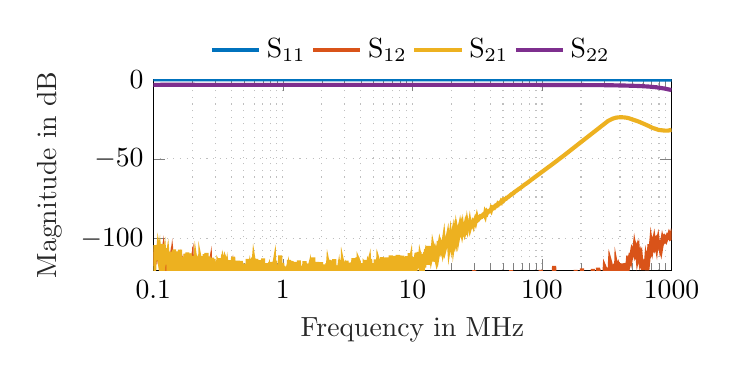
\begin{tikzpicture}

\begin{axis}[%
width=2.591in,
height=0.957in,
at={(0.616in,0.474in)},
scale only axis,
unbounded coords=jump,
xmode=log,
xmin=0.1,
xmax=1000,
xtick={0.1,1,10,100,1000},
xticklabels={{0.1},{1},{10},{100},{1000}},
xminorticks=true,
xlabel style={font=\color{white!15!black}},
xlabel={Frequency in MHz},
ymin=-120,
ymax=0,
ylabel style={font=\color{white!15!black}},
ylabel={Magnitude in dB},
axis background/.style={fill=white},
xmajorgrids,
xminorgrids,
ymajorgrids,
grid style={dotted},
legend style={at={(0.5,1.03)}, anchor=south, legend cell align=left, align=left, fill=none, draw=none},
legend columns = 4
]
\addplot [color=mycolor1, line width=1.5pt]
  table[row sep=crcr]{%
0.1	-0.127099897\\
0.104938455	-0.1141396679\\
0.147241545	-0.04110450823\\
0.161839461	-0.03905406293\\
0.176437377	-0.03071173398\\
0.190228728	-0.02477653598\\
0.207675395	-0.01833885628\\
0.237200526	-0.02174229824\\
0.250621039	-0.02096053274\\
0.313255351	-0.02292161943\\
0.337246194	-0.0243133435\\
0.479349732	-0.03624519116\\
0.785951488	-0.04785560216\\
0.873119539	-0.04592601041\\
0.986657469	-0.04243066091\\
1.100185548	-0.03943654928\\
1.393480989	-0.03487771218\\
1.802561859	-0.03160388964\\
2.144586756	-0.0259821635\\
2.720676423	-0.02145290545\\
3.192334481	-0.02040491718\\
4.413787719	-0.01945603712\\
4.68205492	-0.02089203318\\
4.947144752	-0.02112145525\\
6.751257296	-0.02206195948\\
10.29337529	-0.02728025888\\
20.76794004	-0.03445823109\\
120.8403675	-0.07229798331\\
158.4637493	-0.08092564516\\
194.394813	-0.09193614862\\
231.4289735	-0.1061567786\\
293.6641739	-0.1218397808\\
320.4307612	-0.1323223353\\
374.0873025	-0.1413890463\\
422.486007	-0.1571964398\\
463.9222374	-0.1606822091\\
487.6000834	-0.1732506386\\
514.2376601	-0.1836762096\\
540.8752369	-0.1763147414\\
561.5933521	-0.1762843592\\
621.6579634	-0.2037664539\\
658.2871889	-0.1923230783\\
678.6367587	-0.2027456071\\
711.1960703	-0.2219707422\\
772.2447796	-0.2119980179\\
815.7346424	-0.242697942\\
838.1916447	-0.234074211\\
866.2628976	-0.2273830553\\
939.248155	-0.2508877565\\
972.9336584	-0.2461726037\\
1001.004911	-0.2570104131\\
};
\addlegendentry{$\mathrm{S}_\mathrm{11}$}

\addplot [color=mycolor2, line width=1.5pt]
  table[row sep=crcr]{%
0.1	-110.8945728\\
0.100705494	-108.8999863\\
0.101410987	-115.5123151\\
0.102116481	-115.3903336\\
0.104938455	-105.6791173\\
0.105643948	-111.2823728\\
0.107054935	-106.8613124\\
0.108465922	-113.8544643\\
0.109171416	-105.2103276\\
0.109876909	-112.8949018\\
0.110582403	-108.0273542\\
0.11199339	-115.8848255\\
0.112698884	-109.1555032\\
0.113404377	-114.7009644\\
0.114815364	-111.8799785\\
0.116226351	-112.8945404\\
0.117637338	-110.1277251\\
0.118342832	-110.9943152\\
0.119048325	-109.5969508\\
0.119753819	-112.4027421\\
0.120459312	-110.9525647\\
0.121164806	-117.0406455\\
0.122575793	-107.6889616\\
0.123281287	-121.8105431\\
0.124692274	-113.6635901\\
0.125397767	-116.3079124\\
0.126103261	-108.2578004\\
0.127514248	-113.5040306\\
0.129630728	-109.5809745\\
0.131041715	-119.9861872\\
0.132452703	-111.7047394\\
0.133158196	-113.3019875\\
0.13386369	-108.5799556\\
0.134569183	-110.8529565\\
0.135274677	-120.4541386\\
0.13598017	-110.0446362\\
0.136685664	-114.0814341\\
0.137509601	-112.7378006\\
0.138482796	-114.1752059\\
0.13945599	-112.0817354\\
0.140429185	-114.6164861\\
0.141402379	-113.9982102\\
0.142375573	-114.0839984\\
0.143348768	-117.3973818\\
0.145295157	-108.6786291\\
0.147241545	-127.8660063\\
0.149187934	-111.3214411\\
0.150161129	-114.8437761\\
0.151134323	-111.655477\\
0.155027101	-119.6471333\\
0.156973489	-116.3475391\\
0.157946684	-117.5159262\\
0.158919878	-121.2993877\\
0.161839461	-110.9664776\\
0.162812656	-121.2123904\\
0.16378585	-112.8990414\\
0.164759045	-114.3254805\\
0.165732239	-119.5670413\\
0.166705433	-115.8617871\\
0.167678628	-116.7862392\\
0.168651822	-111.6513781\\
0.170598211	-123.6645423\\
0.171571405	-116.2842581\\
0.1725446	-116.7958514\\
0.173517794	-116.688243\\
0.174490989	-122.7634319\\
0.177410572	-113.8401718\\
0.178383766	-114.1894626\\
0.179356961	-116.7366886\\
0.180330155	-114.8544796\\
0.181303349	-119.6114546\\
0.183249738	-112.7757616\\
0.184222933	-126.7277425\\
0.186169321	-116.9277298\\
0.187142516	-129.3255726\\
nan	nan\\
0.1894048856	-132\\
0.191570779	-114.0195122\\
0.194254882	-118.9425248\\
0.198281036	-115.2060598\\
0.199623087	-129.440918\\
0.200965139	-115.8795393\\
0.20230719	-120.208224\\
0.203649241	-116.2396879\\
0.204991293	-117.622526\\
0.206333344	-116.6255479\\
0.207675395	-119.2362306\\
0.209017447	-118.1326838\\
0.210359498	-113.3469239\\
0.213043601	-126.5780505\\
0.214385652	-118.6451182\\
0.215727704	-120.5990217\\
0.218411806	-119.1486031\\
0.219753858	-114.3540231\\
0.221095909	-123.3482643\\
0.223780012	-116.4641811\\
0.225122063	-124.1286391\\
nan	nan\\
0.229148217	-121.6507926\\
0.23183232	-115.4721179\\
0.233174371	-116.2013383\\
0.234516423	-121.6573295\\
0.235858474	-116.3953218\\
0.239884628	-121.6990181\\
0.24122668	-113.9465035\\
0.242568731	-117.4723888\\
0.243910782	-115.877517\\
0.245252834	-124.5580785\\
0.247936937	-115.4015287\\
0.249278988	-123.0346447\\
0.250621039	-122.4088404\\
0.251963091	-117.2360684\\
0.253305142	-124.3376765\\
nan	nan\\
0.255989245	-121.5669155\\
0.257331296	-118.3142604\\
0.258673347	-130.4934475\\
0.261582765	-118.7570809\\
0.263428214	-123.5116884\\
0.265273664	-115.694484\\
0.268964563	-124.4560029\\
0.270810012	-117.3575214\\
0.272655462	-118.8155507\\
0.274500911	-117.4453383\\
0.276346361	-125.8540834\\
nan	nan\\
0.281882709	-124.236745\\
0.283728159	-117.385628\\
0.285573608	-121.3900221\\
nan	nan\\
0.298491755	-120.7738948\\
0.300337204	-119.1614047\\
0.302182654	-123.0797531\\
0.304028103	-121.7024078\\
0.305873553	-116.3652441\\
0.309564452	-129.8716996\\
0.311409901	-119.19042\\
0.313255351	-123.8402406\\
nan	nan\\
0.322482598	-120.4367129\\
0.324328048	-116.8642024\\
0.326173497	-120.3222958\\
nan	nan\\
0.333555295	-123.2532415\\
0.337246194	-114.6293512\\
0.339091643	-122.0583063\\
nan	nan\\
0.342782542	-125.2562673\\
0.344627992	-117.3040726\\
0.346473441	-130.4426021\\
nan	nan\\
0.35016434	-126.7392682\\
0.35200979	-119.3865447\\
0.353855239	-121.5281183\\
nan	nan\\
0.359701417	-125.528085\\
0.362247126	-117.6694324\\
0.364792835	-130.5824893\\
nan	nan\\
0.397887049	-121.5593802\\
0.402978467	-119.5570046\\
0.405524176	-124.1275819\\
0.408069885	-118.5480482\\
0.410615594	-124.2227886\\
0.413161302	-117.6458968\\
0.41825272	-125.0478973\\
0.420798429	-118.7519346\\
0.423344138	-129.1112468\\
nan	nan\\
0.430981264	-130.5608312\\
0.433526973	-119.4447226\\
0.436072682	-121.4102909\\
nan	nan\\
0.4844429756	-132\\
0.486986858	-117.2532432\\
0.489532567	-127.897799\\
0.492078276	-118.7237387\\
0.494623985	-131.5409315\\
nan	nan\\
0.551525082	-132\\
0.553774767	-118.9805336\\
0.557285342	-126.1073129\\
nan	nan\\
0.613454543	-130.3978553\\
0.616965118	-119.0656767\\
0.6194660038	-132\\
nan	nan\\
0.6451715524	-132\\
0.648560294	-119.6551674\\
0.6519307055	-132\\
nan	nan\\
0.819850175	-121.0807915\\
0.824692844	-119.2432791\\
0.829535514	-123.366729\\
nan	nan\\
1.466945464	-123.5633354\\
1.476128524	-119.7087955\\
1.481746206	-132\\
nan	nan\\
1.632240533	-125.1786002\\
1.641423592	-118.2688789\\
1.650606652	-131.1220306\\
nan	nan\\
3.695113077	-132\\
3.717170002	-119.0327023\\
3.741191303	-129.3066525\\
nan	nan\\
5.676141789	-125.5189023\\
5.709278018	-117.4829947\\
5.742414247	-131.6741793\\
nan	nan\\
6.073776536	-124.1712465\\
6.106912765	-119.7076561\\
6.140048994	-128.4743622\\
nan	nan\\
29.89367462	-122.0403042\\
30.05856234	-119.8468083\\
30.22345006	-128.522137\\
nan	nan\\
57.45208531	-127.366735\\
57.76475867	-119.7789088\\
58.07743202	-124.3363732\\
nan	nan\\
97.39448	-127.5963812\\
97.98927454	-119.5644021\\
98.38342476	-132\\
nan	nan\\
123.2940663	-122.90821\\
124.1119659	-117.1476685\\
124.9298655	-123.304689\\
nan	nan\\
180.8557749	-123.5023528\\
181.9840281	-119.6330571\\
183.1122813	-130.2733401\\
nan	nan\\
202.2925852	-127.9183141\\
203.4208383	-118.6578478\\
204.4494035	-132\\
nan	nan\\
245.4318936	-125.4863605\\
246.9877736	-119.003075\\
248.5436536	-131.7351146\\
nan	nan\\
268.7700937	-127.8153768\\
270.3259737	-118.244114\\
271.8818538	-126.7027597\\
273.4377338	-119.0079526\\
274.9467361	-132\\
nan	nan\\
303.260668	-122.7991199\\
305.4069296	-118.2803743\\
307.5531913	-118.8709334\\
309.6994529	-121.9713469\\
nan	nan\\
316.1382379	-129.3502383\\
318.2844995	-118.2266556\\
320.4307612	-123.2086745\\
nan	nan\\
331.1620695	-124.240991\\
335.4545928	-114.5985772\\
337.6008544	-115.4165471\\
339.7471161	-127.3654714\\
nan	nan\\
356.9172093	-128.5953595\\
359.0634709	-118.3115346\\
361.2097326	-118.4764503\\
363.3559942	-126.2901178\\
367.6485175	-115.7456816\\
369.7947792	-131.395343\\
374.0873025	-117.0177816\\
376.2335641	-118.1021231\\
378.3798258	-117.724167\\
380.5260874	-125.4071164\\
382.6723491	-123.832625\\
384.8186107	-114.6474146\\
386.9648724	-118.4069087\\
389.1111341	-117.1775679\\
391.2573957	-117.4708416\\
393.4036574	-117.2450193\\
395.549919	-117.638712\\
397.6961807	-123.7888055\\
nan	nan\\
401.988704	-120.386054\\
404.1349656	-119.4693284\\
408.4274889	-115.5013596\\
410.5737506	-121.9706499\\
414.8662739	-117.721001\\
417.0125355	-125.7892626\\
422.486007	-116.8055872\\
425.4457377	-116.7496507\\
428.4054685	-126.9308617\\
431.3651992	-116.9532716\\
434.32493	-120.7854524\\
437.2846607	-117.9081338\\
440.2443915	-125.7469109\\
nan	nan\\
452.0833145	-122.0657831\\
460.9625067	-113.3274376\\
463.9222374	-113.5405419\\
466.8819682	-115.1113541\\
469.8416989	-113.6631589\\
472.8014297	-113.971176\\
481.6806219	-110.4253584\\
484.6403527	-110.4934195\\
487.6000834	-111.6103372\\
496.4792757	-107.9833767\\
499.4390064	-108.4798338\\
502.3987372	-108.4537779\\
505.3584679	-107.2041371\\
508.3181987	-107.3853321\\
511.2779294	-107.2902458\\
514.2376601	-107.8169241\\
517.1973909	-106.0959964\\
520.1571216	-107.4136401\\
526.0765831	-105.7768588\\
531.9960446	-107.184597\\
534.9557754	-106.6952109\\
537.9155061	-107.6381796\\
540.8752369	-106.999429\\
546.7946984	-111.3199584\\
552.7141599	-109.5236167\\
555.6738906	-112.0353094\\
558.6336214	-108.6031181\\
561.5933521	-108.7799194\\
570.4725443	-112.5911116\\
573.4322751	-111.808074\\
576.8889099	-113.3440778\\
580.9588239	-112.4167085\\
589.0986518	-117.882931\\
593.1685657	-114.244378\\
597.2384797	-114.8327569\\
605.3783076	-119.6583609\\
613.5181355	-114.8420297\\
617.5880494	-114.8696184\\
621.6579634	-119.3185404\\
625.7278773	-113.0559169\\
629.7977913	-116.6848576\\
633.8677052	-116.6692229\\
637.9376192	-113.5804698\\
642.0075331	-114.6709662\\
650.147361	-119.7004757\\
662.3571029	-113.265782\\
674.5668447	-105.1391002\\
678.6367587	-105.2227167\\
682.7066726	-105.4879264\\
686.7765866	-103.5313454\\
690.8465005	-106.1392367\\
694.9164145	-103.8074336\\
698.9863284	-105.2649035\\
703.0562424	-104.4464023\\
707.1261564	-105.4836976\\
715.2659843	-102.9179984\\
723.4058122	-103.9847742\\
731.5456401	-101.9301874\\
735.615554	-103.5243212\\
747.8252959	-102.2663208\\
751.8952098	-103.8849622\\
760.0350377	-102.8592113\\
764.1049517	-103.9181291\\
768.1748656	-101.9662299\\
772.2447796	-102.0134497\\
780.3846075	-102.8570756\\
784.4545214	-101.9676656\\
788.5244354	-103.5037373\\
793.2776401	-102.9321956\\
798.8918907	-103.5096266\\
804.5061413	-103.4009618\\
810.1203919	-103.756959\\
815.7346424	-103.5537387\\
821.348893	-105.1565434\\
826.9631436	-104.2830965\\
832.5773941	-105.5674525\\
849.4201459	-101.2746218\\
855.0343964	-102.3029075\\
877.4913987	-99.85205156\\
883.1056493	-100.237214\\
888.7198998	-99.65643098\\
905.5626516	-100.7439009\\
916.7911527	-99.4286625\\
922.4054033	-99.46293204\\
928.0196538	-98.88750627\\
939.248155	-99.52903262\\
944.8624056	-99.45149585\\
961.7051573	-97.32033667\\
972.9336584	-98.12781637\\
984.1621595	-99.78349699\\
989.7764101	-99.68918382\\
995.3906607	-98.77690925\\
1001.004911	-99.49465895\\
};
\addlegendentry{$\mathrm{S}_\mathrm{12}$}

\addplot [color=mycolor3, line width=1.5pt]
  table[row sep=crcr]{%
0.1	-111.0725621\\
0.100705494	-108.629415\\
0.101410987	-121.062915\\
0.102821974	-104.0430506\\
0.103527468	-112.1054398\\
0.104938455	-106.4412834\\
0.106349442	-110.9114466\\
0.107054935	-110.5069654\\
0.107760429	-104.6829407\\
0.108465922	-111.1189162\\
0.109171416	-108.1054576\\
0.110582403	-111.3012897\\
0.111287897	-109.7053929\\
0.11199339	-112.769548\\
0.112698884	-110.9141386\\
0.113404377	-115.834062\\
0.114109871	-105.6613144\\
0.114815364	-121.6625922\\
0.115520858	-106.8781527\\
0.116931845	-111.515925\\
0.117637338	-103.3623619\\
0.119048325	-123.3982798\\
0.120459312	-110.1959261\\
0.121164806	-113.2640607\\
0.1218703	-111.8034947\\
0.122575793	-115.1050912\\
0.123281287	-105.9471859\\
0.124692274	-116.3054546\\
0.125397767	-108.9141517\\
0.126103261	-111.3097349\\
0.126808754	-107.3344031\\
0.127514248	-112.1928642\\
0.128219741	-112.079717\\
0.128925235	-110.8926047\\
0.129630728	-113.3351182\\
0.130336222	-109.8160867\\
0.131041715	-124.1873526\\
0.132452703	-112.4269618\\
0.133158196	-117.4954191\\
0.13386369	-110.558165\\
0.134569183	-120.7305006\\
0.135274677	-110.4159569\\
0.13598017	-121.4654054\\
0.138482796	-108.1872709\\
0.13945599	-122.8548283\\
0.141402379	-109.1353732\\
0.142375573	-113.6820332\\
0.143348768	-113.3173604\\
0.144321962	-106.8771505\\
0.147241545	-114.2332403\\
0.14821474	-110.4960727\\
0.149187934	-120.6612152\\
0.150161129	-118.2558291\\
0.151134323	-108.0351931\\
0.152107517	-130.4324033\\
0.155027101	-113.1547233\\
0.156000295	-108.9947276\\
0.159893073	-118.9378477\\
0.160866267	-106.814206\\
0.161839461	-125.1142171\\
0.162812656	-115.305865\\
0.16378585	-123.530112\\
0.165732239	-115.9098547\\
0.167678628	-129.3436437\\
0.168651822	-111.3965439\\
0.170598211	-123.1680154\\
0.1725446	-111.8908344\\
0.174490989	-126.2043284\\
0.177410572	-109.5056336\\
0.178383766	-112.8361691\\
0.179356961	-127.838515\\
0.180330155	-113.3340666\\
0.181303349	-114.6384783\\
0.182276544	-113.9322499\\
0.183249738	-108.6583781\\
0.185196127	-118.153841\\
0.186169321	-114.963805\\
0.187142516	-122.6866097\\
0.190228728	-109.31266\\
0.191570779	-110.9192929\\
0.194254882	-118.8073331\\
0.195596933	-114.3404825\\
0.196938984	-122.5119689\\
0.198281036	-111.9793783\\
0.200965139	-131.3830968\\
0.20230719	-110.764507\\
0.203649241	-113.6087503\\
0.204991293	-122.1473721\\
0.209017447	-114.2773733\\
0.210359498	-117.0771509\\
0.21170155	-113.7361856\\
0.214385652	-116.7822018\\
0.215727704	-116.1878809\\
0.217069755	-120.1335788\\
nan	nan\\
0.221095909	-124.9946507\\
0.22243796	-112.0651901\\
0.223780012	-126.7855224\\
nan	nan\\
0.226464115	-120.0843461\\
0.227806166	-118.0661416\\
0.229148217	-130.3619597\\
0.230490269	-114.3285788\\
0.23183232	-115.3839969\\
0.233174371	-113.0391991\\
0.235858474	-129.9467895\\
0.237200526	-113.8273895\\
0.2385023304	-132\\
nan	nan\\
0.2385994336	-132\\
0.242568731	-115.4006685\\
0.243910782	-110.9831013\\
0.245252834	-115.3014701\\
0.246594885	-112.4293207\\
0.247936937	-116.0933298\\
0.249278988	-109.6606236\\
0.250621039	-113.111921\\
0.251963091	-113.0595707\\
0.253305142	-114.8792014\\
0.254647193	-122.8173427\\
0.257331296	-108.9451615\\
0.258673347	-129.7578791\\
0.261582765	-115.9705281\\
0.2632934871	-132\\
nan	nan\\
0.263811826	-132\\
0.267119113	-111.0922485\\
0.270810012	-124.5798591\\
0.272655462	-119.1172238\\
0.274500911	-124.720138\\
0.28003726	-112.5255783\\
0.281882709	-115.3218889\\
0.283728159	-111.9527727\\
0.285573608	-130.4714068\\
0.287419058	-119.1803544\\
0.289264507	-120.7387844\\
0.291109957	-112.7411406\\
0.292955406	-117.486955\\
0.296646305	-114.282227\\
0.300337204	-124.450888\\
0.302182654	-117.7375276\\
0.304028103	-123.8437201\\
0.305873553	-115.5651451\\
0.309564452	-120.8365459\\
0.311409901	-114.6143265\\
0.313255351	-126.9003311\\
0.31694625	-115.4610336\\
0.318791699	-115.8765089\\
0.320637149	-127.7782122\\
0.322482598	-119.1119705\\
0.326173497	-128.274212\\
0.328018947	-112.2683681\\
0.331709845	-126.1258791\\
0.333555295	-118.5451745\\
0.335400744	-125.0427861\\
0.340937093	-117.4193742\\
0.342782542	-118.1630028\\
0.344627992	-123.1365429\\
0.346473441	-119.8264117\\
0.348318891	-122.5844079\\
0.35016434	-114.9179872\\
0.35200979	-115.5214473\\
0.353855239	-112.9084246\\
0.355700689	-118.7649652\\
0.357546138	-115.0894121\\
0.362247126	-127.9483287\\
0.364792835	-115.0752251\\
0.367338544	-115.7672368\\
0.369884252	-122.1850761\\
0.372429961	-119.8760377\\
0.37497567	-121.9169621\\
0.377521379	-115.9309288\\
0.382612797	-120.2710699\\
nan	nan\\
0.390249923	-125.5597241\\
0.392795632	-113.4766054\\
0.395341341	-115.5738513\\
0.3974498366	-132\\
nan	nan\\
0.408069885	-123.1452755\\
0.413161302	-111.30669\\
0.41825272	-120.6265676\\
nan	nan\\
0.423344138	-122.6756805\\
0.425889847	-117.3698154\\
0.433526973	-123.7826912\\
0.436072682	-118.5831527\\
0.438618391	-124.3749881\\
0.441164099	-117.5609145\\
0.443709808	-117.8522422\\
0.446255517	-120.3517299\\
0.448801226	-113.838247\\
0.451346935	-123.1268737\\
nan	nan\\
0.46152977	-123.407337\\
0.464075479	-119.4525094\\
0.466621188	-130.6051635\\
0.474258314	-113.8905574\\
0.476804023	-120.9467946\\
nan	nan\\
0.486986858	-121.745132\\
0.489532567	-116.2392559\\
0.494623985	-119.0436128\\
0.497605565	-115.7233489\\
0.504626715	-121.2886353\\
nan	nan\\
0.518669016	-127.6408118\\
0.522179591	-116.0734322\\
0.5248705721	-132\\
nan	nan\\
0.5266147484	-132\\
0.529200741	-118.5230493\\
0.532711316	-123.5753633\\
0.536221891	-112.6928735\\
0.543243041	-120.2889682\\
0.550264191	-115.0369349\\
0.553774767	-123.7482136\\
nan	nan\\
0.560795917	-124.0836669\\
0.564306492	-119.9683524\\
0.567817067	-120.9666956\\
0.571327642	-117.6017169\\
0.574838217	-117.9602011\\
0.578348792	-112.7225025\\
0.581859367	-131.5962724\\
0.585369942	-119.1917849\\
0.588880517	-119.878336\\
0.595901667	-114.4614375\\
0.599412243	-115.8253962\\
0.606433393	-124.5351055\\
0.613454543	-115.7965277\\
0.616965118	-119.4829656\\
0.623986268	-112.6546381\\
0.631007418	-122.1546071\\
0.638028568	-114.5405463\\
0.645049719	-126.7487755\\
0.652070869	-118.7688267\\
0.655581444	-124.8677942\\
0.659092019	-113.5450915\\
0.669623744	-124.2241937\\
nan	nan\\
0.6994030959	-132\\
0.703626107	-112.3105343\\
0.7082265282	-132\\
nan	nan\\
0.7087982535	-132\\
0.713311446	-117.8945893\\
0.722996785	-129.2158674\\
0.732682124	-115.7089745\\
0.737524793	-123.9463032\\
0.742367463	-115.3241721\\
0.747210132	-124.3458302\\
0.756895471	-115.8390481\\
0.76658081	-120.1092449\\
0.77142348	-119.4659995\\
0.776266149	-123.9737691\\
nan	nan\\
0.790794158	-124.7141124\\
0.800479497	-114.6918847\\
0.810164836	-123.9069306\\
0.819850175	-114.6616975\\
0.824692844	-120.2496622\\
0.829535514	-119.9308841\\
0.834378183	-122.8124865\\
0.8371283795	-132\\
nan	nan\\
0.8406133133	-132\\
0.844063522	-114.7793117\\
0.848906192	-118.6035538\\
0.858591531	-116.2490432\\
0.8634342	-121.7400539\\
0.873119539	-113.7515891\\
0.8850323387	-132\\
nan	nan\\
0.8899938494	-132\\
0.897332887	-119.2099641\\
0.902175556	-122.9619166\\
0.907018226	-118.167722\\
0.916703565	-121.4064483\\
nan	nan\\
0.926388904	-127.5205945\\
0.931231573	-116.1646738\\
0.936074243	-120.9036191\\
nan	nan\\
0.9490344433	-132\\
0.953266857	-110.5586049\\
0.95994498	-125.8005964\\
0.966623102	-117.5662662\\
0.973301224	-117.7820483\\
0.979979347	-118.9975485\\
0.986657469	-115.2410963\\
1.000013714	-119.5525583\\
1.006691836	-117.1126659\\
1.013369958	-126.5529136\\
1.02004808	-117.5718417\\
1.026726203	-127.5402484\\
1.033404325	-119.4371758\\
1.040082447	-125.2674917\\
nan	nan\\
1.053438692	-128.1850359\\
1.060116814	-118.1344512\\
1.066794937	-121.4016622\\
1.080151181	-119.7758734\\
1.086829304	-127.9863948\\
nan	nan\\
1.10686367	-131.2134739\\
1.113541793	-113.3080697\\
1.126898037	-124.5805777\\
1.140254282	-116.2017547\\
1.146932404	-117.9239112\\
1.153610527	-117.4911851\\
1.166966771	-114.049074\\
1.173141772	-132\\
nan	nan\\
1.175693205	-132\\
1.187001138	-118.3230481\\
1.200357383	-120.6406267\\
1.207035505	-118.2838336\\
1.213713627	-121.1022062\\
1.22039175	-120.5161813\\
1.227069872	-114.6372411\\
1.233747994	-121.5816006\\
1.240426117	-116.8655731\\
1.247104239	-121.4666901\\
1.253782361	-116.2911378\\
1.260460484	-119.087934\\
1.267138606	-117.1078625\\
1.273816728	-119.8990821\\
1.28049485	-117.1970084\\
1.287172973	-122.8019706\\
nan	nan\\
1.320016515	-122.0054717\\
1.329199574	-113.6672483\\
1.338382633	-124.8084204\\
nan	nan\\
1.365931811	-125.2758731\\
1.375114871	-116.9863548\\
1.38429793	-119.1208409\\
1.393480989	-126.5792163\\
1.402664049	-124.600316\\
1.411847108	-116.9992968\\
1.421030167	-123.2948076\\
1.430213227	-119.1210017\\
1.439396286	-122.8748609\\
nan	nan\\
1.457762405	-121.1273115\\
1.466945464	-114.1027987\\
1.476128524	-121.0463328\\
1.485311583	-115.3009389\\
1.494494642	-120.6737327\\
nan	nan\\
1.52204382	-122.5153036\\
1.540409939	-115.6907706\\
1.549592999	-118.3619893\\
1.558776058	-116.4384417\\
1.567959117	-131.9323128\\
1.577142177	-118.1387801\\
1.586325236	-119.8822599\\
1.595508295	-119.072515\\
1.604691355	-126.8324921\\
1.613874414	-118.1239476\\
1.624355056	-132\\
1.650606652	-115.7677415\\
1.659789711	-124.2840904\\
1.66897277	-122.908297\\
1.67815583	-117.1863606\\
1.687338889	-119.0965009\\
1.691003885	-132\\
nan	nan\\
1.701992827	-132\\
1.714888067	-111.7119547\\
1.733254186	-125.775763\\
1.742437245	-118.9675967\\
1.751620305	-123.6545883\\
1.769986423	-115.0305718\\
1.78989427	-120.2351816\\
1.802561859	-115.1240055\\
1.815229447	-122.4330707\\
1.840564625	-114.561823\\
1.853232214	-123.0824422\\
nan	nan\\
1.878567391	-131.91433\\
1.89123498	-116.258536\\
1.899764604	-132\\
nan	nan\\
1.961805672	-132\\
1.967240513	-114.6556773\\
1.979908101	-127.6584979\\
nan	nan\\
2.017910868	-124.6798765\\
2.030578457	-119.5015147\\
2.043246045	-121.6324171\\
2.055913634	-116.2270047\\
2.081248812	-120.6004651\\
2.095293905	-132\\
2.106583989	-116.4016293\\
2.131919167	-120.4471012\\
2.144586756	-118.7530654\\
2.157254344	-131.8762868\\
nan	nan\\
2.182589522	-127.9846455\\
2.207924699	-115.4130015\\
2.220592288	-119.5412647\\
2.233259877	-116.3227782\\
2.258595054	-118.239042\\
2.271262643	-113.2558186\\
2.283930232	-121.0866434\\
2.296597821	-120.1427755\\
2.30926541	-115.4698299\\
2.321932998	-117.8785128\\
2.334600587	-114.7307633\\
2.347268176	-126.7637753\\
2.372603353	-113.6592322\\
2.385270942	-115.3312792\\
2.397938531	-126.5757775\\
2.41060612	-114.4891653\\
2.423273708	-115.6699698\\
2.437653359	-132\\
2.461276475	-116.5990555\\
2.476112985	-118.3630347\\
2.493581802	-112.9397612\\
2.511050619	-121.9302031\\
nan	nan\\
2.580925887	-123.4096756\\
2.615863521	-117.7106186\\
2.633332338	-122.1403166\\
2.668269972	-116.8794942\\
2.685738789	-120.8181254\\
2.703207606	-119.4302302\\
2.73814524	-123.6033683\\
2.755614057	-113.3661005\\
2.773082874	-123.1771738\\
2.790551691	-118.2639615\\
2.808020508	-124.3998673\\
nan	nan\\
2.877895776	-124.8255672\\
2.895364593	-115.9535905\\
2.91283341	-116.9451961\\
2.930302227	-124.1905267\\
2.965239861	-114.349989\\
2.982708678	-127.6548903\\
3.000177495	-114.4317265\\
3.035115129	-127.4738935\\
3.070052763	-115.1595956\\
3.087521579	-119.1765492\\
3.104990396	-113.8252501\\
3.122459213	-124.0324147\\
3.13992803	-117.7937262\\
3.157396847	-118.1305839\\
3.174865664	-123.445926\\
3.209803298	-117.3548984\\
3.227272115	-119.3417608\\
3.244740932	-115.0627038\\
3.297147383	-122.2755114\\
nan	nan\\
3.332085017	-126.2730887\\
3.367022651	-118.6693957\\
3.384491468	-126.6220804\\
3.428914395	-114.960051\\
3.476956996	-127.2578998\\
3.500978297	-112.1473832\\
3.524999597	-129.3265106\\
3.549020898	-115.4226027\\
3.573042199	-122.6617148\\
nan	nan\\
3.669127401	-122.148543\\
3.693148702	-112.2627575\\
3.717170002	-117.3629527\\
3.765212603	-111.8176693\\
3.789233904	-114.2309762\\
3.813255204	-129.2440629\\
3.837276505	-114.0617783\\
3.861297806	-114.5851957\\
3.885319106	-121.1927474\\
3.909340407	-116.7802648\\
3.933361707	-128.1525206\\
3.957383008	-119.2700137\\
3.981404309	-122.1132507\\
4.02944691	-117.7863135\\
4.05346821	-124.9991933\\
4.077489511	-119.9610512\\
4.125532112	-128.7087659\\
4.149553413	-115.3640259\\
4.173574713	-120.3162574\\
nan	nan\\
4.245638615	-121.6295395\\
4.269659915	-116.4354054\\
4.293681216	-116.7445754\\
4.317702517	-121.4579789\\
4.389766418	-113.442687\\
4.46183032	-130.7685522\\
4.533894222	-113.3593993\\
4.557915522	-117.0969458\\
4.581936823	-115.4096983\\
4.605958124	-115.7869906\\
4.629979424	-115.0752869\\
4.654000725	-119.1716682\\
4.68205492	-118.0885963\\
4.715191149	-112.7648436\\
4.781463607	-123.7624762\\
4.814599836	-115.3882106\\
4.847736065	-126.2402199\\
4.947144752	-116.8904047\\
4.980280981	-121.3862539\\
nan	nan\\
5.179098354	-120.6370934\\
5.212234583	-113.0815521\\
5.245370812	-117.5371458\\
5.278507041	-114.3724502\\
5.31164327	-124.2684795\\
nan	nan\\
5.377915728	-126.3736556\\
5.444188186	-114.0710637\\
5.477324415	-114.7771943\\
5.510460644	-122.0169763\\
nan	nan\\
5.580264426	-132\\
5.609869331	-116.7863111\\
5.64300556	-125.1379757\\
5.676141789	-116.916099\\
5.709278018	-118.2694675\\
5.742414247	-114.2888942\\
5.775550475	-123.1735522\\
5.808686704	-121.5277897\\
5.841822933	-111.5687908\\
5.94123162	-126.1956753\\
5.974367849	-115.7641741\\
6.007504078	-122.0417279\\
6.040640307	-121.4101759\\
6.106912765	-112.2507917\\
6.173185223	-125.8213363\\
6.239457681	-115.1075451\\
6.27259391	-123.6027146\\
6.305730139	-113.256531\\
6.338866368	-117.6060849\\
6.372002597	-111.6935501\\
6.405138826	-119.4734804\\
6.438275055	-114.7467217\\
6.477084809	-114.8918035\\
6.522780223	-112.8941049\\
6.659866467	-128.5518768\\
6.705561881	-114.0196211\\
6.751257296	-120.4559065\\
6.79695271	-110.5560692\\
6.888343539	-119.133591\\
6.979734368	-112.4756486\\
7.025429782	-118.4899323\\
7.116820611	-110.8259713\\
7.162516026	-121.8660888\\
nan	nan\\
7.35100666	-132\\
7.390993098	-112.9286464\\
7.439283819	-132\\
7.482383927	-114.2622425\\
7.528079341	-124.2624342\\
7.573774756	-117.5399709\\
7.665165585	-126.6525818\\
7.710860999	-110.2460393\\
7.802251828	-116.3811472\\
7.847947242	-114.2044824\\
7.939338071	-118.6457243\\
7.985033486	-112.3264247\\
8.0307289	-124.3425921\\
8.122119729	-113.8842721\\
8.213510558	-120.4489952\\
8.259205972	-111.9398758\\
8.304901387	-116.1085016\\
8.350596801	-110.590609\\
8.396292216	-122.5553786\\
8.487683044	-115.291388\\
8.533378459	-118.4862273\\
8.624769288	-111.589311\\
8.716160117	-130.1566002\\
8.761855531	-112.5701091\\
8.85324636	-119.925011\\
8.906613499	-118.1498888\\
8.969648125	-127.602159\\
9.095717379	-110.9864325\\
9.158752005	-116.3275314\\
9.221786632	-114.2619068\\
9.347855886	-124.6570664\\
nan	nan\\
9.473925139	-125.165367\\
9.536959766	-109.1483388\\
9.599994392	-115.3507806\\
9.663029019	-114.2347376\\
9.726063646	-120.5723268\\
9.789098272	-117.8246681\\
9.852132899	-124.2280873\\
9.915167526	-122.8855134\\
9.978202153	-111.4988865\\
10.04123678	-117.1559378\\
10.16730603	-111.728839\\
10.23034066	-118.684459\\
10.29337529	-111.9992233\\
10.35640991	-116.5059844\\
10.41944454	-116.1390273\\
10.48247917	-117.5436324\\
10.54551379	-122.4384414\\
10.67158305	-113.5390429\\
10.73461767	-113.9271972\\
10.92372155	-108.8157028\\
11.11282543	-118.6044901\\
11.17586006	-108.3423329\\
11.30192931	-112.6938382\\
11.36496394	-108.4955206\\
11.42799857	-115.0167418\\
11.49103319	-112.1609311\\
11.55406782	-112.9900815\\
11.61710245	-122.7169917\\
11.80620633	-109.7656899\\
11.86924095	-116.3108366\\
11.93227558	-115.1199118\\
11.99531021	-122.5677686\\
12.18441409	-111.2668195\\
12.32127602	-118.0775111\\
12.40820182	-109.4250476\\
12.49512763	-112.9389289\\
12.58205343	-108.3294096\\
12.66897924	-111.2952296\\
12.75590504	-106.4427472\\
12.84283085	-110.5542407\\
12.92975665	-108.0910171\\
13.01668246	-108.5161632\\
13.10360827	-113.8102952\\
13.19053407	-104.558335\\
13.27745988	-116.3995323\\
13.36438568	-113.8724887\\
13.45131149	-104.5408492\\
13.53823729	-110.3034031\\
13.7120889	-106.8319053\\
13.79901471	-113.3895089\\
13.88594051	-109.383612\\
13.97286632	-111.1760293\\
14.05979212	-110.1379585\\
14.14671793	-113.3689769\\
14.40749535	-105.5813782\\
14.58134696	-107.4601578\\
14.66827276	-114.3440966\\
15.01597599	-109.4269532\\
15.10290179	-110.4027\\
15.36367921	-104.4630825\\
15.45060501	-112.2168411\\
15.62445662	-106.8617311\\
15.71138243	-109.8398146\\
15.79830823	-108.8938198\\
15.97215985	-101.4407337\\
16.05908565	-105.5401954\\
16.23293726	-103.2692051\\
16.49371468	-105.6018075\\
16.58064048	-104.7084647\\
16.75449209	-106.0727113\\
16.8414179	-103.6312936\\
16.94293753	-107.2644944\\
17.06246886	-102.8136524\\
17.18200019	-104.9821315\\
17.42106284	-101.77444\\
17.54059417	-105.2688925\\
17.6601255	-104.2936148\\
17.77965683	-104.3118489\\
17.89918816	-100.6067856\\
18.01871949	-104.3305834\\
18.13825081	-103.3853567\\
18.25778214	-103.5674642\\
18.61637613	-100.0447871\\
18.73590746	-103.4599795\\
18.85543878	-99.19877976\\
18.97497011	-101.0705439\\
19.09450144	-100.3870603\\
19.21403277	-103.9961677\\
19.57262676	-99.51163595\\
19.69215808	-101.8938958\\
19.81168941	-98.21861781\\
19.93122074	-102.4049341\\
20.05075207	-98.97871556\\
20.1702834	-101.6299354\\
20.40934606	-99.1202045\\
20.52887738	-102.4331673\\
20.64840871	-98.77402576\\
20.76794004	-102.0281588\\
21.0070027	-99.19773193\\
21.12653403	-100.1900266\\
21.36559668	-96.77887712\\
21.60465934	-98.87423858\\
21.72419067	-96.70508007\\
21.843722	-98.19207142\\
21.96325333	-96.78004154\\
22.08278466	-97.98467288\\
22.56090997	-95.42203612\\
22.6804413	-98.01337466\\
23.03903528	-94.96811137\\
23.15856661	-97.2788423\\
23.62794129	-95.88068239\\
23.79282901	-96.34274061\\
23.95771673	-94.30843937\\
24.12260445	-95.54859244\\
24.28749216	-94.08872173\\
24.45237988	-96.21665623\\
24.6172676	-95.77237825\\
24.78215532	-94.3226077\\
25.11193076	-95.6727798\\
25.4417062	-93.32609718\\
25.60659392	-95.06259713\\
26.10125708	-93.0494217\\
26.2661448	-93.67395792\\
26.43103252	-91.77347248\\
26.59592024	-93.13846943\\
26.92569567	-92.12720498\\
27.09058339	-92.19121658\\
27.58524655	-92.74031552\\
27.75013427	-91.30339369\\
27.91502199	-92.69461109\\
28.24479743	-91.21522701\\
28.40968515	-91.36885029\\
28.57457287	-90.72515514\\
28.90434831	-91.28369306\\
29.23412375	-90.27796573\\
29.39901147	-90.82367405\\
29.56389918	-89.57072981\\
30.05856234	-90.18335001\\
30.22345006	-90.07290853\\
30.5532255	-88.70799507\\
30.71811322	-89.28103138\\
30.88300094	-88.45544996\\
31.21277638	-88.8893325\\
31.3776641	-88.61869582\\
31.54255182	-87.64453498\\
31.70743954	-88.41828841\\
31.87232726	-88.22468043\\
32.03721498	-88.24514737\\
32.68510032	-87.50156525\\
33.3672491	-86.25991171\\
33.82201495	-86.59343786\\
34.04939788	-86.50145342\\
34.50416373	-85.62583309\\
34.73154665	-85.65573911\\
34.95892958	-85.31162334\\
35.1863125	-85.44708182\\
35.41369543	-85.43881261\\
35.86846128	-84.58916887\\
36.0958442	-84.62813587\\
36.32322713	-85.17551118\\
36.55061005	-83.86082438\\
36.77799298	-84.29739821\\
37.23275883	-83.87370426\\
37.46014176	-84.10865913\\
37.68752468	-83.43608287\\
37.91490761	-83.74842254\\
40.18873686	-81.78691887\\
40.41611978	-82.11233936\\
40.64350271	-81.35044614\\
40.87088564	-81.68139144\\
41.55303441	-80.77521149\\
41.78041734	-80.89717947\\
42.23518319	-80.44369554\\
42.46256611	-80.56950266\\
43.14471489	-79.9198282\\
43.37209781	-80.13880058\\
44.05424659	-79.40806373\\
44.31980444	-79.4856444\\
44.6324778	-79.07042887\\
44.94515115	-79.12800313\\
45.2578245	-78.85104949\\
45.57049786	-78.89513346\\
45.88317121	-78.18874458\\
46.19584457	-78.37941459\\
46.82119127	-78.19024196\\
48.07188469	-77.02709144\\
48.38455805	-77.20851591\\
48.6972314	-76.56202793\\
49.00990475	-76.77296051\\
49.32257811	-76.70978137\\
49.94792482	-76.1081708\\
50.26059817	-76.17546437\\
50.57327152	-75.67376364\\
50.88594488	-75.80884693\\
52.44931165	-74.9514389\\
52.761985	-74.96309292\\
53.38733171	-74.36778833\\
53.70000506	-74.3991561\\
54.63802513	-74.0087497\\
58.07743202	-72.20694965\\
58.39010537	-72.24490006\\
60.2661455	-71.29061645\\
60.57881885	-71.30725838\\
61.37530425	-70.8343537\\
66.55111852	-68.70559465\\
66.98243637	-68.67991444\\
69.13902565	-67.82263487\\
73.88352206	-65.96741542\\
74.74615777	-65.79871541\\
77.3340649	-64.91696509\\
83.37251487	-62.88322348\\
84.90379459	-62.42454902\\
122.4761667	-52.85752598\\
137.1983596	-49.8200802\\
142.1057572	-48.8809135\\
148.648954	-47.68268729\\
195.5230661	-40.09436936\\
322.5770228	-26.30070391\\
350.4784243	-24.79957383\\
371.9410408	-24.16519557\\
386.9648724	-23.96070837\\
399.8424423	-23.89353435\\
406.2812273	-23.88581138\\
414.8662739	-23.89586813\\
431.3651992	-23.97847956\\
449.1235837	-24.1577257\\
466.8819682	-24.46572867\\
517.1973909	-25.68361497\\
558.6336214	-26.61999978\\
633.8677052	-28.55909978\\
658.2871889	-29.15951853\\
715.2659843	-30.56260076\\
751.8952098	-31.13958541\\
798.8918907	-31.86545974\\
832.5773941	-32.00261856\\
860.648647	-32.14753172\\
888.7198998	-32.24391589\\
922.4054033	-32.28226813\\
939.248155	-32.23749082\\
1001.004911	-31.7884442\\
};
\addlegendentry{$\mathrm{S}_\mathrm{21}$}

\addplot [color=mycolor4, line width=1.5pt]
  table[row sep=crcr]{%
0.1	-3.575559904\\
0.106349442	-3.561407016\\
0.123281287	-3.52894133\\
0.142375573	-3.525420595\\
0.152107517	-3.524599159\\
0.198281036	-3.544435303\\
0.265273664	-3.560600156\\
0.281882709	-3.562272872\\
0.348318891	-3.572585841\\
0.560795917	-3.581744803\\
0.926388904	-3.575005621\\
1.240426117	-3.56461313\\
1.485311583	-3.56501472\\
1.954572924	-3.557413428\\
4.581936823	-3.552835412\\
6.477084809	-3.552165132\\
10.16730603	-3.5540156\\
60.2661455	-3.578899161\\
76.47142919	-3.591122517\\
112.2643436	-3.620736495\\
160.5472178	-3.657498497\\
185.3687876	-3.681648072\\
273.4377338	-3.748012893\\
299.8876939	-3.763000377\\
316.1382379	-3.784031996\\
348.3321627	-3.842167236\\
446.163853	-4.025120151\\
514.2376601	-4.176413789\\
549.7544291	-4.255245855\\
593.1685657	-4.394420697\\
662.3571029	-4.613231963\\
768.1748656	-5.113971938\\
883.1056493	-5.884109441\\
1001.004911	-6.826575589\\
};
\addlegendentry{$\mathrm{S}_\mathrm{22}$}

\end{axis}
\end{tikzpicture}%
	\caption{VNA measurement of high-pass of active current shunt.}\label{fig:VNA_Shunt_HP}
\end{figure}

For the transfer-function calculation of the current shunt, the \SI{50}{\Omega} VNA port termination cannot be neglected, unlike in the voltage-probe case with high input impedance in \eref{eq:TF_probe}.
Therefore, the shunt transfer function is derived from the impedance matrix $Z$, which is obtained from the measured VNA $S$-parameter matrix.
Accordingly, \mi{a}{shunt} is calculated as

\begin{align}
    \mi{a}{shunt} &= \frac{\mi{v}{LP}}{\mi{i}{shunt}} \\
					&= \mi{Z}{21}\cdot \frac{1}{1+\frac{\mi{Z}{22}}{\SI{50}{\Omega}}}
	\label{eq:TF_Shunt}
\end{align}



\subsection{Large-Signal Verification with a High-Ohmic Passive Shunt}
For the active current shunt, no dedicated \SI{50}{\Omega} pulse generator is available because no suitable high-frequency attenuator with low input impedance and \SI{50}{\Omega} output is available.
For verification at \SI{60}{A}, an input resistance of approximately \SI{13}{\Omega} would be required, which is not available.

Therefore, the large-signal verification is performed together with the verification of parasitic coupling and common-mode errors.
This approach has the disadvantage that only the low-pass channel can be verified, since no reference measurement is available for the high-pass channel.

\begin{figure}[ht]
	\centering
	\tikzsetnextfilename{Diss_Pic_PShunt}
	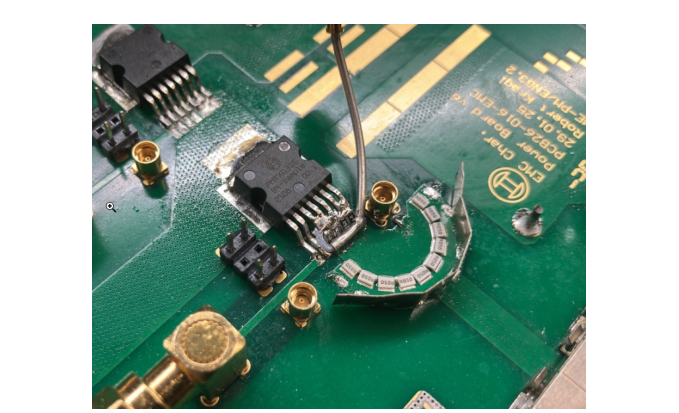
\includegraphics[scale=1]{figures/5_CurrentProbe/Diss_Pic_PShunt.pdf}
	\caption{Realization of the passive shunt for verification.}\label{fig:Diss_Pic_PShunt}
\end{figure}

As a reference, a high-ohmic shunt with \SI{250}{m\Omega} is used.
Its transfer function is shown in \fref{fig:VNA_PShunt}, where it exhibits a \mi{f}{3dB} bandwidth of \SI{385}{MHz}, which is sufficient for the low-pass verification.
The shunts are placed in the commutation loop by replacing the D2PAK source connectors with SMD shunts, while a semi-rigid coaxial SMA cable is used as the pick-up.
A photograph of the setup is shown in \fref{fig:Diss_Pic_PShunt}.

\begin{figure}[ht]
	\centering
	% This file was created by matlab2tikz.
%
%The latest updates can be retrieved from
%  http://www.mathworks.com/matlabcentral/fileexchange/22022-matlab2tikz-matlab2tikz
%where you can also make suggestions and rate matlab2tikz.
%
\definecolor{mycolor1}{rgb}{0.00000,0.44700,0.74100}%
\definecolor{mycolor2}{rgb}{0.85000,0.32500,0.09800}%
\definecolor{mycolor3}{rgb}{0.92900,0.69400,0.12500}%
\definecolor{mycolor4}{rgb}{0.49400,0.18400,0.55600}%
%
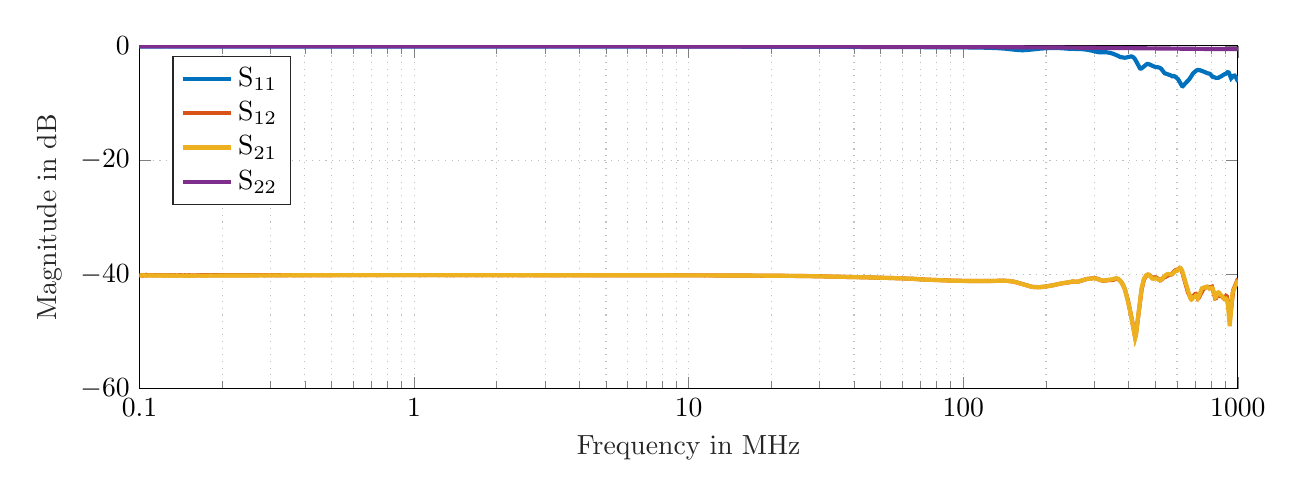
\begin{tikzpicture}

\begin{axis}[%
width=5.492in,
height=1.714in,
at={(0.921in,0.471in)},
scale only axis,
xmode=log,
xmin=0.1,
xmax=1000,
xtick={0.1,1,10,100,1000},
xticklabels={{0.1},{1},{10},{100},{1000}},
xminorticks=true,
xlabel style={font=\color{white!15!black}},
xlabel={Frequency in MHz},
ymin=-60,
ymax=0,
ylabel style={font=\color{white!15!black}},
ylabel={Magnitude in dB},
axis background/.style={fill=white},
xmajorgrids,
xminorgrids,
ymajorgrids,
grid style={dotted},
legend style={at={(0.03,0.97)}, anchor=north west, legend cell align=left, align=left, draw=white!15!black}
]
\addplot [color=mycolor1, line width=1.5pt]
  table[row sep=crcr]{%
0.1	-0.1113608229\\
0.102821974	-0.1106112179\\
0.109876909	-0.1104688438\\
0.111287897	-0.1092707728\\
0.112698884	-0.1118234825\\
0.114815364	-0.1118454559\\
0.117637338	-0.1124389545\\
0.125397767	-0.1073454512\\
0.126808754	-0.1134031677\\
0.128925235	-0.114570386\\
0.130336222	-0.1145717385\\
0.131041715	-0.1103384526\\
0.132452703	-0.1119779867\\
0.138482796	-0.1114999755\\
0.142375573	-0.1102876721\\
0.143348768	-0.112344566\\
0.144321962	-0.110082882\\
0.145295157	-0.1126451274\\
0.146268351	-0.1110470238\\
0.147241545	-0.1135906119\\
0.152107517	-0.1083605748\\
0.154053906	-0.1124386366\\
0.156000295	-0.1105633597\\
0.158919878	-0.1130287254\\
0.167678628	-0.1154593545\\
0.1725446	-0.1146949355\\
0.179356961	-0.11337945\\
0.18811571	-0.111770622\\
0.195596933	-0.1128805991\\
0.198281036	-0.1124944441\\
0.20230719	-0.1125386596\\
0.207675395	-0.1123839266\\
0.21170155	-0.1126398418\\
0.215727704	-0.113347872\\
0.218411806	-0.1115071881\\
0.221095909	-0.1125328129\\
0.242568731	-0.1133762668\\
0.245252834	-0.1155449368\\
0.253305142	-0.1144119577\\
0.260015399	-0.1149780243\\
0.261582765	-0.1129011215\\
0.265273664	-0.1149001057\\
0.268964563	-0.1140331048\\
0.283728159	-0.1145967987\\
0.285573608	-0.1159191863\\
0.289264507	-0.114789227\\
0.318791699	-0.1140271804\\
0.333555295	-0.1151040883\\
0.359701417	-0.1156497128\\
0.367338544	-0.1165967884\\
0.423344138	-0.1166936061\\
0.46152977	-0.1174553846\\
0.476804023	-0.1153271704\\
0.50111614	-0.1162749421\\
0.515158441	-0.1158437643\\
0.543243041	-0.1160138497\\
0.680155469	-0.1207899825\\
0.737524793	-0.1211927714\\
0.77142348	-0.1202581289\\
0.800479497	-0.1216259102\\
0.8634342	-0.1198948633\\
0.887647548	-0.1210627327\\
0.911860895	-0.1196112785\\
0.936074243	-0.1197332703\\
1.02004808	-0.1201004979\\
1.080151181	-0.1203331034\\
1.160288649	-0.1208881514\\
4.814599836	-0.130119183\\
5.079689667	-0.1311582886\\
5.245370812	-0.1305734169\\
5.709278018	-0.1320343714\\
12.12137946	-0.1441270454\\
12.75590504	-0.1462376729\\
14.14671793	-0.1483232934\\
16.58064048	-0.1535159975\\
18.61637613	-0.1571655397\\
19.81168941	-0.1595415421\\
26.59592024	-0.1719262518\\
29.56389918	-0.1775663608\\
33.59463202	-0.1840695569\\
38.14229053	-0.1895243698\\
41.09826856	-0.1932150493\\
47.75921134	-0.203798167\\
50.57327152	-0.207448246\\
56.51406525	-0.2172619196\\
62.66925782	-0.2262863922\\
68.27638994	-0.2352262063\\
86.68817822	-0.2527897827\\
95.61009637	-0.2647249861\\
101.5580418	-0.2754483241\\
110.4799599	-0.2970358458\\
116.7508695	-0.3166355959\\
122.4761667	-0.3423260435\\
132.2909619	-0.4002972338\\
136.38046	-0.4357698632\\
142.1057572	-0.5028596608\\
150.2847533	-0.6260888354\\
156.8279501	-0.7210592943\\
161.675471	-0.7617759064\\
163.9319773	-0.7709072932\\
166.1884837	-0.7658660937\\
169.5732432	-0.7424011749\\
174.0862559	-0.6937666048\\
192.1383066	-0.4829374434\\
198.9078257	-0.4321562403\\
204.5490915	-0.4059328285\\
214.7033701	-0.379972554\\
218.0881296	-0.3814787983\\
222.0936934	-0.3929585063\\
228.3172134	-0.4293759556\\
243.8760136	-0.523343137\\
248.5436536	-0.5208934736\\
251.6554136	-0.5353679438\\
257.8789337	-0.5645015748\\
262.5465737	-0.5733028428\\
267.2142137	-0.5796054784\\
271.8818538	-0.5928294723\\
274.9936138	-0.613489303\\
281.2171338	-0.6809797043\\
292.1082939	-0.8182771563\\
311.8457146	-1.128817165\\
313.9919762	-1.135517682\\
322.5770228	-1.121505785\\
326.8695461	-1.117490279\\
329.0158078	-1.116541881\\
333.3083311	-1.142338545\\
341.8933777	-1.230529947\\
350.4784243	-1.372425101\\
361.2097326	-1.638705342\\
374.0873025	-1.974809758\\
386.9648724	-2.085087879\\
391.2573957	-2.060538843\\
408.4274889	-1.850539442\\
412.7200122	-1.907712784\\
417.0125355	-2.042918132\\
422.486007	-2.373433983\\
440.2443915	-3.956235791\\
443.2041222	-3.989162242\\
446.163853	-3.936744867\\
466.8819682	-3.180001567\\
469.8416989	-3.18358961\\
472.8014297	-3.201017305\\
478.7208912	-3.302849188\\
496.4792757	-3.646659035\\
505.3584679	-3.731002172\\
508.3181987	-3.738016348\\
514.2376601	-3.779659596\\
520.1571216	-3.859616102\\
526.0765831	-4.039125635\\
540.8752369	-4.789228903\\
570.4725443	-5.187640222\\
576.8889099	-5.344268991\\
580.9588239	-5.336143583\\
585.0287378	-5.296303628\\
589.0986518	-5.349723605\\
605.3783076	-5.827910662\\
625.7278773	-7.021709883\\
629.7977913	-7.06793681\\
666.4270168	-5.810631166\\
686.7765866	-4.82529612\\
707.1261563	-4.303448055\\
715.2659843	-4.225291435\\
723.4058122	-4.270881908\\
727.4757261	-4.263196369\\
755.9651238	-4.574391304\\
776.3146935	-4.812197538\\
780.3846075	-4.820948941\\
788.5244354	-4.880846767\\
793.2776401	-4.961608469\\
810.1203919	-5.45482128\\
815.7346424	-5.447785864\\
832.5773941	-5.619102264\\
838.1916447	-5.613850482\\
849.4201459	-5.593566841\\
860.648647	-5.426262612\\
866.2628976	-5.39840847\\
888.7198998	-5.039172915\\
905.5626516	-4.855677208\\
916.7911527	-4.623239343\\
922.4054033	-4.637015036\\
928.0196538	-4.743127492\\
944.8624056	-5.685517709\\
961.7051573	-5.260965507\\
972.9336584	-5.212971692\\
984.1621596	-5.517507873\\
1001.004911	-6.276826078\\
};
\addlegendentry{$\mathrm{S}_\mathrm{11}$}

\addplot [color=mycolor2, line width=1.5pt]
  table[row sep=crcr]{%
0.1	-40.17843466\\
0.101410987	-40.14957287\\
0.102116481	-40.13714666\\
0.102821974	-40.22248108\\
0.103527468	-40.14279048\\
0.104232961	-40.15306646\\
0.104938455	-40.14422265\\
0.105643948	-40.10379595\\
0.106349442	-40.18747815\\
0.107054935	-40.1370117\\
0.107760429	-40.15068797\\
0.109171416	-40.1502343\\
0.109876909	-40.14101046\\
0.110582403	-40.14402163\\
0.111287897	-40.16953993\\
0.11199339	-40.1655318\\
0.112698884	-40.17225231\\
0.113404377	-40.17003459\\
0.115520858	-40.14557651\\
0.116226351	-40.18513349\\
0.117637338	-40.14575152\\
0.118342832	-40.14096041\\
0.119753819	-40.17472517\\
0.120459312	-40.17316128\\
0.121164806	-40.15725303\\
0.1218703	-40.18803398\\
0.122575793	-40.18123489\\
0.123281287	-40.16104951\\
0.124692274	-40.18311073\\
0.126103261	-40.17062657\\
0.126808754	-40.18547802\\
0.127514248	-40.15301345\\
0.128219741	-40.18077612\\
0.128925235	-40.17029635\\
0.129630728	-40.17496507\\
0.131747209	-40.15681052\\
0.132452703	-40.17510491\\
0.133158196	-40.17217735\\
0.13386369	-40.19778307\\
0.135274677	-40.16415689\\
0.136685664	-40.17587112\\
0.137509601	-40.17216422\\
0.138482796	-40.17865891\\
0.13945599	-40.16226761\\
0.140429185	-40.16808386\\
0.141402379	-40.18258126\\
0.142375573	-40.15788797\\
0.144321962	-40.18189224\\
0.145295157	-40.18178542\\
0.146268351	-40.15936497\\
0.14821474	-40.19289413\\
0.150161129	-40.17303273\\
0.152107517	-40.15180526\\
0.153080712	-40.17792863\\
0.154053906	-40.17574153\\
0.155027101	-40.18501332\\
0.156000295	-40.16920778\\
0.156973489	-40.18123101\\
0.158919878	-40.17687991\\
0.159893073	-40.19364933\\
0.160866267	-40.17860451\\
0.161839461	-40.18029065\\
0.162812656	-40.1517051\\
0.16378585	-40.17813492\\
0.165732239	-40.17127354\\
0.166705433	-40.1442627\\
0.167678628	-40.1475192\\
0.169625017	-40.17777611\\
0.171571405	-40.15400439\\
0.174490989	-40.17200655\\
0.175464183	-40.15945531\\
0.176437377	-40.17055246\\
0.177410572	-40.14715946\\
0.178383766	-40.15935314\\
0.179356961	-40.15165001\\
0.180330155	-40.16128972\\
0.181303349	-40.14542968\\
0.182276544	-40.17448969\\
0.183249738	-40.16305179\\
0.184222933	-40.17107023\\
0.186169321	-40.14163719\\
0.187142516	-40.16309846\\
0.18811571	-40.15165667\\
0.189088905	-40.16575151\\
0.190228728	-40.16040135\\
0.191570779	-40.14367621\\
0.19291283	-40.15951388\\
0.194254882	-40.15091171\\
0.199623087	-40.16065009\\
0.200965139	-40.16110234\\
0.20230719	-40.15823493\\
0.203649241	-40.14321912\\
0.204991293	-40.16340251\\
0.207675395	-40.1456019\\
0.209017447	-40.14763968\\
0.210359498	-40.16220311\\
0.21170155	-40.15045109\\
0.213043601	-40.16060264\\
0.214385652	-40.14885493\\
0.217069755	-40.16150555\\
0.221095909	-40.16094809\\
0.22243796	-40.15095312\\
0.225122063	-40.16514013\\
0.226464115	-40.17063416\\
0.229148217	-40.15422715\\
0.23183232	-40.16032832\\
0.234516423	-40.1456574\\
0.237200526	-40.17340574\\
0.24122668	-40.14939796\\
0.242568731	-40.1572823\\
0.243910782	-40.15450757\\
0.245252834	-40.16344976\\
0.249278988	-40.14784334\\
0.250621039	-40.14576938\\
0.251963091	-40.12887113\\
0.254647193	-40.16767606\\
0.258673347	-40.1339611\\
0.261582765	-40.16112109\\
0.263428214	-40.14891417\\
0.265273664	-40.15601156\\
0.267119113	-40.15055255\\
0.268964563	-40.13050742\\
0.270810012	-40.15219958\\
0.272655462	-40.13680739\\
0.274500911	-40.14661191\\
0.276346361	-40.13045696\\
0.27819181	-40.14004455\\
0.28003726	-40.13715656\\
0.281882709	-40.16064844\\
0.283728159	-40.14700234\\
0.287419058	-40.15150007\\
0.289264507	-40.14647533\\
0.291109957	-40.13166396\\
0.292955406	-40.15726136\\
0.296646305	-40.13931818\\
0.300337204	-40.15338688\\
0.302182654	-40.1499421\\
0.305873553	-40.13724783\\
0.309564452	-40.14987553\\
0.311409901	-40.14258872\\
0.313255351	-40.15068924\\
0.3151008	-40.14395866\\
0.31694625	-40.15495608\\
0.318791699	-40.14732838\\
0.320637149	-40.15435856\\
0.322482598	-40.14861012\\
0.324328048	-40.15119173\\
0.326173497	-40.1464815\\
0.328018947	-40.16231289\\
0.329864396	-40.14083471\\
0.331709845	-40.15261665\\
0.333555295	-40.14874531\\
0.335400744	-40.13916564\\
0.337246194	-40.14384606\\
0.339091643	-40.16985954\\
0.340937093	-40.13752884\\
0.342782542	-40.15588303\\
0.344627992	-40.14874324\\
0.346473441	-40.15782781\\
0.348318891	-40.13532368\\
0.35016434	-40.14277512\\
0.353855239	-40.13734202\\
0.355700689	-40.14375773\\
0.359701417	-40.14239863\\
0.362247126	-40.14973772\\
0.364792835	-40.14440907\\
0.367338544	-40.14683935\\
0.369884252	-40.15999144\\
0.372429961	-40.13180933\\
0.377521379	-40.15734371\\
0.380067088	-40.13624115\\
0.382612797	-40.15053054\\
0.385158505	-40.14511749\\
0.387704214	-40.12908107\\
0.390249923	-40.15540276\\
0.392795632	-40.14594501\\
0.395341341	-40.15034826\\
0.400432758	-40.13664645\\
0.402978467	-40.14719659\\
0.410615594	-40.13792604\\
0.415707011	-40.15554418\\
0.41825272	-40.13903466\\
0.420798429	-40.15676544\\
0.425889847	-40.14065799\\
0.428435555	-40.14422745\\
0.430981264	-40.13681132\\
0.433526973	-40.14401185\\
0.436072682	-40.13862777\\
0.438618391	-40.14034256\\
0.441164099	-40.13222539\\
0.443709808	-40.15895914\\
0.446255517	-40.13295404\\
0.453892644	-40.15198747\\
0.458984061	-40.12737167\\
0.46152977	-40.14361297\\
0.466621188	-40.14922811\\
0.471712605	-40.14246887\\
0.474258314	-40.14593654\\
0.476804023	-40.13601637\\
0.479349732	-40.13977015\\
0.481895441	-40.15419417\\
0.486986858	-40.13261781\\
0.489532567	-40.15313514\\
0.494623985	-40.12530015\\
0.497605565	-40.15782102\\
0.504626715	-40.13823081\\
0.50813729	-40.14261048\\
0.511647866	-40.14177292\\
0.515158441	-40.12904695\\
0.522179591	-40.13797929\\
0.529200741	-40.13696927\\
0.532711316	-40.14661065\\
0.539732466	-40.12918164\\
0.543243041	-40.12794969\\
0.546753616	-40.13443902\\
0.550264191	-40.12918301\\
0.553774767	-40.14596587\\
0.560795917	-40.13493316\\
0.571327642	-40.14898159\\
0.574838217	-40.12851777\\
0.581859367	-40.14506035\\
0.585369942	-40.1474262\\
0.592391092	-40.13277727\\
0.595901667	-40.11953145\\
0.606433393	-40.14438645\\
0.609943968	-40.13567975\\
0.613454543	-40.13741508\\
0.620475693	-40.13269724\\
0.627496843	-40.14106971\\
0.634517993	-40.14683772\\
0.645049719	-40.14168808\\
0.648560294	-40.13338123\\
0.652070869	-40.14428936\\
0.659092019	-40.1379138\\
0.666113169	-40.14650535\\
0.673134319	-40.13538915\\
0.676644894	-40.14322544\\
0.680155469	-40.12717892\\
0.689098098	-40.14199552\\
0.713311446	-40.14299027\\
0.722996785	-40.13073335\\
0.732682124	-40.15412948\\
0.737524793	-40.13598557\\
0.747210132	-40.1479754\\
0.756895471	-40.1338972\\
0.761738141	-40.1424693\\
0.76658081	-40.13732338\\
0.776266149	-40.14519224\\
0.781108819	-40.12932424\\
0.790794158	-40.13711161\\
0.795636827	-40.13969529\\
0.800479497	-40.13257054\\
0.805322166	-40.13471515\\
0.810164836	-40.14141339\\
0.834378183	-40.13330576\\
0.839220853	-40.14754905\\
0.844063522	-40.14550851\\
0.848906192	-40.13593666\\
0.8634342	-40.1416045\\
0.86827687	-40.13835704\\
0.877962209	-40.14519658\\
0.882804878	-40.13575059\\
0.887647548	-40.14324468\\
0.907018226	-40.13699416\\
0.911860895	-40.14673792\\
0.916703565	-40.12928007\\
0.926388904	-40.13928538\\
0.936074243	-40.13534353\\
0.940916912	-40.14003267\\
0.953266857	-40.13116876\\
0.966623102	-40.13526694\\
0.973301224	-40.13614093\\
0.986657469	-40.1421288\\
0.993335591	-40.12917864\\
1.000013714	-40.13262544\\
1.006691836	-40.14546394\\
1.02004808	-40.13659603\\
1.026726203	-40.14163691\\
1.033404325	-40.13480473\\
1.04676057	-40.15394272\\
1.066794937	-40.13297697\\
1.080151181	-40.13794273\\
1.086829304	-40.14141529\\
1.093507426	-40.13845034\\
1.100185548	-40.1499027\\
1.10686367	-40.14212965\\
1.120219915	-40.13550195\\
1.126898037	-40.14396673\\
1.13357616	-40.14145247\\
1.140254282	-40.13214723\\
1.146932404	-40.13418595\\
1.153610527	-40.14472524\\
1.160288649	-40.14171553\\
1.173644894	-40.14254996\\
1.187001138	-40.135496\\
1.200357383	-40.14322181\\
1.213713627	-40.13380476\\
1.22039175	-40.14375821\\
1.227069872	-40.13351746\\
1.233747994	-40.1472008\\
1.247104239	-40.13919785\\
1.260460484	-40.13302511\\
1.267138606	-40.13867008\\
1.273816728	-40.13277398\\
1.287172973	-40.14423268\\
1.293851095	-40.13358841\\
1.320016515	-40.15144249\\
1.338382633	-40.13011476\\
1.356748752	-40.14918631\\
1.375114871	-40.14215994\\
1.38429793	-40.14571218\\
1.393480989	-40.14451906\\
1.402664049	-40.14936\\
1.430213227	-40.12811029\\
1.439396286	-40.14125971\\
1.448579346	-40.12957017\\
1.466945464	-40.14929669\\
1.476128524	-40.13528378\\
1.494494642	-40.14553108\\
1.512860761	-40.13424564\\
1.53122688	-40.14096981\\
1.540409939	-40.1576145\\
1.549592999	-40.1343654\\
1.558776058	-40.14891792\\
1.567959117	-40.14320462\\
1.577142177	-40.14700957\\
1.595508295	-40.13007331\\
1.613874414	-40.13379059\\
1.623057473	-40.14474998\\
1.650606652	-40.13374234\\
1.66897277	-40.14228776\\
1.67815583	-40.14030352\\
1.687338889	-40.13141762\\
1.696521948	-40.14997278\\
1.705705008	-40.14140467\\
1.714888067	-40.14885205\\
1.724071126	-40.13769687\\
1.742437245	-40.14013107\\
1.760803364	-40.13828013\\
1.769986423	-40.15203211\\
1.802561859	-40.13644513\\
1.815229447	-40.14547547\\
1.827897036	-40.13485998\\
1.840564625	-40.13922492\\
1.853232214	-40.13591773\\
1.878567391	-40.14342156\\
1.89123498	-40.13398714\\
1.929237746	-40.14593271\\
1.941905335	-40.15086669\\
1.954572924	-40.13155099\\
1.967240513	-40.1426846\\
1.979908101	-40.12942276\\
1.99257569	-40.14045709\\
2.005243279	-40.1375586\\
2.017910868	-40.14715\\
2.030578457	-40.14485921\\
2.043246045	-40.15227488\\
2.068581223	-40.14293377\\
2.0939164	-40.15046118\\
2.131919167	-40.13486273\\
2.144586756	-40.14290948\\
2.169921933	-40.13894979\\
2.195257111	-40.14963087\\
2.207924699	-40.14784983\\
2.220592288	-40.13570547\\
2.245927466	-40.14219471\\
2.271262643	-40.13545009\\
2.283930232	-40.15055046\\
2.296597821	-40.13610529\\
2.30926541	-40.1463923\\
2.321932998	-40.13431713\\
2.334600587	-40.14078034\\
2.347268176	-40.13075144\\
2.359935765	-40.13577249\\
2.372603353	-40.15093661\\
2.385270942	-40.14313228\\
2.41060612	-40.14668664\\
2.423273708	-40.14004418\\
2.435941297	-40.156252\\
2.448608886	-40.14134383\\
2.493581802	-40.15186345\\
2.511050619	-40.14703864\\
2.528519436	-40.15189967\\
2.545988253	-40.14028699\\
2.580925887	-40.14591818\\
2.615863521	-40.14051714\\
2.650801155	-40.15020864\\
2.668269972	-40.13638634\\
2.685738789	-40.1439577\\
2.703207606	-40.13370542\\
2.73814524	-40.15926837\\
2.755614057	-40.14384303\\
2.790551691	-40.15081659\\
2.808020508	-40.14600869\\
2.842958142	-40.15233987\\
2.860426959	-40.14430382\\
2.877895776	-40.14556942\\
2.895364593	-40.15498514\\
2.91283341	-40.13737397\\
2.947771044	-40.15860274\\
2.965239861	-40.14236781\\
2.982708678	-40.15614658\\
3.000177495	-40.12955561\\
3.035115129	-40.15750087\\
3.087521579	-40.14663503\\
3.104990396	-40.15793297\\
3.122459213	-40.1471738\\
3.13992803	-40.15918717\\
3.157396847	-40.1401604\\
3.174865664	-40.15451208\\
3.244740932	-40.14184076\\
3.262209749	-40.15235347\\
3.297147383	-40.1417768\\
3.3146162	-40.15356658\\
3.332085017	-40.14067169\\
3.367022651	-40.15319027\\
3.384491468	-40.15078415\\
3.404893095	-40.13987783\\
3.428914395	-40.1489241\\
3.452935696	-40.14444239\\
3.476956996	-40.13379164\\
3.500978297	-40.15498443\\
3.524999597	-40.15388628\\
3.549020898	-40.14889292\\
3.573042199	-40.15208513\\
3.6210848	-40.13251199\\
3.669127401	-40.14986323\\
3.717170002	-40.13760733\\
3.765212603	-40.15376216\\
3.813255204	-40.14743009\\
3.861297806	-40.15088328\\
3.885319106	-40.1540356\\
3.933361707	-40.15042243\\
3.957383008	-40.15601466\\
4.005425609	-40.14078405\\
4.02944691	-40.16164067\\
4.05346821	-40.15116487\\
4.101510811	-40.15854006\\
4.125532112	-40.14642237\\
4.149553413	-40.1494155\\
4.197596014	-40.14046566\\
4.245638615	-40.1581879\\
4.293681216	-40.14553371\\
4.317702517	-40.1564265\\
4.341723817	-40.14344683\\
4.365745118	-40.14627291\\
4.389766418	-40.14424329\\
4.413787719	-40.15280532\\
4.43780902	-40.1414939\\
4.46183032	-40.14778967\\
4.485851621	-40.14602508\\
4.509872921	-40.15668245\\
4.533894222	-40.14671412\\
4.557915522	-40.15104252\\
4.581936823	-40.14584197\\
4.605958124	-40.15642747\\
4.629979424	-40.14645071\\
4.68205492	-40.15452002\\
4.715191149	-40.1445494\\
4.748327378	-40.16053152\\
4.847736065	-40.14118462\\
4.880872294	-40.16065897\\
4.914008523	-40.1490109\\
4.947144752	-40.15312512\\
4.980280981	-40.14821897\\
5.01341721	-40.15847643\\
5.046553439	-40.15433609\\
5.112825896	-40.15677557\\
5.145962125	-40.14177745\\
5.245370812	-40.15437959\\
5.278507041	-40.14619728\\
5.344779499	-40.16480866\\
5.377915728	-40.15111568\\
5.411051957	-40.15531901\\
5.444188186	-40.15000805\\
5.477324415	-40.15796152\\
5.543596873	-40.14671406\\
5.576733102	-40.16406199\\
5.609869331	-40.13668899\\
5.676141789	-40.15916853\\
5.742414247	-40.15845718\\
5.808686704	-40.1515013\\
5.908095391	-40.16077067\\
5.94123162	-40.15524218\\
6.007504078	-40.16205853\\
6.073776536	-40.16830308\\
6.106912765	-40.15941874\\
6.140048994	-40.16221046\\
6.173185223	-40.15480805\\
6.206321452	-40.15941911\\
6.239457681	-40.15476875\\
6.305730139	-40.16348658\\
6.372002597	-40.15234039\\
6.405138826	-40.15855367\\
6.438275055	-40.15562287\\
6.477084809	-40.16200105\\
6.522780223	-40.15081337\\
6.568475638	-40.16409115\\
6.659866467	-40.15438698\\
6.79695271	-40.16279693\\
6.842648125	-40.15173792\\
6.934038953	-40.16222536\\
6.979734368	-40.15571073\\
7.071125197	-40.16647139\\
7.116820611	-40.16832935\\
7.162516026	-40.15862968\\
7.20821144	-40.16254289\\
7.253906855	-40.15295858\\
7.299602269	-40.1690639\\
7.345297683	-40.16161292\\
7.390993098	-40.16774994\\
7.482383927	-40.156209\\
7.573774756	-40.16678998\\
7.665165585	-40.16987293\\
7.756556413	-40.16382674\\
7.847947242	-40.16861796\\
7.939338071	-40.1602427\\
7.985033486	-40.16512731\\
8.0307289	-40.16155987\\
8.122119729	-40.17176571\\
8.167815143	-40.15340436\\
8.259205972	-40.16905137\\
8.350596801	-40.1668791\\
8.396292216	-40.16101017\\
8.44198763	-40.16822693\\
8.533378459	-40.16796554\\
8.579073873	-40.179606\\
8.670464702	-40.16638524\\
8.716160117	-40.177836\\
8.761855531	-40.16535048\\
8.85324636	-40.17378595\\
8.906613499	-40.16693901\\
8.969648125	-40.17699592\\
9.095717379	-40.16512926\\
9.158752005	-40.17769726\\
9.221786632	-40.17214227\\
9.284821259	-40.17670483\\
9.347855886	-40.17580911\\
9.410890512	-40.18012816\\
9.536959766	-40.16851819\\
9.599994392	-40.17405765\\
9.726063646	-40.17077009\\
9.789098272	-40.17547606\\
9.915167526	-40.17054306\\
10.04123678	-40.17499611\\
10.10427141	-40.17154604\\
10.23034066	-40.18245159\\
10.29337529	-40.1711278\\
10.35640991	-40.18488818\\
10.48247917	-40.17324475\\
10.54551379	-40.18052928\\
10.67158305	-40.172992\\
10.7976523	-40.18329759\\
10.86068693	-40.1786333\\
10.92372155	-40.18603431\\
11.11282543	-40.17458381\\
11.17586006	-40.18637676\\
11.30192931	-40.17598351\\
11.42799857	-40.19360328\\
11.49103319	-40.1782822\\
11.55406782	-40.18687528\\
11.68013707	-40.18132102\\
11.7431717	-40.18616151\\
11.80620633	-40.18393473\\
11.86924095	-40.17470862\\
11.93227558	-40.18808874\\
11.99531021	-40.17760228\\
12.05834483	-40.18709488\\
12.12137946	-40.18143716\\
12.18441409	-40.19552706\\
12.24744871	-40.17736384\\
12.58205343	-40.20089465\\
12.75590504	-40.19142956\\
12.84283085	-40.18287668\\
12.92975665	-40.19886166\\
13.01668246	-40.18580722\\
13.19053407	-40.19299628\\
13.36438568	-40.1920896\\
13.45131149	-40.18925451\\
13.53823729	-40.19937691\\
13.6251631	-40.19502977\\
13.7120889	-40.21501113\\
13.79901471	-40.19683017\\
13.88594051	-40.19967439\\
13.97286632	-40.19474704\\
14.05979212	-40.19590902\\
14.14671793	-40.19211689\\
14.40749535	-40.20828763\\
14.49442115	-40.19608312\\
14.58134696	-40.20208637\\
14.75519857	-40.19486283\\
14.92905018	-40.20518818\\
15.01597598	-40.18914217\\
15.1898276	-40.21477782\\
15.2767534	-40.20662558\\
15.36367921	-40.21032474\\
15.53753082	-40.20166742\\
15.79830823	-40.2068265\\
15.88523404	-40.20101747\\
16.05908565	-40.21321663\\
16.23293726	-40.2054316\\
16.40678887	-40.20869168\\
16.58064048	-40.21232271\\
16.66756629	-40.2181736\\
16.94293753	-40.21187053\\
17.30153151	-40.22099137\\
17.42106284	-40.23056994\\
17.54059417	-40.21401272\\
17.77965683	-40.22108143\\
17.89918816	-40.22835821\\
18.13825081	-40.22237159\\
18.25778214	-40.23526702\\
18.37731347	-40.23330247\\
18.4968448	-40.22573626\\
18.61637613	-40.23659133\\
18.73590746	-40.22269906\\
19.3335641	-40.23835535\\
19.45309543	-40.23128728\\
19.69215808	-40.23711652\\
19.81168941	-40.24142841\\
19.93122074	-40.23257224\\
20.05075207	-40.24200084\\
20.28981473	-40.23191863\\
20.40934606	-40.24833572\\
20.76794004	-40.23606112\\
21.0070027	-40.24885596\\
21.24606536	-40.25459983\\
21.36559668	-40.2374774\\
21.48512801	-40.25573046\\
21.60465934	-40.2490771\\
21.72419067	-40.25654783\\
21.843722	-40.24537443\\
21.96325333	-40.26721783\\
22.08278466	-40.25391816\\
22.20231598	-40.26380794\\
22.32184731	-40.25553923\\
22.6804413	-40.26944104\\
22.91950396	-40.25676249\\
23.03903528	-40.26734036\\
23.15856661	-40.26293447\\
23.29816585	-40.27084251\\
23.46305357	-40.26207982\\
23.62794129	-40.27554652\\
23.79282901	-40.27599438\\
23.95771673	-40.26324617\\
24.12260444	-40.27040291\\
24.28749217	-40.26900439\\
24.45237988	-40.27219033\\
24.78215532	-40.28901239\\
24.94704304	-40.27956766\\
25.11193076	-40.28289428\\
25.27681848	-40.28064952\\
25.60659392	-40.29310416\\
26.10125708	-40.30112025\\
26.43103252	-40.30680757\\
26.59592024	-40.29178797\\
26.76080796	-40.29844128\\
26.92569568	-40.28749949\\
27.09058339	-40.31267125\\
27.25547111	-40.30065587\\
27.42035883	-40.31231848\\
27.75013427	-40.31132816\\
27.91502199	-40.32020556\\
28.07990971	-40.3082569\\
28.24479743	-40.31181682\\
28.57457287	-40.33202174\\
28.73946059	-40.3211275\\
28.90434831	-40.32294768\\
29.23412375	-40.33556738\\
29.39901147	-40.33253328\\
29.56389919	-40.33480149\\
29.7287869	-40.32372883\\
29.89367462	-40.34447868\\
30.05856234	-40.33914993\\
30.38833778	-40.34711544\\
30.5532255	-40.34469561\\
31.3776641	-40.3686096\\
31.54255182	-40.36329895\\
31.70743954	-40.36525411\\
32.23033447	-40.39357417\\
32.4577174	-40.38673197\\
32.68510032	-40.39571041\\
32.91248325	-40.38533803\\
33.13986618	-40.39549652\\
33.3672491	-40.39037276\\
33.59463203	-40.40548527\\
33.82201495	-40.40228895\\
34.04939788	-40.41657615\\
34.2767808	-40.40680325\\
34.50416373	-40.41101625\\
34.73154665	-40.42553777\\
34.95892958	-40.41784143\\
35.64107835	-40.42288529\\
35.86846128	-40.43726056\\
36.0958442	-40.43321286\\
36.32322713	-40.4391194\\
36.55061005	-40.4317961\\
36.77799298	-40.44100958\\
37.23275883	-40.44098338\\
37.46014176	-40.44785789\\
37.68752468	-40.4659622\\
37.91490761	-40.46362679\\
38.14229053	-40.45607919\\
38.59705638	-40.46456733\\
38.82443931	-40.47522702\\
39.05182223	-40.46712608\\
39.50658808	-40.47160765\\
39.73397101	-40.48705578\\
39.96135393	-40.47326014\\
40.18873686	-40.49093709\\
40.41611979	-40.47690902\\
41.32565149	-40.49862425\\
41.55303441	-40.48981655\\
42.00780026	-40.50266118\\
42.23518319	-40.49443108\\
42.68994904	-40.5034475\\
42.91733196	-40.51902777\\
43.37209781	-40.51334287\\
44.31980444	-40.53470706\\
44.94515115	-40.5252122\\
45.57049786	-40.54413347\\
45.88317121	-40.5371187\\
46.50851792	-40.5506181\\
47.13386463	-40.54847186\\
47.75921134	-40.57178884\\
48.07188469	-40.56117681\\
48.6972314	-40.57524297\\
49.32257811	-40.58669212\\
49.63525146	-40.57231566\\
49.94792482	-40.59446904\\
50.26059817	-40.57434098\\
51.51129158	-40.61365237\\
52.13663829	-40.61021226\\
52.44931165	-40.62350863\\
52.761985	-40.61790524\\
53.38733171	-40.6296376\\
54.01267842	-40.62701687\\
54.32535177	-40.64000082\\
55.26337183	-40.65095656\\
55.57604519	-40.6494252\\
55.88871854	-40.66259702\\
56.2013919	-40.65931491\\
56.51406525	-40.66191863\\
56.82673861	-40.68202811\\
57.45208531	-40.68133658\\
58.07743202	-40.69524675\\
58.39010538	-40.69291683\\
59.32812544	-40.70490077\\
59.95347215	-40.7146508\\
60.2661455	-40.70730953\\
60.9439864	-40.72167459\\
61.80662211	-40.73377858\\
62.23793996	-40.74287039\\
62.66925782	-40.74058914\\
63.10057567	-40.74592127\\
63.53189353	-40.75847241\\
63.96321139	-40.74894343\\
64.82584709	-40.76017211\\
65.25716495	-40.77198029\\
65.68848281	-40.76712357\\
66.55111852	-40.81245671\\
66.98243637	-40.80124322\\
67.84507208	-40.83100654\\
68.27638994	-40.83032189\\
69.13902565	-40.87184873\\
69.5703435	-40.86263553\\
70.00166136	-40.86555698\\
70.43297921	-40.88837561\\
70.86429707	-40.86628603\\
72.15825064	-40.90887389\\
77.3340649	-40.97473243\\
77.76538276	-40.96850745\\
79.05933632	-40.98577858\\
79.49065418	-40.97180734\\
79.92197203	-41.00736428\\
81.2159256	-41.00163548\\
81.64724345	-41.00615232\\
82.07856131	-41.01761866\\
82.94119702	-41.01844037\\
83.80383273	-41.03939352\\
84.9037946	-41.03013433\\
87.28297277	-41.06613007\\
87.87776731	-41.06151425\\
90.85174002	-41.09831952\\
91.44653457	-41.09200704\\
92.04132911	-41.09273818\\
93.2309182	-41.10387741\\
93.82571274	-41.10728987\\
94.42050728	-41.10586121\\
95.01530183	-41.11144175\\
96.20489091	-41.12666053\\
96.79968545	-41.13338015\\
97.39448	-41.1250789\\
98.58406908	-41.13488083\\
99.77365817	-41.15049073\\
100.9632473	-41.13854949\\
102.1528363	-41.15502084\\
102.7476309	-41.14609929\\
103.3424254	-41.14801559\\
103.93722	-41.15762626\\
105.1268091	-41.16023351\\
105.7216036	-41.1672126\\
106.9111927	-41.16085776\\
107.5059872	-41.17031486\\
108.1007818	-41.16378972\\
109.2903709	-41.17219337\\
110.4799599	-41.17782233\\
111.669549	-41.15675768\\
112.2643436	-41.18401478\\
112.8591381	-41.16157756\\
115.2383163	-41.17956604\\
115.9329699	-41.17522241\\
116.7508695	-41.1792926\\
119.2045683	-41.16904669\\
120.0224679	-41.17492014\\
120.8403675	-41.16662921\\
121.6582671	-41.17526607\\
122.4761667	-41.17094629\\
123.2940663	-41.17640724\\
124.9298655	-41.16397894\\
125.7477651	-41.15703924\\
127.3835643	-41.16131294\\
129.0193635	-41.14578278\\
129.8372631	-41.15428631\\
131.4730623	-41.14416635\\
132.290962	-41.14635018\\
133.9267612	-41.12879262\\
134.7446608	-41.13014002\\
135.5625604	-41.12725188\\
136.38046	-41.13108972\\
137.1983596	-41.11042678\\
138.0162592	-41.12501568\\
139.6520584	-41.12136028\\
140.469958	-41.13068057\\
141.2878576	-41.12407143\\
142.9236568	-41.14021492\\
143.7415564	-41.13787172\\
144.559456	-41.15057443\\
145.3773556	-41.1475772\\
151.9205525	-41.26306577\\
155.1921509	-41.36119591\\
159.4189647	-41.52068437\\
166.1884837	-41.7649589\\
177.4710154	-42.17703318\\
178.5992686	-42.18399533\\
180.8557749	-42.21302948\\
181.9840281	-42.21956962\\
183.1122813	-42.23769801\\
184.2405344	-42.21743759\\
187.6252939	-42.24670952\\
188.7535471	-42.23456323\\
189.8818003	-42.23617902\\
194.394813	-42.1900993\\
196.6513193	-42.15328579\\
197.7795725	-42.16123618\\
201.164332	-42.09543531\\
210.1903574	-41.94590144\\
220.5378134	-41.7284831\\
225.2054534	-41.63718466\\
231.4289735	-41.5445264\\
234.5407335	-41.50634864\\
239.2083735	-41.44534162\\
245.4318936	-41.36984215\\
250.0995336	-41.24988305\\
254.7671736	-41.28566505\\
256.3230536	-41.31743734\\
257.8789337	-41.31235371\\
262.5465737	-41.26321935\\
267.2142137	-41.15869127\\
271.8818538	-41.04364474\\
279.6612538	-40.84583379\\
284.3288938	-40.78138117\\
285.8847739	-40.78736478\\
287.4406539	-40.78203848\\
298.3318139	-40.64828683\\
301.443574	-40.67033986\\
303.260668	-40.68311466\\
309.6994529	-40.83481022\\
316.1382379	-41.00776569\\
322.5770228	-41.11869136\\
324.7232845	-41.11470484\\
333.3083311	-41.05634757\\
341.8933777	-41.00087824\\
344.0396394	-41.01407372\\
348.3321627	-40.99176296\\
350.4784243	-40.99374109\\
352.624686	-40.96261922\\
359.0634709	-40.7658257\\
361.2097326	-40.75585988\\
365.5022559	-40.80606058\\
371.9410408	-41.07577032\\
378.3798258	-41.52293796\\
386.9648724	-42.47084289\\
397.6961807	-44.53638649\\
410.5737506	-47.76380911\\
422.486007	-51.01823903\\
425.4457377	-50.50394914\\
446.163853	-42.62334739\\
455.0430452	-40.90444413\\
463.9222374	-40.24315655\\
469.8416989	-40.06027678\\
472.8014297	-40.06903025\\
475.7611604	-40.11378288\\
487.6000834	-40.57540732\\
490.5598142	-40.55547155\\
493.5195449	-40.56391448\\
499.4390064	-40.51404427\\
502.3987372	-40.52563559\\
511.2779294	-40.74626883\\
520.1571216	-41.06791647\\
523.1168524	-41.04899281\\
529.0363139	-40.83735569\\
537.9155061	-40.51651694\\
543.8349676	-40.46698129\\
558.6336214	-40.1461349\\
564.5530828	-40.073152\\
570.4725443	-40.04210466\\
573.4322751	-40.00381612\\
589.0986518	-39.36123671\\
597.2384797	-39.19630681\\
601.3083936	-39.23595794\\
613.5181355	-38.88459677\\
617.5880494	-38.94805481\\
625.7278773	-39.44800879\\
658.2871889	-43.16398096\\
674.5668447	-44.22216111\\
678.6367587	-44.14255759\\
698.9863284	-43.43814253\\
703.0562424	-43.40876399\\
707.1261563	-43.54852956\\
715.2659843	-44.24483693\\
719.3358982	-44.16758254\\
747.8252959	-42.64034106\\
760.0350377	-42.35061993\\
772.2447796	-42.16486545\\
780.3846075	-42.1974402\\
788.5244354	-42.3184397\\
804.5061413	-42.16127474\\
821.348893	-43.68766032\\
826.9631436	-44.21592963\\
832.5773941	-44.17178902\\
843.8058953	-43.52229241\\
849.4201459	-43.50704648\\
855.0343964	-43.57561315\\
860.648647	-43.75381548\\
866.2628976	-43.71405894\\
888.7198998	-44.23104987\\
894.3341504	-44.22801436\\
905.5626516	-43.77258973\\
911.1769021	-43.85194196\\
922.4054033	-45.02700108\\
933.6339044	-48.24328478\\
961.7051573	-42.78237558\\
1001.004911	-40.73237113\\
};
\addlegendentry{$\mathrm{S}_\mathrm{12}$}

\addplot [color=mycolor3, line width=1.5pt]
  table[row sep=crcr]{%
0.1	-40.13672969\\
0.101410987	-40.20213107\\
0.102116481	-40.17188952\\
0.102821974	-40.19882024\\
0.103527468	-40.13244592\\
0.104232961	-40.19822259\\
0.104938455	-40.18028155\\
0.105643948	-40.23235271\\
0.107760429	-40.17477706\\
0.109171416	-40.21216485\\
0.109876909	-40.17114398\\
0.110582403	-40.20567223\\
0.111287897	-40.17576097\\
0.11199339	-40.2342252\\
0.112698884	-40.20170176\\
0.113404377	-40.21482276\\
0.114109871	-40.20911863\\
0.115520858	-40.21576977\\
0.116226351	-40.18819294\\
0.116931845	-40.21182588\\
0.118342832	-40.19108455\\
0.119753819	-40.21585347\\
0.120459312	-40.21130558\\
0.121164806	-40.19443959\\
0.122575793	-40.24488257\\
0.123281287	-40.19708601\\
0.12398678	-40.23400146\\
0.124692274	-40.21222091\\
0.125397767	-40.21890247\\
0.126808754	-40.19573652\\
0.127514248	-40.24397142\\
0.128219741	-40.20706291\\
0.128925235	-40.23798507\\
0.129630728	-40.21679107\\
0.130336222	-40.22848406\\
0.131041715	-40.20222051\\
0.131747209	-40.24079719\\
0.132452703	-40.20679089\\
0.133158196	-40.23251164\\
0.13386369	-40.21805198\\
0.134569183	-40.23124973\\
0.135274677	-40.22520861\\
0.13598017	-40.23213146\\
0.136685664	-40.19644406\\
0.137509601	-40.23547585\\
0.138482796	-40.23282196\\
0.13945599	-40.21948141\\
0.141402379	-40.22443386\\
0.143348768	-40.20718163\\
0.144321962	-40.20815792\\
0.146268351	-40.2471779\\
0.14821474	-40.22931731\\
0.149187934	-40.24728155\\
0.150161129	-40.24389907\\
0.152107517	-40.22810375\\
0.153080712	-40.24265085\\
0.154053906	-40.2105596\\
0.156000295	-40.24357499\\
0.158919878	-40.22605096\\
0.159893073	-40.24329223\\
0.160866267	-40.22298198\\
0.161839461	-40.22758612\\
0.164759045	-40.21378741\\
0.167678628	-40.2455758\\
0.169625017	-40.22551516\\
0.171571405	-40.23843377\\
0.1725446	-40.23344131\\
0.173517794	-40.24039639\\
0.175464183	-40.23068919\\
0.176437377	-40.23997637\\
0.181303349	-40.19921568\\
0.182276544	-40.20844127\\
0.183249738	-40.22932502\\
0.184222933	-40.21304804\\
0.186169321	-40.22296433\\
0.187142516	-40.2156352\\
0.18811571	-40.22660106\\
0.190228728	-40.21591521\\
0.191570779	-40.22008256\\
0.19291283	-40.21746817\\
0.194254882	-40.20575593\\
0.195596933	-40.22461837\\
0.198281036	-40.20468795\\
0.199623087	-40.20441997\\
0.200965139	-40.23373315\\
0.203649241	-40.19612168\\
0.204991293	-40.22660542\\
0.206333344	-40.22043692\\
0.207675395	-40.20165006\\
0.210359498	-40.20910208\\
0.21170155	-40.22165292\\
0.213043601	-40.19723285\\
0.214385652	-40.20587697\\
0.217069755	-40.19269577\\
0.219753858	-40.22224101\\
0.22243796	-40.19616235\\
0.223780012	-40.20780728\\
0.225122063	-40.20647518\\
0.226464115	-40.1992429\\
0.227806166	-40.20910438\\
0.230490269	-40.1993074\\
0.23183232	-40.20452063\\
0.234516423	-40.19501076\\
0.237200526	-40.20107651\\
0.238542577	-40.19509163\\
0.239884628	-40.21238379\\
0.24122668	-40.18251988\\
0.242568731	-40.20569443\\
0.245252834	-40.18421039\\
0.247936937	-40.20774223\\
0.250621039	-40.18655754\\
0.253305142	-40.2058331\\
0.258673347	-40.18542898\\
0.261582765	-40.19405621\\
0.263428214	-40.19182623\\
0.265273664	-40.20113923\\
0.267119113	-40.18731631\\
0.270810012	-40.1938919\\
0.272655462	-40.18511438\\
0.274500911	-40.18691431\\
0.27819181	-40.18265166\\
0.28003726	-40.17429996\\
0.281882709	-40.17858495\\
0.283728159	-40.1746379\\
0.285573608	-40.20223635\\
0.287419058	-40.18590518\\
0.289264507	-40.18679432\\
0.291109957	-40.18160247\\
0.292955406	-40.19150448\\
0.296646305	-40.16126143\\
0.300337204	-40.1858435\\
0.302182654	-40.17918145\\
0.304028103	-40.19472926\\
0.307719002	-40.17437069\\
0.309564452	-40.17012116\\
0.311409901	-40.17869792\\
0.3151008	-40.1712331\\
0.31694625	-40.18830405\\
0.318791699	-40.17393106\\
0.320637149	-40.18334779\\
0.322482598	-40.17479749\\
0.324328048	-40.18231118\\
0.326173497	-40.17286077\\
0.328018947	-40.17871318\\
0.331709845	-40.16155985\\
0.333555295	-40.17677871\\
0.335400744	-40.16000801\\
0.339091643	-40.17800901\\
0.340937093	-40.16820367\\
0.342782542	-40.17984649\\
0.344627992	-40.17007572\\
0.346473441	-40.17324511\\
0.348318891	-40.16304025\\
0.35200979	-40.17729587\\
0.355700689	-40.16588436\\
0.357546138	-40.17468987\\
0.359701417	-40.17243919\\
0.362247126	-40.15183991\\
0.364792835	-40.16681343\\
0.367338544	-40.16264349\\
0.369884252	-40.16842483\\
0.372429961	-40.16404154\\
0.37497567	-40.15418279\\
0.377521379	-40.16772222\\
0.380067088	-40.16084461\\
0.382612797	-40.16621006\\
0.385158505	-40.1580401\\
0.387704214	-40.16960831\\
0.392795632	-40.16361586\\
0.395341341	-40.17038833\\
0.400432758	-40.15689074\\
0.402978467	-40.16397551\\
0.405524176	-40.16221009\\
0.408069885	-40.14095564\\
0.410615594	-40.16214773\\
0.415707011	-40.1530737\\
0.41825272	-40.15162201\\
0.423344138	-40.15500815\\
0.425889847	-40.14368722\\
0.428435555	-40.15125087\\
0.430981264	-40.14626586\\
0.433526973	-40.14815719\\
0.436072682	-40.142507\\
0.438618391	-40.15480536\\
0.441164099	-40.1381386\\
0.443709808	-40.1517365\\
0.448801226	-40.13554811\\
0.451346935	-40.15652354\\
0.453892644	-40.14356169\\
0.458984061	-40.15071019\\
0.466621188	-40.13968234\\
0.471712605	-40.13947866\\
0.476804023	-40.15359049\\
0.479349732	-40.14466985\\
0.481895441	-40.15190603\\
0.486986858	-40.14096369\\
0.489532567	-40.15203201\\
0.492078276	-40.14831648\\
0.497605565	-40.15285286\\
0.50111614	-40.14473659\\
0.518669016	-40.15198932\\
0.522179591	-40.13650384\\
0.525690166	-40.148556\\
0.529200741	-40.1326317\\
0.532711316	-40.16110851\\
0.539732466	-40.14214428\\
0.543243041	-40.14569601\\
0.546753616	-40.12897282\\
0.550264191	-40.14295052\\
0.557285342	-40.13115243\\
0.560795917	-40.13191182\\
0.564306492	-40.14145618\\
0.567817067	-40.13322698\\
0.571327642	-40.14363307\\
0.578348792	-40.13524754\\
0.581859367	-40.149525\\
0.585369942	-40.13741617\\
0.588880517	-40.1386138\\
0.592391092	-40.14656522\\
0.599412243	-40.12213062\\
0.602922818	-40.14220239\\
0.606433393	-40.13316491\\
0.613454543	-40.13978512\\
0.620475693	-40.1405823\\
0.623986268	-40.14588614\\
0.627496843	-40.14303006\\
0.631007418	-40.13342117\\
0.638028568	-40.14445022\\
0.645049719	-40.13562903\\
0.648560294	-40.13877101\\
0.652070869	-40.13687728\\
0.655581444	-40.12620884\\
0.662602594	-40.13305468\\
0.666113169	-40.15109247\\
0.673134319	-40.12977244\\
0.676644894	-40.14169516\\
0.680155469	-40.13550567\\
0.693940768	-40.14346845\\
0.708468776	-40.14012642\\
0.713311446	-40.13315405\\
0.718154115	-40.14111821\\
0.722996785	-40.13604651\\
0.727839454	-40.15136586\\
0.732682124	-40.13688588\\
0.737524793	-40.14086984\\
0.742367463	-40.1302915\\
0.752052802	-40.12920883\\
0.756895471	-40.14282163\\
0.76658081	-40.14057731\\
0.77142348	-40.15212505\\
0.776266149	-40.13637549\\
0.785951488	-40.13743264\\
0.795636827	-40.14127904\\
0.800479497	-40.13706826\\
0.805322166	-40.13852068\\
0.810164836	-40.12349579\\
0.815007505	-40.14630646\\
0.819850175	-40.1393601\\
0.824692844	-40.14480858\\
0.829535514	-40.13853334\\
0.834378183	-40.14259881\\
0.839220853	-40.13327967\\
0.848906192	-40.14019412\\
0.853748861	-40.14527463\\
0.858591531	-40.13864415\\
0.86827687	-40.14247284\\
0.877962209	-40.13481702\\
0.887647548	-40.12895984\\
0.892490217	-40.13617549\\
0.902175556	-40.12701574\\
0.911860895	-40.13760226\\
0.926388904	-40.14628485\\
0.940916912	-40.12891172\\
0.946588735	-40.13610589\\
0.966623102	-40.13374253\\
0.979979347	-40.13513527\\
0.986657469	-40.14183309\\
1.000013714	-40.1359832\\
1.013369958	-40.14321932\\
1.026726203	-40.13401831\\
1.040082447	-40.14073789\\
1.066794937	-40.13893917\\
1.073473059	-40.13267458\\
1.086829304	-40.14059268\\
1.100185548	-40.13427433\\
1.113541793	-40.14429034\\
1.126898037	-40.13047115\\
1.140254282	-40.14455542\\
1.153610527	-40.12958274\\
1.160288649	-40.12704676\\
1.173644894	-40.13960761\\
1.187001138	-40.13729488\\
1.19367926	-40.14027001\\
1.200357383	-40.13105859\\
1.207035505	-40.1399427\\
1.213713627	-40.13747074\\
1.22039175	-40.14409195\\
1.233747994	-40.13096641\\
1.247104239	-40.14059387\\
1.253782361	-40.13662443\\
1.260460484	-40.1443964\\
1.28049485	-40.1380212\\
1.287172973	-40.13236985\\
1.293851095	-40.14899925\\
1.310833455	-40.13486809\\
1.320016515	-40.15080946\\
1.329199574	-40.13760661\\
1.347565693	-40.14566681\\
1.356748752	-40.13839264\\
1.38429793	-40.14145095\\
1.393480989	-40.13434114\\
1.402664049	-40.1443893\\
1.411847108	-40.14285463\\
1.421030167	-40.1311395\\
1.430213227	-40.14827475\\
1.457762405	-40.1310369\\
1.476128524	-40.13479509\\
1.485311583	-40.14498532\\
1.494494642	-40.13473322\\
1.512860761	-40.14443103\\
1.53122688	-40.13510235\\
1.549592999	-40.14492078\\
1.577142177	-40.13608323\\
1.604691355	-40.13931449\\
1.623057473	-40.14578898\\
1.641423592	-40.13645931\\
1.659789711	-40.14812829\\
1.66897277	-40.14371092\\
1.67815583	-40.15329226\\
1.696521948	-40.13615171\\
1.705705008	-40.14042127\\
1.724071126	-40.1374499\\
1.733254186	-40.1455734\\
1.751620305	-40.14179562\\
1.760803364	-40.13039497\\
1.769986423	-40.15110974\\
1.779169483	-40.14713555\\
1.78989427	-40.13089446\\
1.815229447	-40.13685263\\
1.827897036	-40.13220821\\
1.840564625	-40.15124623\\
1.853232214	-40.13736902\\
1.865899803	-40.14281223\\
1.878567391	-40.13287481\\
1.89123498	-40.14915942\\
1.916570158	-40.13739909\\
1.941905335	-40.15370597\\
1.967240513	-40.13926291\\
1.979908101	-40.14810505\\
1.99257569	-40.1402276\\
2.005243279	-40.14260668\\
2.017910868	-40.15094871\\
2.055913634	-40.12986025\\
2.068581223	-40.13289009\\
2.0939164	-40.14099472\\
2.106583989	-40.13521811\\
2.119251578	-40.1536645\\
2.144586756	-40.14138871\\
2.157254344	-40.14509968\\
2.169921933	-40.14245063\\
2.195257111	-40.15145801\\
2.233259877	-40.14283176\\
2.258595054	-40.15035798\\
2.271262643	-40.14819517\\
2.283930232	-40.15328305\\
2.296597821	-40.13538023\\
2.30926541	-40.14996123\\
2.334600587	-40.13586729\\
2.359935765	-40.13965166\\
2.385270942	-40.136718\\
2.41060612	-40.14815352\\
2.423273708	-40.13151329\\
2.435941297	-40.13598162\\
2.461276475	-40.15451313\\
2.476112985	-40.13839914\\
2.493581802	-40.1379404\\
2.528519436	-40.15109311\\
2.545988253	-40.13947874\\
2.56345707	-40.14991716\\
2.580925887	-40.13807555\\
2.615863521	-40.14432734\\
2.633332338	-40.15007578\\
2.668269972	-40.14494578\\
2.685738789	-40.15363252\\
2.720676423	-40.14268087\\
2.808020508	-40.15172002\\
2.825489325	-40.1462818\\
2.860426959	-40.1498696\\
2.895364593	-40.1382467\\
2.930302227	-40.15173336\\
2.947771044	-40.13984583\\
2.965239861	-40.14755265\\
2.982708678	-40.14238243\\
3.000177495	-40.14559161\\
3.017646312	-40.15628965\\
3.052583946	-40.13559509\\
3.087521579	-40.14034244\\
3.122459213	-40.13819768\\
3.13992803	-40.15211184\\
3.157396847	-40.14641038\\
3.174865664	-40.1488353\\
3.192334481	-40.16257837\\
3.227272115	-40.14907178\\
3.244740932	-40.15099367\\
3.297147383	-40.14518762\\
3.332085017	-40.154105\\
3.349553834	-40.13736266\\
3.367022651	-40.16446991\\
3.404893095	-40.14622396\\
3.428914395	-40.15021886\\
3.452935696	-40.14493086\\
3.476956996	-40.15315773\\
3.524999597	-40.14721388\\
3.549020898	-40.15247468\\
3.573042199	-40.13744672\\
3.597063499	-40.16407115\\
3.6210848	-40.14673019\\
3.6451061	-40.15693309\\
3.669127401	-40.14772554\\
3.693148702	-40.15482365\\
3.741191303	-40.14813088\\
3.837276505	-40.15160726\\
3.861297806	-40.14928249\\
3.885319106	-40.13560078\\
3.957383008	-40.1516216\\
4.005425609	-40.1553308\\
4.077489511	-40.14105315\\
4.125532112	-40.16447142\\
4.173574713	-40.15184299\\
4.245638615	-40.15302476\\
4.269659915	-40.15663271\\
4.293681216	-40.16725679\\
4.341723817	-40.14697611\\
4.413787719	-40.1535057\\
4.46183032	-40.14423744\\
4.485851621	-40.15410884\\
4.509872921	-40.15027605\\
4.533894222	-40.16167456\\
4.557915522	-40.15155767\\
4.581936823	-40.16268004\\
4.605958124	-40.14936749\\
4.654000725	-40.16670069\\
4.68205492	-40.14978386\\
4.715191149	-40.15357631\\
4.781463607	-40.14803861\\
4.814599836	-40.1544236\\
4.847736065	-40.15092373\\
4.880872294	-40.15504089\\
4.914008523	-40.14384892\\
4.947144752	-40.14787228\\
4.980280981	-40.15724164\\
5.01341721	-40.14671548\\
5.079689667	-40.16175607\\
5.112825896	-40.16524849\\
5.212234583	-40.15235028\\
5.245370812	-40.15141949\\
5.278507041	-40.16160913\\
5.31164327	-40.15162906\\
5.344779499	-40.15842279\\
5.377915728	-40.15569116\\
5.411051957	-40.14732952\\
5.444188186	-40.16294712\\
5.510460644	-40.15475449\\
5.543596873	-40.15321782\\
5.576733102	-40.1576679\\
5.609869331	-40.16912102\\
5.64300556	-40.14993969\\
5.676141789	-40.15341446\\
5.709278018	-40.16313268\\
5.808686704	-40.14852357\\
5.908095391	-40.16959612\\
5.94123162	-40.15709464\\
6.007504078	-40.16387088\\
6.040640307	-40.15501249\\
6.140048994	-40.16297774\\
6.173185223	-40.14912563\\
6.206321452	-40.16768889\\
6.239457681	-40.14777334\\
6.27259391	-40.15027144\\
6.338866368	-40.16468025\\
6.372002597	-40.16953566\\
6.438275055	-40.16093293\\
6.477084809	-40.16791073\\
6.522780223	-40.16788083\\
6.568475638	-40.16410729\\
6.614171052	-40.16684557\\
6.705561881	-40.1573768\\
6.751257296	-40.16354475\\
6.79695271	-40.15952975\\
6.842648125	-40.16086408\\
6.888343539	-40.16533339\\
6.934038953	-40.14858428\\
7.025429782	-40.16801363\\
7.116820611	-40.15650504\\
7.20821144	-40.16413089\\
7.253906855	-40.15808317\\
7.299602269	-40.16600003\\
7.436688512	-40.16299874\\
7.482383927	-40.16455748\\
7.528079341	-40.15860017\\
7.61947017	-40.16677965\\
7.710860999	-40.16004893\\
7.756556413	-40.17265535\\
7.847947242	-40.15783837\\
7.939338071	-40.17169306\\
7.985033486	-40.15837423\\
8.0307289	-40.1729372\\
8.167815143	-40.16440614\\
8.213510558	-40.16268982\\
8.259205972	-40.16754421\\
8.304901387	-40.16373077\\
8.396292216	-40.17224333\\
8.44198763	-40.17585735\\
8.533378459	-40.16517374\\
8.670464702	-40.17455441\\
8.716160117	-40.15614836\\
8.807550946	-40.17585726\\
8.906613499	-40.16782897\\
8.969648125	-40.17962862\\
9.095717379	-40.16730619\\
9.158752005	-40.16948273\\
9.284821259	-40.17478886\\
9.410890512	-40.18175281\\
9.473925139	-40.17497509\\
9.536959766	-40.17554645\\
9.599994392	-40.17199148\\
9.663029019	-40.17470862\\
9.789098272	-40.18321009\\
9.852132899	-40.17068497\\
9.915167526	-40.1740539\\
9.978202153	-40.17199892\\
10.04123678	-40.17545509\\
10.10427141	-40.17122644\\
10.16730603	-40.18707547\\
10.23034066	-40.1754833\\
10.29337529	-40.18863138\\
10.35640991	-40.17064711\\
10.41944454	-40.18175798\\
10.54551379	-40.17790197\\
10.67158305	-40.18300833\\
10.7976523	-40.1669012\\
10.92372155	-40.19169549\\
11.04979081	-40.17526441\\
11.11282543	-40.1869209\\
11.17586006	-40.17405921\\
11.23889469	-40.18069613\\
11.30192931	-40.1760818\\
11.36496394	-40.19037319\\
11.42799857	-40.18191279\\
11.68013707	-40.17827523\\
11.80620633	-40.18508201\\
11.86924095	-40.17891881\\
11.93227558	-40.19502437\\
11.99531021	-40.17800028\\
12.05834483	-40.17982722\\
12.12137946	-40.19221527\\
12.24744871	-40.18562836\\
12.32127602	-40.19190728\\
12.40820182	-40.18093808\\
12.49512763	-40.19426663\\
12.66897924	-40.18550533\\
12.84283085	-40.19196701\\
13.01668246	-40.19344691\\
13.10360827	-40.19299331\\
13.19053407	-40.1881036\\
13.27745988	-40.201719\\
13.36438568	-40.19240503\\
13.53823729	-40.20224757\\
13.6251631	-40.20469985\\
13.79901471	-40.19271999\\
13.88594051	-40.1999301\\
14.14671793	-40.19538526\\
14.23364374	-40.20748236\\
14.40749535	-40.20204592\\
14.49442115	-40.20783819\\
14.66827276	-40.20276394\\
14.84212437	-40.2120554\\
14.92905018	-40.20484901\\
15.10290179	-40.21294191\\
15.1898276	-40.20747111\\
15.36367921	-40.21308588\\
15.53753082	-40.19998909\\
15.79830823	-40.20798119\\
15.97215984	-40.20498653\\
16.05908565	-40.21280756\\
16.23293726	-40.21655643\\
16.31986307	-40.20539745\\
16.49371468	-40.20831687\\
16.58064048	-40.21811727\\
16.75449209	-40.20811783\\
16.94293753	-40.21523693\\
17.06246886	-40.21496185\\
17.18200018	-40.21999344\\
17.30153151	-40.21110031\\
17.42106284	-40.22696135\\
17.54059417	-40.22404004\\
17.6601255	-40.22927985\\
17.89918816	-40.22336301\\
18.01871948	-40.22184926\\
18.13825081	-40.23163253\\
18.73590746	-40.23035959\\
18.85543879	-40.23103211\\
18.97497011	-40.24433108\\
19.21403277	-40.23160033\\
19.3335641	-40.24467479\\
19.45309543	-40.23328479\\
19.57262676	-40.23861643\\
19.69215808	-40.23418762\\
19.93122074	-40.24148494\\
20.05075207	-40.23677315\\
20.1702834	-40.2385634\\
20.28981473	-40.2329788\\
20.40934606	-40.24741295\\
20.52887738	-40.24194095\\
20.76794004	-40.25142863\\
20.88747137	-40.24404515\\
21.48512801	-40.2601792\\
21.60465934	-40.24813708\\
21.72419067	-40.256253\\
21.843722	-40.24854876\\
21.96325333	-40.26347799\\
22.20231598	-40.25617659\\
22.44137864	-40.26890606\\
22.6804413	-40.2556149\\
22.91950396	-40.27244506\\
23.15856661	-40.26075595\\
23.46305357	-40.2764501\\
23.79282901	-40.2657946\\
24.28749217	-40.28158023\\
24.6172676	-40.27901526\\
24.78215532	-40.29488565\\
24.94704304	-40.27597101\\
25.27681848	-40.29826188\\
25.4417062	-40.2988554\\
25.60659392	-40.29043742\\
25.77148164	-40.30370027\\
26.10125708	-40.29933157\\
26.2661448	-40.30556974\\
26.43103252	-40.29598436\\
26.76080796	-40.30825225\\
26.92569568	-40.30186345\\
27.09058339	-40.30940155\\
27.42035883	-40.30446896\\
27.75013427	-40.3227619\\
28.07990971	-40.3205696\\
28.24479743	-40.31330368\\
28.73946059	-40.33380784\\
28.90434831	-40.32314662\\
29.39901147	-40.33742062\\
29.56389919	-40.33373011\\
29.89367462	-40.34755328\\
30.22345006	-40.35356415\\
30.38833778	-40.34889814\\
30.88300094	-40.35548518\\
31.04788866	-40.36399073\\
31.54255182	-40.36979089\\
31.87232726	-40.36327151\\
32.23033447	-40.37458387\\
32.4577174	-40.36482061\\
33.13986618	-40.39929906\\
33.3672491	-40.39420864\\
33.82201495	-40.39892659\\
34.2767808	-40.4171605\\
34.50416373	-40.40108808\\
34.95892958	-40.4204825\\
35.1863125	-40.41860989\\
35.41369543	-40.42976908\\
35.64107835	-40.4243172\\
35.86846128	-40.43265588\\
36.0958442	-40.43147897\\
37.23275883	-40.44809342\\
37.46014176	-40.45711369\\
37.68752468	-40.4453575\\
38.14229053	-40.45534057\\
38.59705638	-40.46488192\\
39.05182223	-40.46060215\\
39.50658808	-40.48890515\\
39.96135393	-40.46385277\\
40.41611979	-40.49333904\\
40.64350271	-40.48666208\\
40.87088564	-40.49745811\\
41.09826856	-40.48654274\\
42.00780026	-40.49750247\\
42.23518319	-40.49417296\\
43.14471489	-40.51762904\\
43.37209781	-40.50416561\\
43.82686366	-40.52691941\\
44.05424659	-40.5199846\\
44.31980444	-40.52791917\\
44.6324778	-40.52029991\\
45.2578245	-40.53891724\\
45.57049786	-40.53065275\\
45.88317121	-40.54080805\\
46.19584457	-40.53848055\\
46.82119127	-40.55276005\\
47.75921134	-40.5599652\\
48.38455804	-40.58779964\\
48.6972314	-40.56734229\\
49.00990475	-40.58476292\\
49.32257811	-40.57383638\\
49.94792482	-40.58805146\\
50.26059817	-40.58972581\\
51.19861823	-40.61112461\\
51.51129158	-40.60925388\\
51.82396494	-40.62251109\\
52.13663829	-40.61032556\\
53.07465836	-40.62379337\\
53.38733171	-40.62175701\\
53.70000506	-40.63091672\\
54.32535177	-40.64091139\\
54.63802513	-40.63878093\\
55.57604519	-40.66171376\\
55.88871854	-40.65741048\\
57.13941196	-40.67657518\\
57.45208531	-40.66726835\\
58.07743202	-40.69106832\\
58.70277873	-40.68940152\\
59.32812544	-40.71246408\\
59.64079879	-40.70476749\\
59.95347215	-40.70820755\\
60.57881885	-40.72329011\\
62.23793996	-40.7362795\\
64.39452924	-40.76523903\\
64.82584709	-40.76199107\\
65.68848281	-40.78017525\\
66.55111852	-40.79315678\\
66.98243637	-40.81786615\\
67.41375423	-40.80970368\\
69.5703435	-40.86487154\\
70.00166136	-40.86675467\\
70.86429707	-40.88917735\\
71.29561493	-40.89675773\\
71.72693278	-40.89051505\\
73.4522042	-40.93455593\\
73.88352206	-40.92893722\\
75.17747562	-40.95713992\\
76.04011133	-40.95150953\\
76.90274704	-40.97494594\\
77.3340649	-40.97714984\\
77.76538276	-40.97479001\\
78.19670061	-40.97893456\\
78.62801846	-40.99508782\\
79.05933632	-40.98654019\\
79.92197203	-41.00326974\\
81.2159256	-41.01266477\\
82.50987916	-41.0411528\\
82.94119702	-41.02802271\\
83.80383273	-41.04911944\\
84.30900005	-41.03761099\\
86.68817822	-41.06612773\\
87.28297277	-41.07911168\\
87.87776731	-41.07900141\\
88.47256185	-41.07261717\\
89.0673564	-41.08722426\\
89.66215094	-41.08703978\\
90.25694548	-41.10793928\\
90.85174002	-41.10564106\\
91.44653457	-41.11827666\\
92.04132911	-41.10888198\\
92.63612365	-41.11380504\\
93.2309182	-41.11102103\\
95.61009637	-41.14162688\\
96.20489091	-41.13354864\\
97.39448	-41.15078073\\
98.58406908	-41.14496594\\
99.17886362	-41.15478136\\
99.77365817	-41.14295016\\
100.3684527	-41.15699585\\
100.9632473	-41.14860758\\
102.1528363	-41.16665353\\
102.7476309	-41.16451359\\
103.3424254	-41.158449\\
104.5320145	-41.17670272\\
105.1268091	-41.17173742\\
105.7216036	-41.17555208\\
106.9111927	-41.16535919\\
107.5059872	-41.15921211\\
108.1007818	-41.17972984\\
109.2903709	-41.17041915\\
110.4799599	-41.16923281\\
111.0747545	-41.17849924\\
111.669549	-41.16874552\\
112.2643436	-41.17946241\\
113.4539327	-41.17562076\\
115.2383163	-41.17908973\\
115.9329699	-41.17346476\\
116.7508695	-41.18325989\\
117.5687691	-41.17492937\\
118.3866687	-41.18173669\\
120.0224679	-41.17120905\\
121.6582671	-41.17526356\\
122.4761667	-41.18094518\\
123.2940663	-41.16073927\\
124.1119659	-41.17399539\\
125.7477651	-41.15018505\\
129.8372631	-41.14401443\\
130.6551627	-41.15100597\\
133.9267612	-41.12537948\\
134.7446608	-41.13514304\\
135.5625604	-41.11518629\\
137.1983596	-41.12319101\\
138.0162592	-41.12618072\\
138.8341588	-41.1191586\\
139.6520584	-41.12821431\\
140.469958	-41.11965511\\
142.1057572	-41.13780258\\
142.9236568	-41.13078065\\
143.7415564	-41.1368916\\
145.3773556	-41.15777436\\
147.8310544	-41.17157714\\
151.1026529	-41.24267336\\
157.6458497	-41.44929446\\
160.5472178	-41.57846697\\
177.4710154	-42.18490154\\
178.5992686	-42.19057767\\
180.8557749	-42.23045968\\
181.9840281	-42.23843967\\
183.1122813	-42.23733645\\
184.2405344	-42.25591513\\
188.7535471	-42.24403054\\
189.8818003	-42.23159797\\
191.0100535	-42.24475132\\
196.6513193	-42.17294316\\
197.7795725	-42.16681656\\
202.2925852	-42.08154274\\
203.4208383	-42.07073323\\
206.8055979	-42.00247085\\
207.933851	-41.99541416\\
212.4468637	-41.90761412\\
215.8316232	-41.83564729\\
231.4289735	-41.51128205\\
232.9848535	-41.51356601\\
239.2083735	-41.4077146\\
240.7642535	-41.40941456\\
248.5436536	-41.27030125\\
250.0995336	-41.23754097\\
251.6554136	-41.24513535\\
254.7671736	-41.28486707\\
259.4348137	-41.29829885\\
274.9936138	-40.95044235\\
281.2171338	-40.82546775\\
287.4406539	-40.79075266\\
290.5524139	-40.76517412\\
298.3318139	-40.68015884\\
301.443574	-40.70407088\\
305.4069296	-40.76664144\\
313.9919762	-40.98785142\\
318.2844995	-41.05854944\\
320.4307612	-41.08274304\\
322.5770228	-41.08044259\\
324.7232845	-41.09315912\\
331.1620695	-41.0380861\\
335.4545928	-40.97663695\\
352.624686	-40.83425685\\
359.0634709	-40.67762888\\
363.3559942	-40.71362112\\
367.6485175	-40.82226074\\
374.0873025	-41.19086918\\
382.6723491	-41.98173791\\
389.1111341	-42.85692727\\
404.1349656	-46.158841\\
422.486007	-51.12231766\\
425.4457377	-50.5629542\\
446.163853	-42.38994905\\
455.0430452	-40.73264355\\
463.9222374	-40.14037071\\
469.8416989	-40.0195851\\
472.8014297	-40.05591463\\
478.7208912	-40.28543874\\
487.6000834	-40.74766088\\
493.5195449	-40.77392174\\
499.4390064	-40.70216961\\
505.3584679	-40.73471962\\
520.1571216	-41.02495271\\
523.1168524	-40.97976689\\
549.7544291	-40.01348147\\
555.6738906	-39.92053631\\
564.5530828	-39.96137027\\
570.4725443	-40.02733618\\
576.8889099	-39.98670131\\
589.0986518	-39.51695594\\
597.2384797	-39.34293921\\
601.3083936	-39.35777817\\
613.5181355	-38.8680897\\
617.5880494	-38.88911322\\
625.7278773	-39.26236754\\
670.4969308	-44.12322298\\
678.6367587	-44.4015053\\
682.7066726	-44.30520093\\
686.7765866	-44.02522166\\
690.8465005	-44.02965114\\
694.9164145	-43.97936331\\
703.0562424	-43.70212025\\
707.1261563	-43.77143229\\
715.2659843	-44.16701521\\
723.4058122	-43.67965728\\
739.685468	-42.43870283\\
747.8252959	-42.34970154\\
755.9651238	-42.25259047\\
760.0350377	-42.30146689\\
768.1748656	-42.18070237\\
780.3846075	-42.30522458\\
788.5244354	-42.51223393\\
798.8918907	-42.35737313\\
804.5061413	-42.33981713\\
810.1203919	-42.50737019\\
826.9631436	-44.06125783\\
832.5773941	-43.96452863\\
843.8058953	-43.20443943\\
849.4201459	-43.14442398\\
855.0343964	-43.21019343\\
866.2628976	-43.59585339\\
877.4913987	-43.83868444\\
894.3341504	-44.36647409\\
905.5626516	-44.25841262\\
911.1769021	-44.40244083\\
922.4054033	-45.80170426\\
933.6339044	-49.08708171\\
956.0909067	-43.26143467\\
995.3906607	-41.22547473\\
1001.004911	-41.15156605\\
};
\addlegendentry{$\mathrm{S}_\mathrm{21}$}

\addplot [color=mycolor4, line width=1.5pt]
  table[row sep=crcr]{%
0.1	-0.09602694343\\
0.113404377	-0.09675424343\\
0.114815364	-0.09712535295\\
0.116226351	-0.09777145898\\
0.118342832	-0.09910995484\\
0.122575793	-0.09789825381\\
0.12398678	-0.09910077164\\
0.135274677	-0.09817954213\\
0.147241545	-0.09795992246\\
0.14821474	-0.100243873\\
0.150161129	-0.09825123345\\
0.152107517	-0.09851322088\\
0.155027101	-0.09915014318\\
0.156973489	-0.0992223304\\
0.16378585	-0.09863970833\\
0.165732239	-0.1004417196\\
0.167678628	-0.09765509034\\
0.170598211	-0.1001032788\\
0.174490989	-0.100449337\\
0.181303349	-0.1005980882\\
0.183249738	-0.1000709701\\
0.189088905	-0.09930620595\\
0.196938984	-0.09868958852\\
0.203649241	-0.09880056692\\
0.210359498	-0.09855188457\\
0.230490269	-0.0981452844\\
0.233174371	-0.09917865538\\
5.344779499	-0.1057185075\\
5.477324415	-0.1063713015\\
6.106912765	-0.1069469719\\
11.04979081	-0.1120187734\\
11.61710245	-0.113287902\\
13.45131149	-0.1151953527\\
33.13986618	-0.1399120381\\
34.2767808	-0.1414032735\\
34.95892958	-0.1419142005\\
47.44653798	-0.1572942856\\
49.63525146	-0.1593674623\\
52.13663829	-0.1627584106\\
60.9439864	-0.1719318137\\
63.10057567	-0.1750830752\\
65.25716495	-0.1768025464\\
75.60879348	-0.1880354554\\
84.30900005	-0.1968968451\\
117.5687691	-0.2267033385\\
124.1119659	-0.2323669332\\
135.5625604	-0.2408263962\\
138.8341588	-0.2437188013\\
152.7384521	-0.2525864613\\
165.0602305	-0.2638921287\\
168.44499	-0.2666824109\\
171.8297495	-0.2704628296\\
178.5992686	-0.2750534508\\
183.1122813	-0.2756002191\\
186.4970408	-0.2773066911\\
188.7535471	-0.2810875857\\
198.9078257	-0.2866203332\\
203.4208383	-0.2905022774\\
219.2163827	-0.2982852645\\
225.2054534	-0.3031442754\\
282.7730138	-0.3399179293\\
329.0158078	-0.3691919988\\
344.0396394	-0.3787535176\\
371.9410408	-0.3929555404\\
393.4036574	-0.4006707422\\
410.5737506	-0.4122700155\\
694.9164145	-0.5283198315\\
776.3146935	-0.5520680632\\
798.8918907	-0.5553714314\\
899.948401	-0.5564836811\\
916.7911527	-0.556855927\\
950.4766561	-0.5531867751\\
995.3906607	-0.5514534791\\
1001.004911	-0.5497501517\\
};
\addlegendentry{$\mathrm{S}_\mathrm{22}$}

\end{axis}
\end{tikzpicture}%
	\caption{VNA measurement of \SI{250}{m\Omega} passive shunt.}\label{fig:VNA_PShunt}
\end{figure}


The measured current waveforms for a classical double-pulse test are shown in \fref{fig:MS_Current_AvsPShunt_TD}, comparing the low-pass of the active shunt with the passive shunt.
In addition, the common-mode error of the active shunt is plotted.
It is obtained by connecting both inputs of the active shunt to the same source potential, which should ideally produce zero output.

\begin{figure}[ht]
	\centering
	\tikzsetnextfilename{MS_Current_AvsPShunt_TD}
	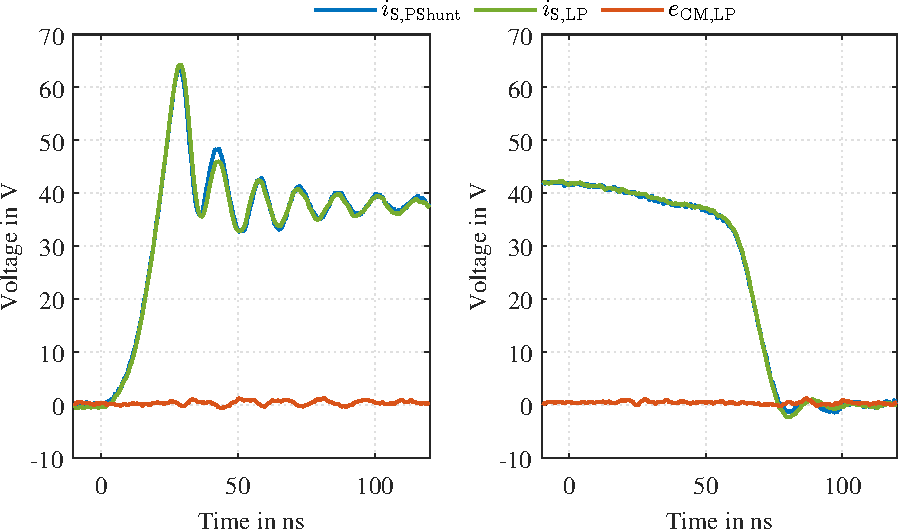
\includegraphics[scale=1]{figures/5_CurrentProbe/MS_Current_AvsPShunt_TD.pdf}
	\caption{Time-domain verification using a passive shunt.}\label{fig:MS_Current_AvsPShunt_TD}
\end{figure}

The measured waveforms show very good agreement between the active and passive shunts, both in the transient slope and in the observed overvoltage.
Only a small deviation appears in the second period of the main oscillation.
This deviation cannot be attributed to common-mode error, which is clearly much smaller.
It is therefore most likely caused by residual capacitive coupling from the voltage transient into the current shunt.


\subsection{Noise Behavior}
In a last step, the noise behavior of the active shunt is evaulated.
The measurement results are shown in \fref{fig:MS_Current_Noise}, where the noise floor of the active shunt is compared with the passive shunt.